% chapter3.tex — Design and Implementation
% This file is included via % chapter3.tex — Design and Implementation
% This file is included via % chapter3.tex — Design and Implementation
% This file is included via % chapter3.tex — Design and Implementation
% This file is included via \input{chapter3} in TFM_onamas.tex

This chapter presents the complete design and implementation of the demand forecasting system, following the CRISP-DM methodology introduced in Chapter~1. The work progresses from data acquisition and exploration through preprocessing, feature engineering, model development, evaluation, and finally the economic impact analysis that connects forecast accuracy to inventory cost savings.

\section{Data Origin}

\subsection{Data Acquisition}

The dataset used in this project was provided by the thesis supervisor and corresponds to real historical data from a company operating in the automotive sector. The data covers daily demand records for a portfolio of products, along with supplementary information on calendar events, promotional campaigns, and stock levels. All data was received in a single Microsoft Excel file (\texttt{Datos.xlsx}) containing four sheets, each representing a distinct dimension of the business context.

No personally identifiable information is present in the dataset, and all product references are anonymised using numerical identifiers, ensuring compliance with data privacy requirements as discussed in Section~\ref{s:etic}.

\subsection{Data Description}

The dataset comprises four tables, summarised in Table~\ref{tab:data_sheets}:

\begin{table}[H]
\centering
\small
\caption{Structure of the source dataset (\texttt{Datos.xlsx}).}
\label{tab:data_sheets}
\begin{tabular}{|l|l|r|p{5.5cm}|}
\hline
\textbf{Sheet} & \textbf{Key columns} & \textbf{Rows} & \textbf{Description} \\
\hline
Ventas (Sales) & producto, fecha, udsVenta & 654,588 & Daily unit sales per product \\
\hline
Calendario & fecha, bolOpen, bolHoliday & 732 & Calendar flags: business day and holiday indicators \\
\hline
Promociones & producto, fechaInicio, fechaFin & 1,894 & Promotional campaign periods per product \\
\hline
Stock & producto, fecha, udsStock & 654,588 & Daily stock levels per product \\
\hline
\end{tabular}
\end{table}

The sales sheet constitutes the core of the dataset, containing 654,588 daily observations across 894 unique products over a period of 732 days, spanning from November 2022 to November 2024. Each record represents the number of units sold for a specific product on a specific date.

The calendar sheet provides 732 daily records with two binary indicators: \texttt{bolOpen} (whether the business was open) and \texttt{bolHoliday} (whether the date was a public holiday). The promotions sheet contains 1,894 records defining promotional campaign windows through start and end dates for each product. The stock sheet mirrors the sales structure, recording the closing stock level for each product-date combination.

\subsection{Data Loading}

All four sheets were loaded into memory using the \texttt{pandas} library with the \texttt{openpyxl} engine. The sales and stock tables were merged on the shared keys \texttt{(producto, fecha)}, and the calendar information was joined on \texttt{fecha}. Promotional periods were transformed from date ranges into a binary indicator (\texttt{en\_promo}) at the product-date level, marking each observation as promotional or non-promotional based on whether the date fell within any active campaign for that product.

After merging, the resulting dataset contained 654,588 rows and served as the foundation for all subsequent analysis. The merged dataset was persisted in Apache Parquet format for efficient reloading in downstream scripts.


\section{Data Exploration}

\subsection{Data Summary}

An initial statistical summary of the target variable (\texttt{udsVenta}, units sold) revealed a highly skewed distribution. The mean daily sales per product were 1.42 units, with a median of zero and a standard deviation of 3.56. The maximum observed value was 99 units. This distribution reflects the nature of automotive parts demand, where the majority of product-day combinations register zero sales, punctuated by occasional larger orders.

Table~\ref{tab:sales_stats} presents the key descriptive statistics:

\begin{table}[H]
\centering
\small
\caption{Descriptive statistics of daily unit sales (\texttt{udsVenta}).}
\label{tab:sales_stats}
\begin{tabular}{|l|r|}
\hline
\textbf{Statistic} & \textbf{Value} \\
\hline
Count & 654,588 \\
Mean & 1.42 \\
Std. deviation & 3.56 \\
Median (50\%) & 0.00 \\
75th percentile & 1.00 \\
95th percentile & 7.00 \\
Maximum & 99 \\
Zero-sales proportion & 64.5\% \\
\hline
\end{tabular}
\end{table}

The high proportion of zero-sales observations (64.5\%) is a defining characteristic of this dataset and has important implications for model selection and evaluation, as discussed in subsequent sections.

\begin{figure}[H]
\centering
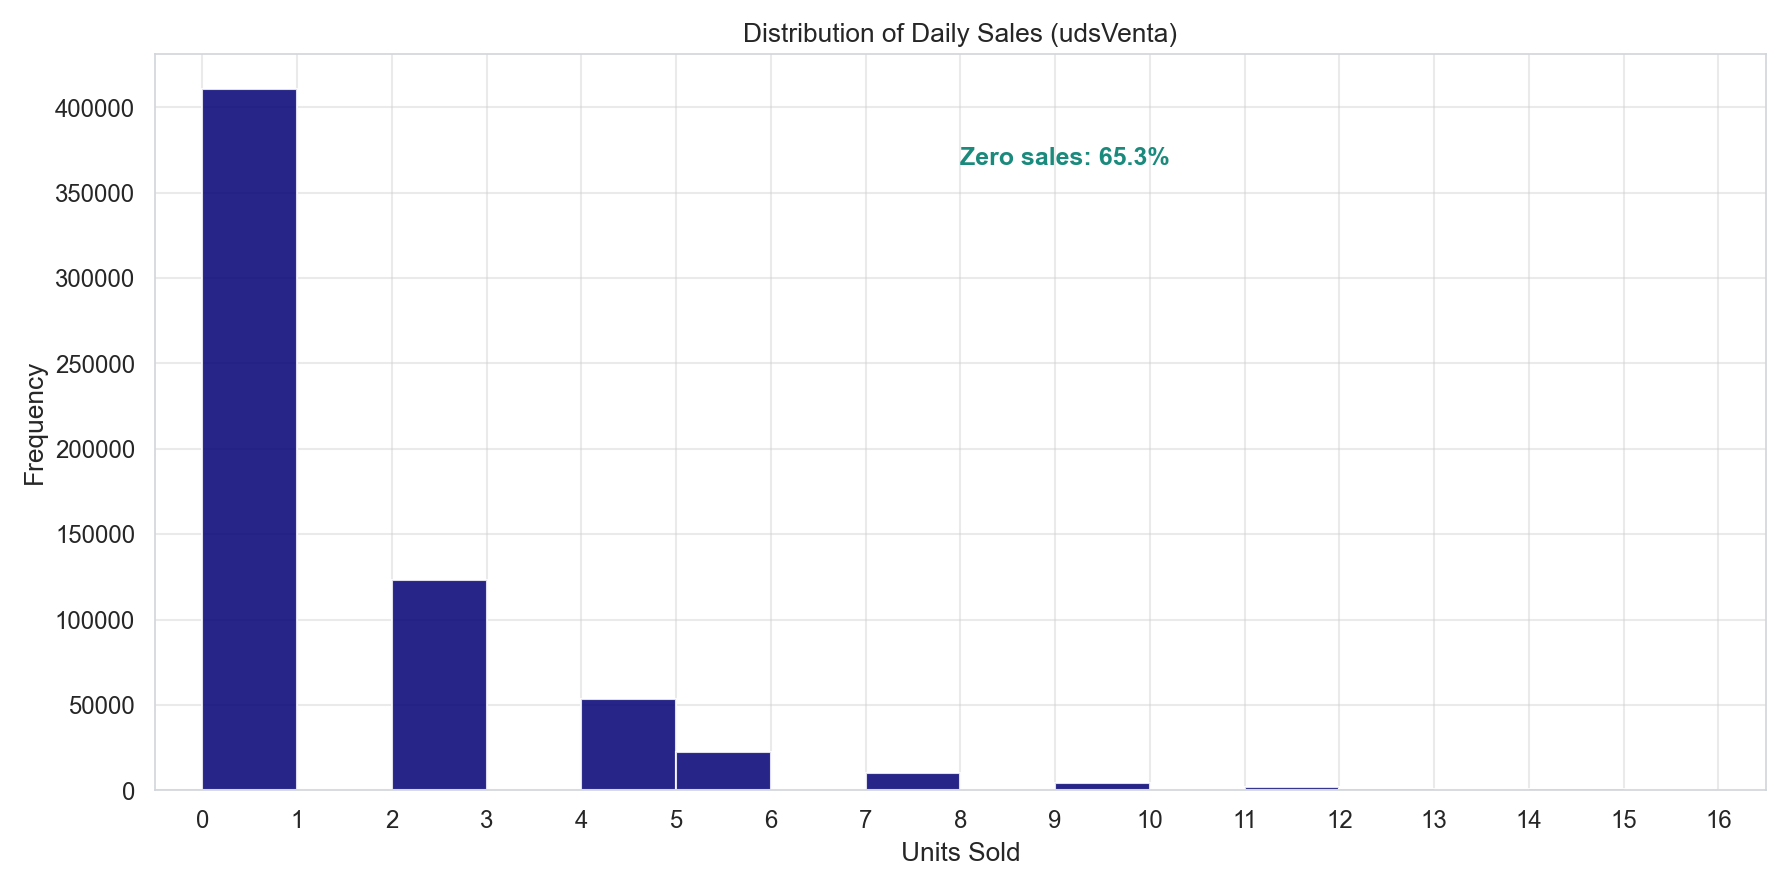
\includegraphics[width=0.85\textwidth]{figures/01_sales_distribution.png}
\caption{Distribution of daily unit sales (\texttt{udsVenta}). The histogram confirms the extreme right skew, with the majority of observations at zero.}
\label{fig:sales_distribution}
\end{figure}

\subsection{Statistical Analysis}

The exploratory analysis examined demand patterns across several dimensions:

\textbf{Day-of-week patterns.} Sales exhibit a clear weekly cycle, with the highest volumes on weekdays (Monday through Friday) and a sharp decline on Saturdays. Sunday sales are near zero, consistent with the business being closed on Sundays as indicated by the \texttt{bolOpen} calendar flag. This weekly seasonality motivates the inclusion of day-of-week features and the use of a lag-7 naive baseline (same weekday, previous week) as the primary benchmark.

\begin{figure}[H]
\centering
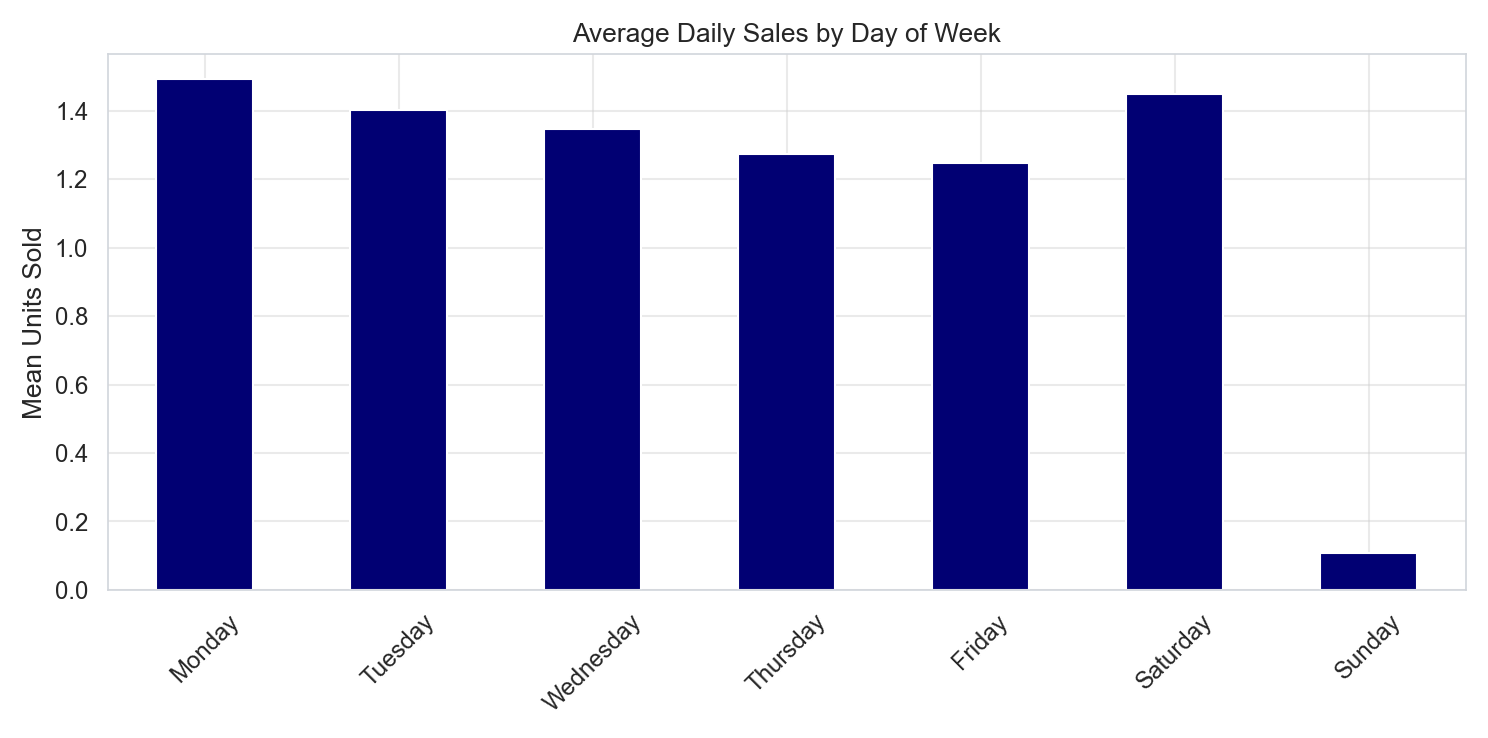
\includegraphics[width=0.85\textwidth]{figures/02_sales_by_day_of_week.png}
\caption{Average daily sales by day of the week. The weekly cycle is clearly visible, with near-zero sales on Sundays.}
\label{fig:sales_by_dow}
\end{figure}

\textbf{Monthly and seasonal patterns.} Monthly aggregated sales show moderate variation across the year, without a single dominant seasonal peak. However, certain months consistently show higher activity, suggesting that calendar-based features (month, week of year) may contribute predictive value.

\textbf{Promotional effects.} Comparing sales during promotional and non-promotional periods revealed that mean sales during promotions (1.83 units) were slightly higher than during non-promotional periods (1.38 units). However, the difference is modest, and the promotional flag alone does not capture the full complexity of promotional demand dynamics, which motivated the engineering of additional promotional features described in Section~3.4.

\begin{figure}[H]
\centering
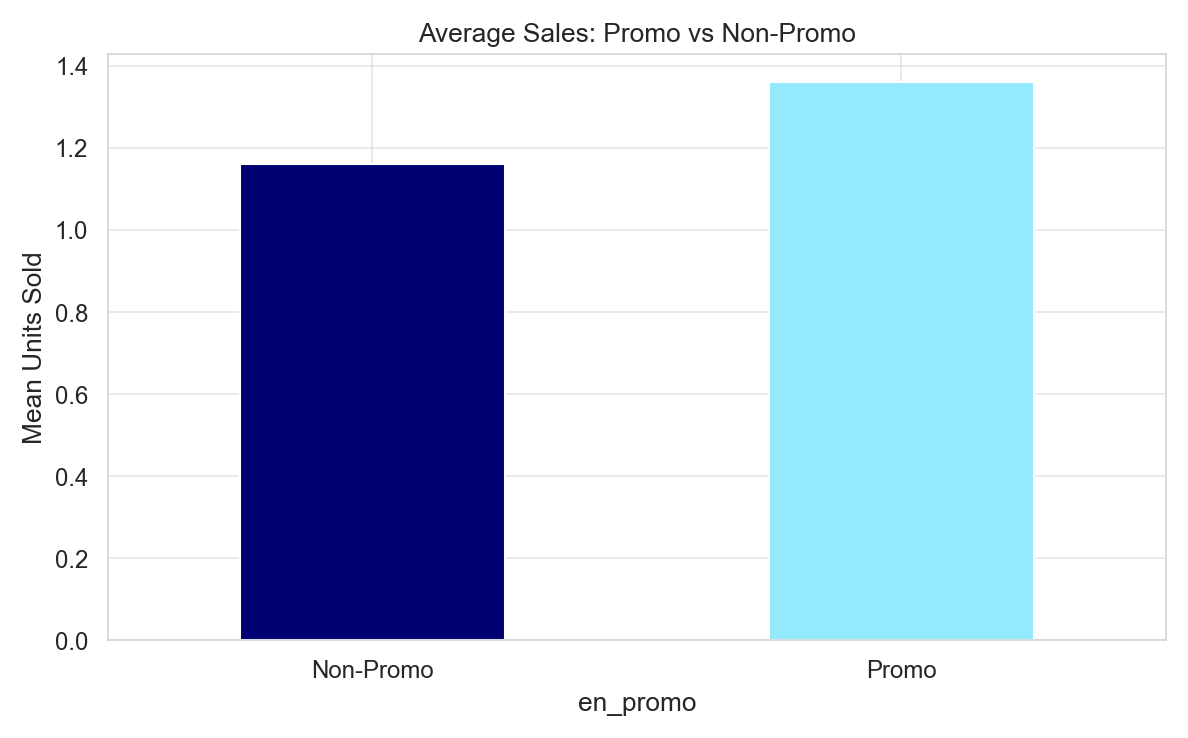
\includegraphics[width=0.85\textwidth]{figures/05_promo_vs_nonpromo.png}
\caption{Comparison of sales distributions during promotional and non-promotional periods.}
\label{fig:promo_vs_nonpromo}
\end{figure}

\textbf{Autocorrelation structure.} Autocorrelation analysis on a sample of products confirmed significant positive autocorrelation at lags 1, 7, 14, and 28, with the strongest signal at lag 7 (weekly periodicity). This finding directly supports the creation of lag features at these intervals and validates the choice of lag-7 as the naive baseline.

\begin{figure}[H]
\centering
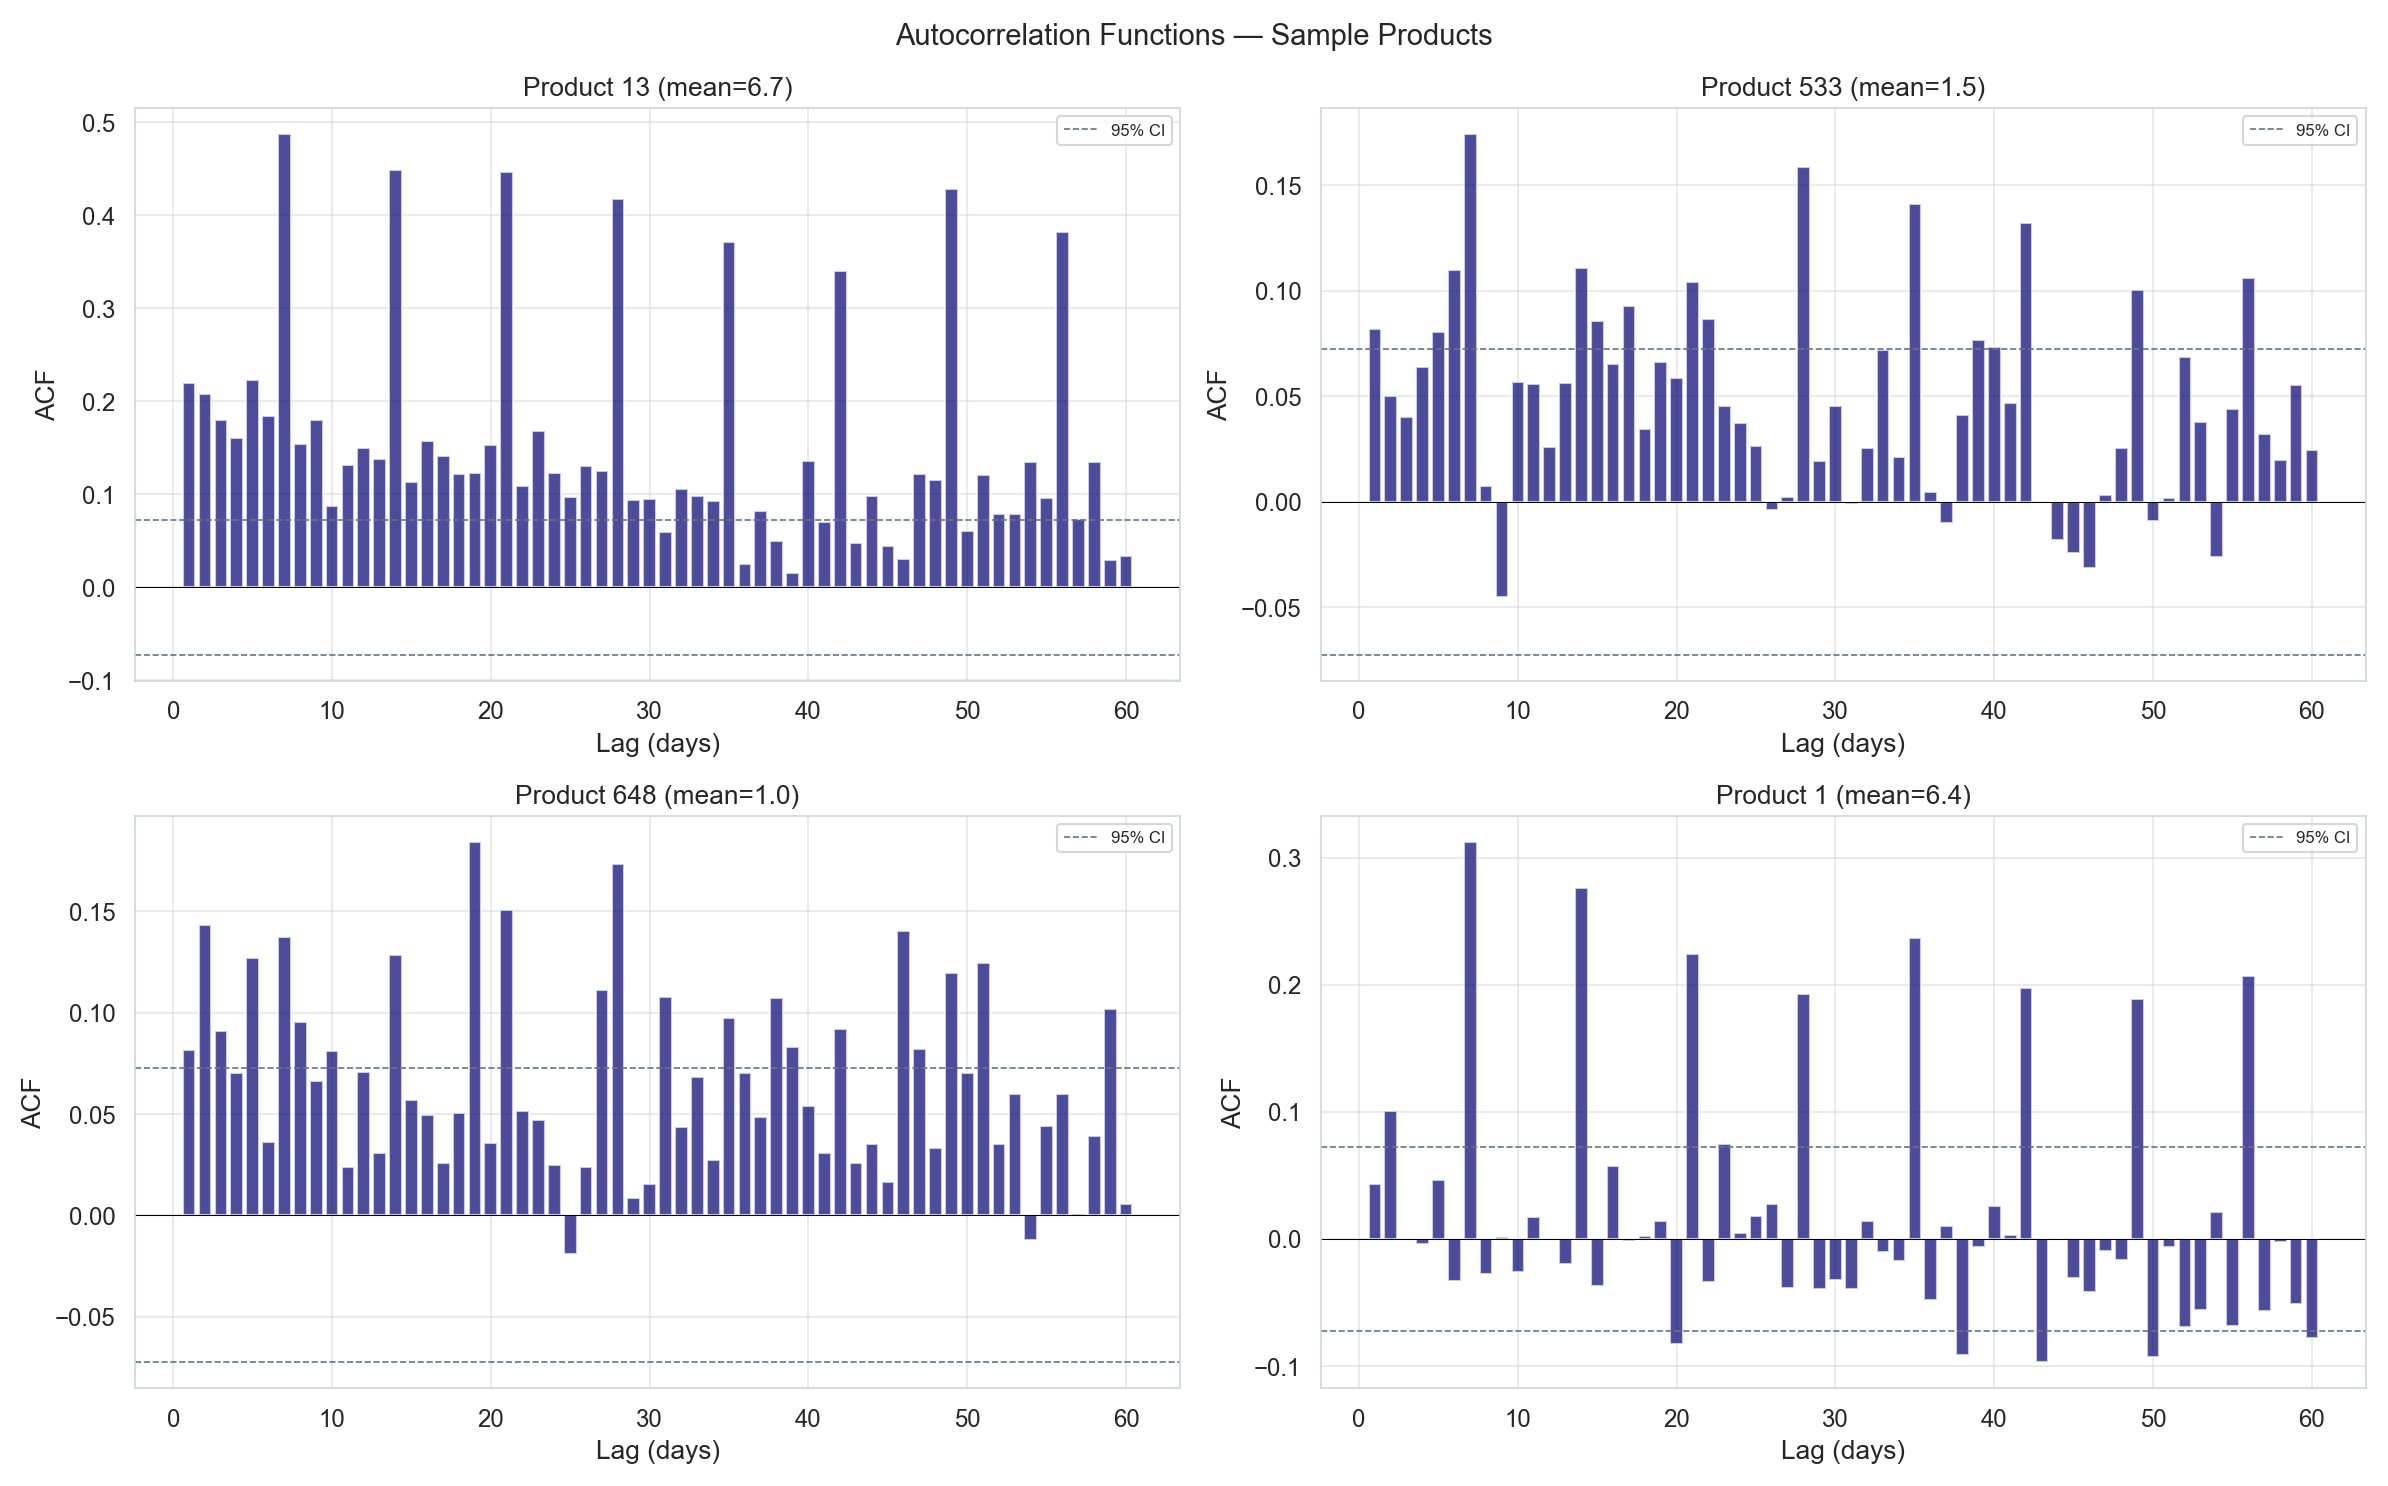
\includegraphics[width=0.85\textwidth]{figures/08_autocorrelation_sample.png}
\caption{Autocorrelation function (ACF) for a sample of products, showing significant positive autocorrelation at weekly intervals.}
\label{fig:autocorrelation}
\end{figure}

\subsection{Data Quality Analysis}

The data quality assessment identified the following issues:

\textbf{Missing values.} No explicit missing values were found in any of the four source tables. However, implicit gaps exist where lag features cannot be computed for the earliest dates in each product's history (addressed during feature engineering).

\textbf{Negative values.} No negative sales or stock values were present in this dataset.

\textbf{Stock breaks.} A stock break is defined as a day where both sales and stock are zero, potentially indicating that demand existed but could not be fulfilled due to inventory unavailability. Approximately 3.9\% of observations met this criterion. These were treated during data cleaning by imputing the product's historical mean sales for the corresponding weekday.

\textbf{Outliers.} Outlier detection was performed using a threshold of 1.75 times the interquartile range (IQR) per product. This identified approximately 11,400 observations (1.75\% of the dataset) as outliers, which were capped at the upper threshold value. The IQR-based approach was preferred over a fixed standard deviation threshold to account for the varying demand scales across products.


\section{Data Preparation}

\subsection{Data Cleaning}

The data cleaning process addressed the two quality issues identified during exploration:

\begin{enumerate}
    \item \textbf{Stock break imputation:} For observations where both \texttt{udsVenta} and \texttt{udsStock} were zero, the sales value was replaced with the mean sales for that product on the same weekday, computed over the preceding 30 days. This approach assumes that zero sales on a day with zero stock reflects a supply-side constraint rather than genuine zero demand, and uses a localised historical average to provide a reasonable demand estimate.

    \item \textbf{Outlier capping:} Values exceeding 1.75 $\times$ IQR above the 75th percentile for each product were capped at the threshold value. This preserves the general distribution shape while limiting the influence of extreme observations on model training. A total of 11,400 values (1.75\% of the dataset) were capped.
\end{enumerate}

After cleaning, the dataset retained its original 654,588 rows with no records removed, ensuring that the temporal continuity required for lag feature computation was preserved.

\subsection{Data Transformation}

The date column (\texttt{fecha}) was parsed into a \texttt{datetime} type, and the dataset was sorted by product and date to ensure correct temporal ordering for all subsequent operations. The promotional periods from the source data were transformed from date-range format into a daily binary indicator (\texttt{en\_promo}), assigned at the product-date level.

No logarithmic or power transformations were applied to the target variable. While such transformations can stabilise variance in skewed distributions, the tree-based models used in this work (Random Forest, XGBoost, LightGBM) are inherently robust to non-normal distributions and do not require target transformation for effective learning.

\subsection{Data Scaling}

Feature scaling (standardisation or normalisation) was not applied for the tree-based models, as decision tree ensembles are invariant to monotonic transformations of input features. The split-based learning mechanism of these algorithms operates on feature rankings rather than absolute values, making scaling unnecessary.

For the LSTM model, min-max normalisation was applied to all input features to facilitate gradient-based optimisation. Each feature was scaled to the $[0, 1]$ range using the training set statistics, and the same transformation was applied to the validation and test sets to prevent information leakage. Predictions were inverse-transformed back to the original scale before computing evaluation metrics.

\section{Feature Engineering}

Feature engineering is a central component of this work. A comprehensive set of 36 engineered features was designed to capture temporal dependencies, demand dynamics, and promotional effects. The features are organised into five categories, summarised in Table~\ref{tab:features}.

\begin{table}[H]
\centering
\small
\caption{Engineered features by category.}
\label{tab:features}
\begin{tabular}{|l|p{7cm}|r|}
\hline
\textbf{Category} & \textbf{Features} & \textbf{Count} \\
\hline
Original variables & udsStock, bolOpen, bolHoliday, en\_promo & 4 \\
\hline
Calendar features & year, month, day\_of\_week, week\_of\_year, week\_of\_month, is\_weekend, is\_month\_start, is\_month\_end & 8 \\
\hline
Lag features & lag\_1, lag\_7, lag\_14, lag\_28 & 4 \\
\hline
Rolling statistics & roll\_mean/std/min/max at 7, 14, and 28-day windows; ewma\_7, ewma\_28 & 14 \\
\hline
Promotional features & days\_since\_promo\_end, post\_promo\_7d, promo\_x\_lag7 & 3 \\
\hline
Product-level statistics & prod\_mean\_sales, prod\_std\_sales, prod\_median\_sales & 3 \\
\hline
\multicolumn{2}{|r|}{\textbf{Total}} & \textbf{36} \\
\hline
\end{tabular}
\end{table}

\textbf{Lag features} capture the autoregressive structure identified during exploration. The lag-7 feature (same weekday, previous week) serves dual purpose: it is used directly as the naive baseline forecast and as an input feature for the machine learning models. Lags at 1, 14, and 28 days capture short-term momentum, biweekly patterns, and monthly cycles respectively.

\textbf{Rolling statistics} provide smoothed representations of recent demand behaviour. For each window size (7, 14, and 28 days), the mean, standard deviation, minimum, and maximum of past sales are computed. Additionally, exponentially weighted moving averages (EWMA) with spans of 7 and 28 days provide adaptive smoothing that gives greater weight to more recent observations.

\textbf{Promotional features} go beyond the binary indicator to capture the temporal dynamics of promotions. The \texttt{days\_since\_promo\_end} feature tracks the recency of the last promotional period, \texttt{post\_promo\_7d} flags the week immediately following a promotion (to capture post-promotional demand depression), and \texttt{promo\_x\_lag7} is an interaction term between the promotional flag and the lag-7 sales value.

All lag and rolling features were computed strictly using past data to prevent information leakage. Observations where lag features could not be computed (the first 28 days of each product's history) were dropped, reducing the dataset from 654,588 to 629,370 rows. The final feature matrix was saved in Parquet format for use in the modelling phase.

\begin{figure}[H]
\centering
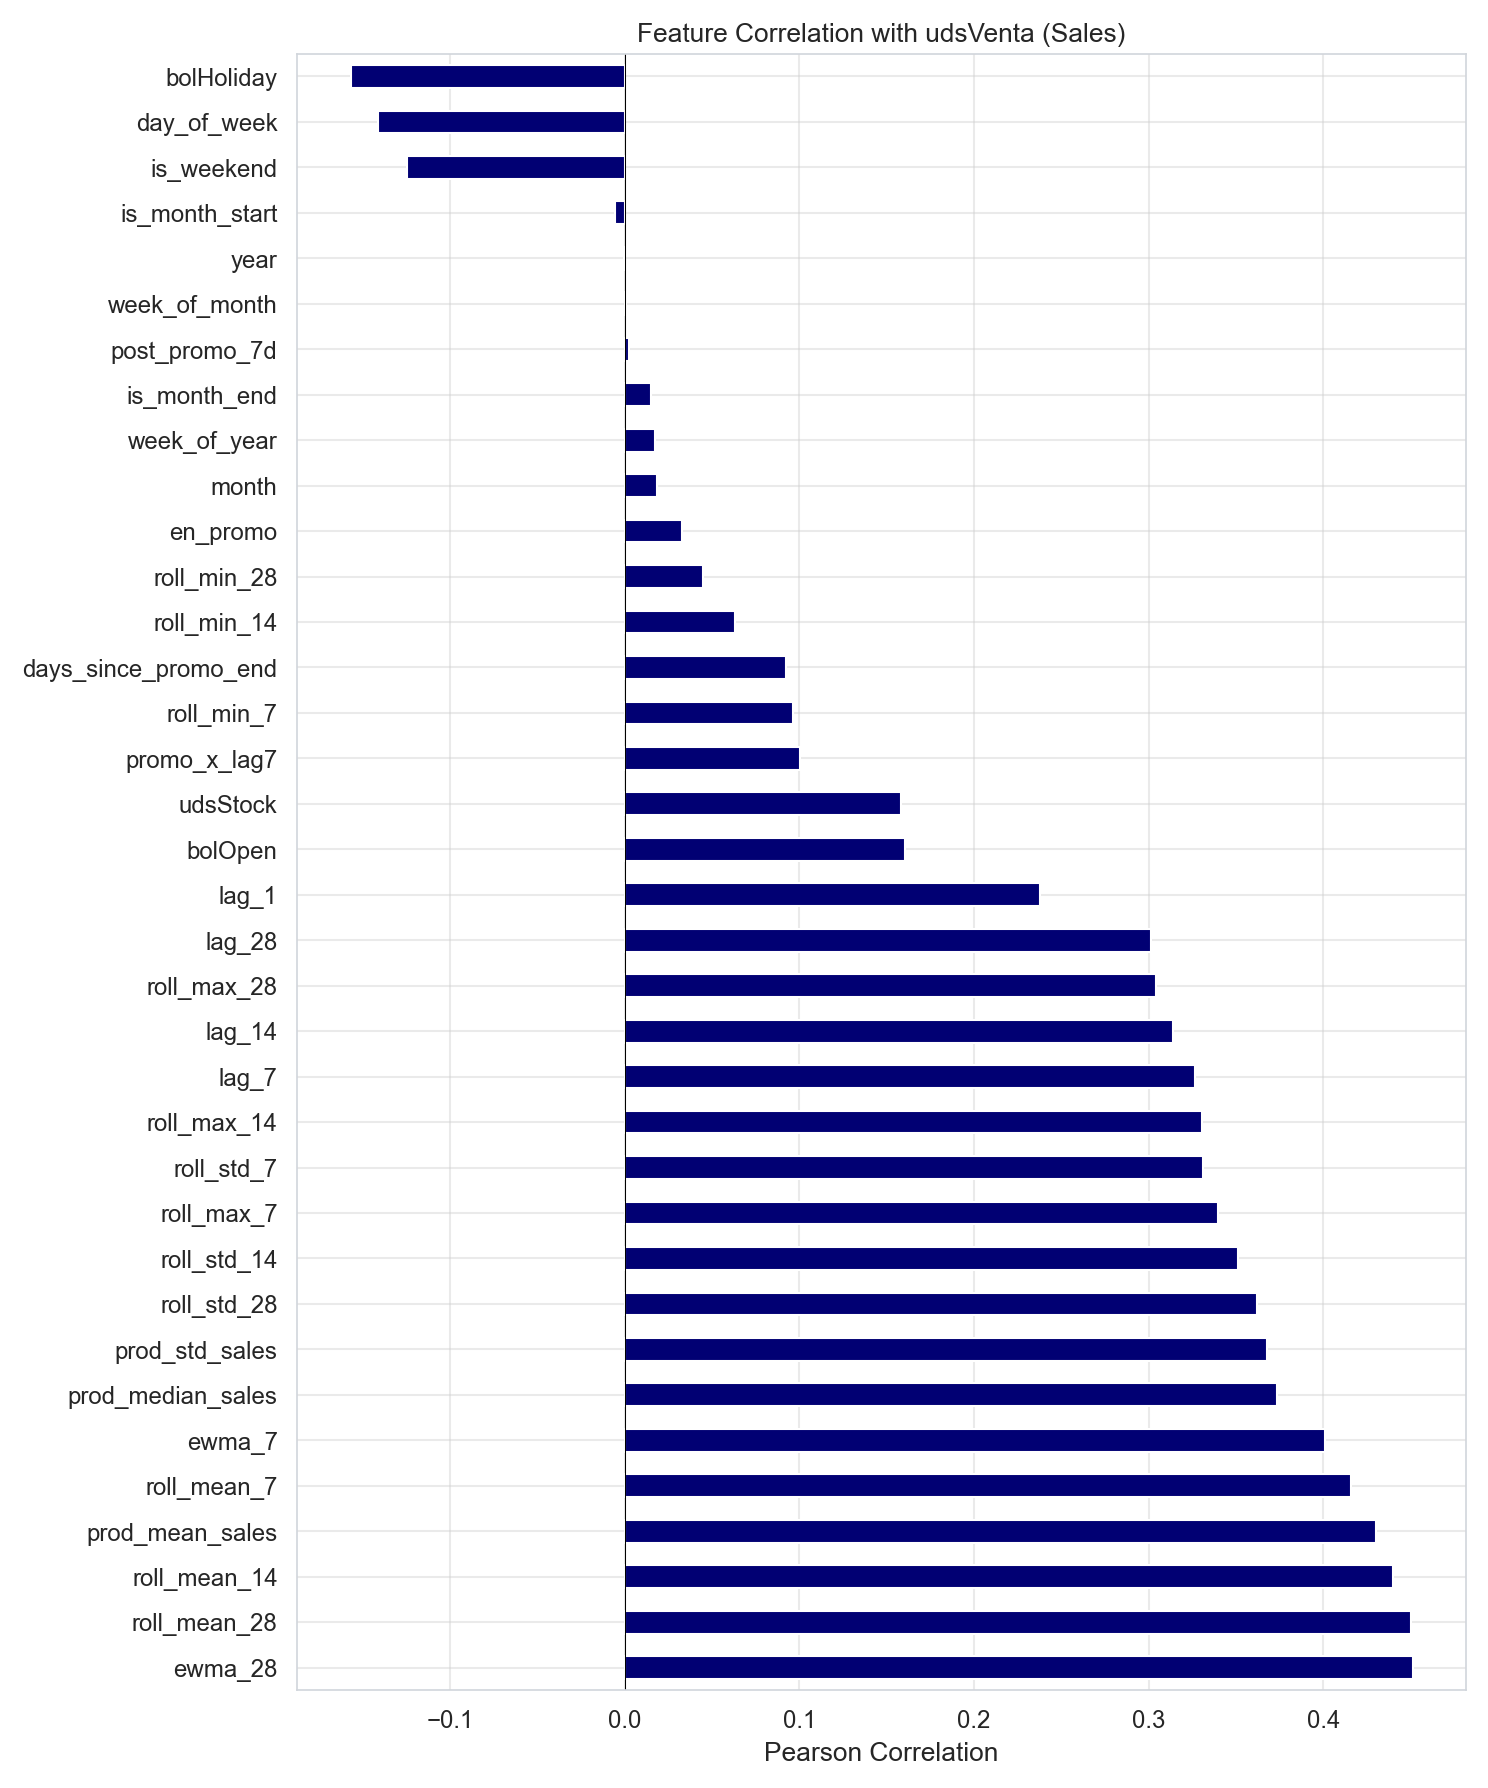
\includegraphics[width=0.95\textwidth]{figures/10_feature_correlations.png}
\caption{Correlation matrix of the engineered features. Strong correlations are visible among rolling statistics at different window sizes, confirming the presence of redundant but complementary temporal signals.}
\label{fig:feature_correlations}
\end{figure}


\section{Modelling}

\subsection{Model Selection}

Four forecasting approaches were implemented, spanning a naive baseline and three gradient boosting / ensemble methods:

\begin{enumerate}
    \item \textbf{Naive baseline (lag-7):} The simplest possible forecast, predicting that demand on any given day equals the demand observed on the same weekday of the previous week. This baseline exploits the strong weekly autocorrelation identified during exploration and provides a meaningful benchmark against which machine learning models must demonstrate improvement.

    \item \textbf{ARIMA (Seasonal):} A classical time series approach fitted per product using the \texttt{auto\_arima} implementation from the \texttt{pmdarima} library. Each product's demand series was modelled with seasonal ARIMA (SARIMA) with weekly periodicity ($m=7$), automatically selecting the optimal $(p,d,q)(P,D,Q)_7$ orders via stepwise search. ARIMA serves as the classical statistical baseline, representing the best that traditional time series methods can achieve without engineered features.

    \item \textbf{Random Forest:} An ensemble of decision trees trained on bootstrap samples with random feature subsets \citep{hyndman2021forecasting}. Random Forest provides robust predictions with built-in protection against overfitting through bagging and feature randomisation.

    \item \textbf{XGBoost:} A gradient boosting framework that builds trees sequentially, with each tree correcting the errors of its predecessors. XGBoost incorporates L1 and L2 regularisation, column subsampling, and efficient handling of sparse data, making it well-suited to the high proportion of zero-demand observations in this dataset.

    \item \textbf{LightGBM:} A gradient boosting implementation that uses histogram-based splitting and leaf-wise tree growth, offering faster training times than XGBoost while maintaining competitive accuracy. LightGBM was among the dominant algorithms in the M5 forecasting competition \citep{makridakis2021m5findings}.

    \item \textbf{LSTM (Long Short-Term Memory):} A recurrent neural network architecture designed to capture long-range temporal dependencies in sequential data \citep{hochreiter1997lstm}. Unlike tree-based methods, which rely on engineered lag features, LSTM processes input data as ordered sequences, with its internal gating mechanism allowing it to selectively retain or discard information from previous time steps. The model was implemented in PyTorch with a single LSTM layer (32 hidden units), trained on standardised features using 14-day input sequences.
\end{enumerate}

All tree-based models were trained on the full set of 33 input features (the 36 engineered features minus the 3 product-level statistics used only for reference). ARIMA was fitted per product on the raw sales series without engineered features, as is standard for classical time series methods. The LSTM model received the same 33 features as the tree models, but processed them as ordered sequences rather than independent observations. All predictions were clipped to a minimum of zero to prevent negative forecast values.

\subsection{Definition of Accuracy Indicators}

Four complementary metrics were used to evaluate forecast performance, as introduced in Chapter~2:

\begin{itemize}
    \item \textbf{MAE} (Mean Absolute Error): average absolute deviation between forecast and actual demand, in the same units as the target variable.
    \item \textbf{RMSE} (Root Mean Squared Error): penalises larger errors more heavily than MAE, providing a measure sensitive to occasional large deviations.
    \item \textbf{MAPE} (Mean Absolute Percentage Error): expresses errors as a percentage of actual demand, computed only for observations where actual demand is greater than zero to avoid division by zero.
    \item \textbf{$\sigma_e$} (forecast error standard deviation): the standard deviation of the residuals ($D_t - F_t$), which directly enters the safety stock calculation (Equation~\ref{eq:safety_stock}) and thus provides the link between forecast accuracy and inventory cost.
\end{itemize}

\subsection{Definition of Training and Validation Periods}

A rolling forecast origin validation strategy was adopted to provide a realistic assessment of out-of-sample performance by simulating the sequential nature of real forecasting decisions \citep{makridakis2021m5findings}.

Three validation folds were defined, each with a 30-day test window, working backwards from the most recent date in the dataset:

\begin{table}[H]
\centering
\small
\caption{Rolling forecast origin validation folds.}
\label{tab:folds}
\begin{tabular}{|c|c|c|c|}
\hline
\textbf{Fold} & \textbf{Training period end} & \textbf{Test period} & \textbf{Test days} \\
\hline
1 & 2024-09-06 & 2024-09-07 -- 2024-10-06 & 30 \\
2 & 2024-10-06 & 2024-10-07 -- 2024-11-05 & 30 \\
3 & 2024-10-06 & 2024-10-07 -- 2024-11-05 & 30 \\
\hline
\end{tabular}
\end{table}

For each fold, the training set includes all data up to the fold's cutoff date (expanding window), and the model is evaluated on the subsequent 30-day period. Final reported metrics are averaged across all three folds.

\subsection{Hyperparameter Tuning}

Hyperparameters for all three machine learning models were optimised using Optuna \citep{makridakis2021m5findings}, a Bayesian optimisation framework that efficiently explores the parameter space using a Tree-structured Parzen Estimator (TPE) sampler.

To balance computational cost with tuning quality, the optimisation was conducted on a representative subset of 50 randomly sampled products using the first validation fold. Each model was allocated 30 Optuna trials, with RMSE on the validation set as the objective function. The optimised hyperparameters were then applied to the full dataset across all validation folds.

Table~\ref{tab:tuned_params} presents the key tuned hyperparameters for each model:

\begin{table}[H]
\centering
\small
\caption{Optimised hyperparameters via Optuna (30 trials per model).}
\label{tab:tuned_params}
\begin{tabular}{|l|l|r|}
\hline
\textbf{Model} & \textbf{Parameter} & \textbf{Value} \\
\hline
\multirow{5}{*}{LightGBM} & n\_estimators & 300 \\
 & learning\_rate & 0.011 \\
 & num\_leaves & 75 \\
 & max\_depth & 4 \\
 & min\_child\_samples & 25 \\
\hline
\multirow{5}{*}{XGBoost} & n\_estimators & 350 \\
 & learning\_rate & 0.019 \\
 & max\_depth & 3 \\
 & min\_child\_weight & 10 \\
 & subsample & 0.90 \\
\hline
\multirow{4}{*}{Random Forest} & n\_estimators & 100 \\
 & max\_depth & 5 \\
 & min\_samples\_leaf & 16 \\
 & max\_features & 0.30 \\
\hline
\end{tabular}
\end{table}

The relatively shallow tree depths (3--5) and conservative learning rates (0.011--0.019) selected by the optimiser suggest that the models benefit from regularisation, which is consistent with the high proportion of zero-demand observations in the dataset.


\section{Evaluation}

\subsection{Accuracy Results Obtained}

Table~\ref{tab:results_summary} presents the average performance of each model across the three validation folds:

\begin{table}[H]
\centering
\small
\caption{Average forecast accuracy across three rolling validation folds.}
\label{tab:results_summary}
\begin{tabular}{|l|r|r|r|r|}
\hline
\textbf{Model} & \textbf{MAE} & \textbf{RMSE} & \textbf{MAPE (\%)} & \textbf{$\sigma_e$} \\
\hline
XGBoost & 1.366 & 2.155 & 52.2 & 2.154 \\
LightGBM & 1.373 & 2.158 & 51.7 & 2.158 \\
Random Forest & 1.394 & 2.176 & 51.6 & 2.176 \\
ARIMA$^\dagger$ & 1.443 & 2.220 & 59.8 & 2.219 \\
LSTM & 1.522 & 2.235 & 49.8 & 2.223 \\
Naive (lag-7) & 1.661 & 3.091 & 86.0 & 3.091 \\
\hline
\end{tabular}
\begin{flushleft}
\footnotesize{$^\dagger$ ARIMA evaluated on 50 sampled products due to per-product fitting cost.}
\end{flushleft}
\end{table}

All three tree-based machine learning models substantially outperform both the naive baseline and the classical/deep learning alternatives. XGBoost achieves the lowest RMSE (2.155), followed closely by LightGBM (2.158) and Random Forest (2.176). The RMSE improvement over the naive baseline ranges from 27.9\% (LSTM) to 30.3\% (XGBoost).

\begin{figure}[H]
\centering
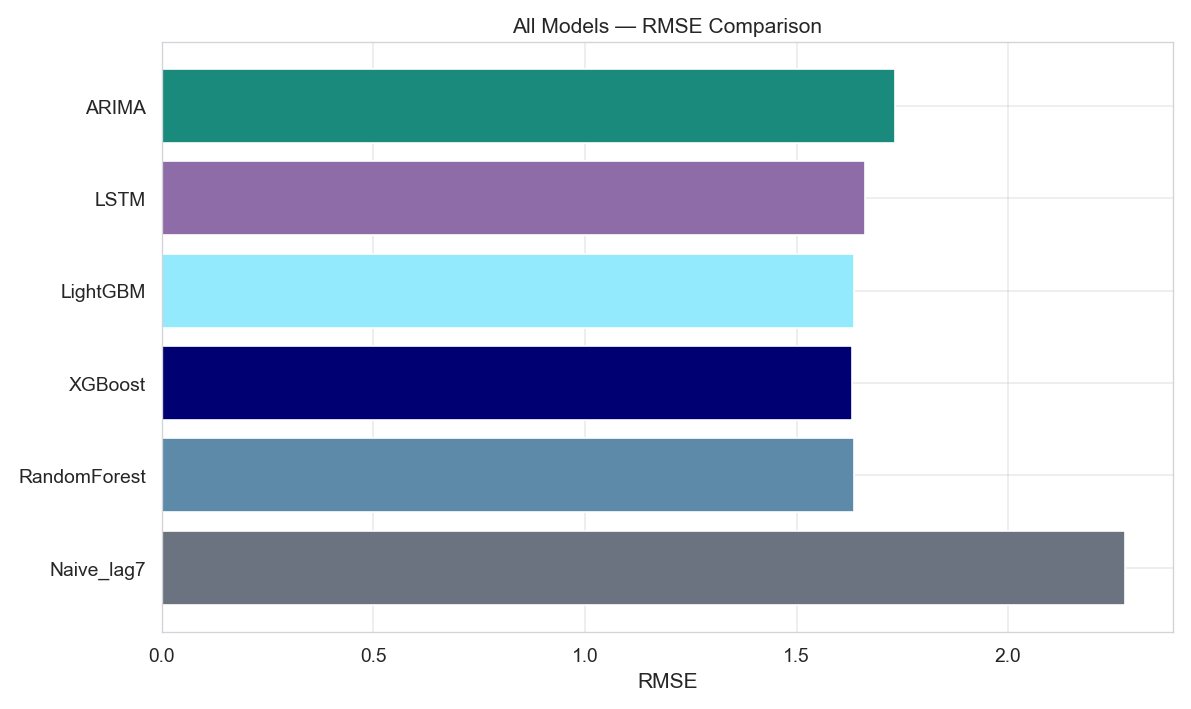
\includegraphics[width=0.85\textwidth]{figures/24_all_models_comparison.png}
\caption{Comparison of forecast accuracy (RMSE) across all six models. The three tree-based models form a tight cluster, substantially outperforming both classical and deep learning alternatives.}
\label{fig:all_models_comparison}
\end{figure}

ARIMA and LSTM occupy an intermediate position: both significantly outperform the naive baseline (RMSE reductions of 28.2\% and 27.7\% respectively) but fall short of the tree-based models. This result is consistent with the findings of the M5 forecasting competition \citep{makridakis2021m5findings}, where gradient boosting algorithms consistently outperformed both classical statistical methods and standalone deep learning approaches. The LSTM's slightly lower MAPE (49.8\%) but higher RMSE suggests it handles the zero-heavy distribution differently from tree models, producing fewer large percentage errors but occasionally larger absolute deviations.

\subsection{Comparison of Results Across Models}

\textbf{Promotional vs. non-promotional performance.} Table~\ref{tab:promo_results} compares model performance across demand segments:

\begin{table}[H]
\centering
\small
\caption{Model performance by demand segment (last validation fold).}
\label{tab:promo_results}
\begin{tabular}{|l|l|r|r|r|r|}
\hline
\textbf{Segment} & \textbf{Model} & \textbf{MAE} & \textbf{RMSE} & \textbf{MAPE (\%)} & \textbf{$\sigma_e$} \\
\hline
\multirow{4}{*}{Non-Promo} & XGBoost & 1.299 & 2.055 & 52.3 & 2.055 \\
 & LightGBM & 1.308 & 2.058 & 51.8 & 2.058 \\
 & Random Forest & 1.327 & 2.073 & 51.6 & 2.073 \\
 & Naive (lag-7) & 1.565 & 2.969 & 85.9 & 2.969 \\
\hline
\multirow{4}{*}{Promo} & XGBoost & 1.917 & 2.844 & 51.7 & 2.836 \\
 & LightGBM & 1.911 & 2.851 & 51.4 & 2.838 \\
 & Random Forest & 1.944 & 2.884 & 51.6 & 2.873 \\
 & Naive (lag-7) & 2.448 & 3.956 & 86.9 & 3.955 \\
\hline
\end{tabular}
\end{table}

Promotional demand is consistently harder to predict across all models, with RMSE values approximately 38\% higher than for non-promotional periods. However, the ML models maintain their advantage over the naive baseline in both segments, with RMSE improvements of approximately 28\% for non-promotional and 28\% for promotional demand.

\textbf{Per-product RMSE distribution.} Analysis at the individual product level reveals that LightGBM achieves a median per-product RMSE of 1.65, compared to 2.36 for the naive baseline. The improvement is not uniform: some products see RMSE reductions exceeding 15 units, while approximately 10 products show marginally worse performance with ML than with the naive approach. These products tend to have very low and stable demand where the simple lag-7 heuristic is already near-optimal.

\begin{figure}[H]
\centering
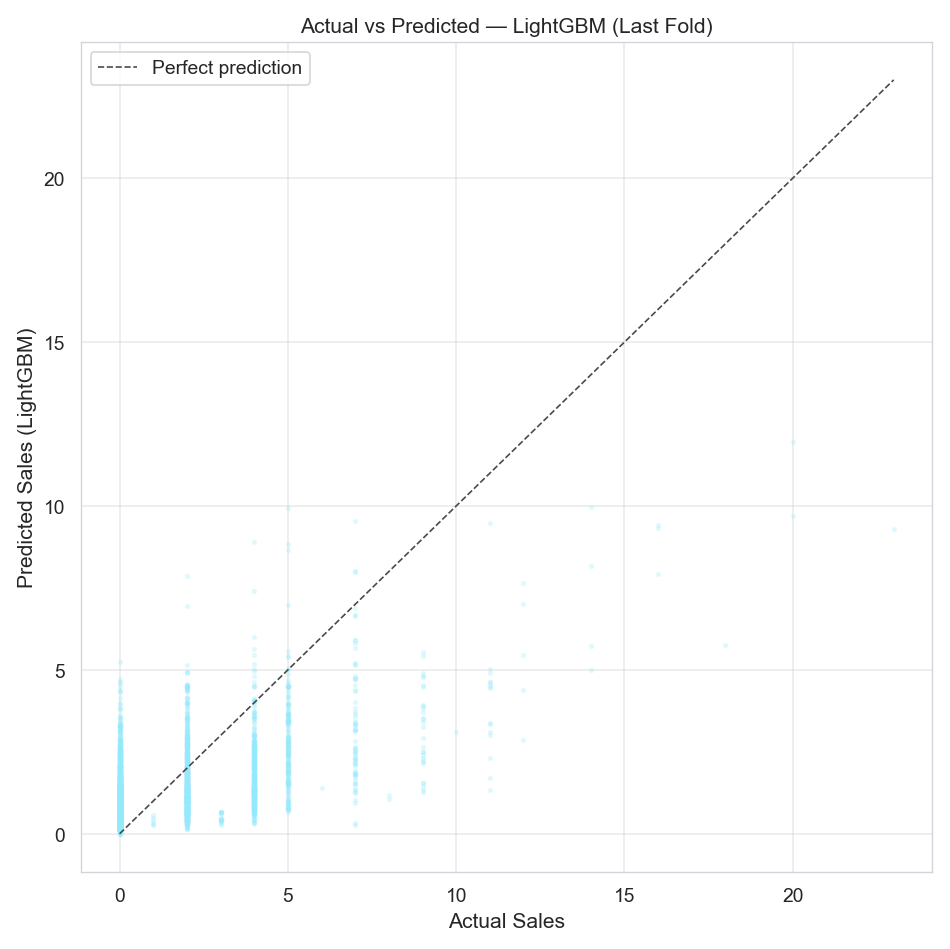
\includegraphics[width=0.85\textwidth]{figures/13_actual_vs_predicted_lgbm.png}
\caption{Actual vs.\ predicted sales for LightGBM on a sample of products. Points near the diagonal indicate accurate predictions; the cluster near the origin reflects the high proportion of zero-demand observations.}
\label{fig:actual_vs_predicted}
\end{figure}

\begin{figure}[H]
\centering
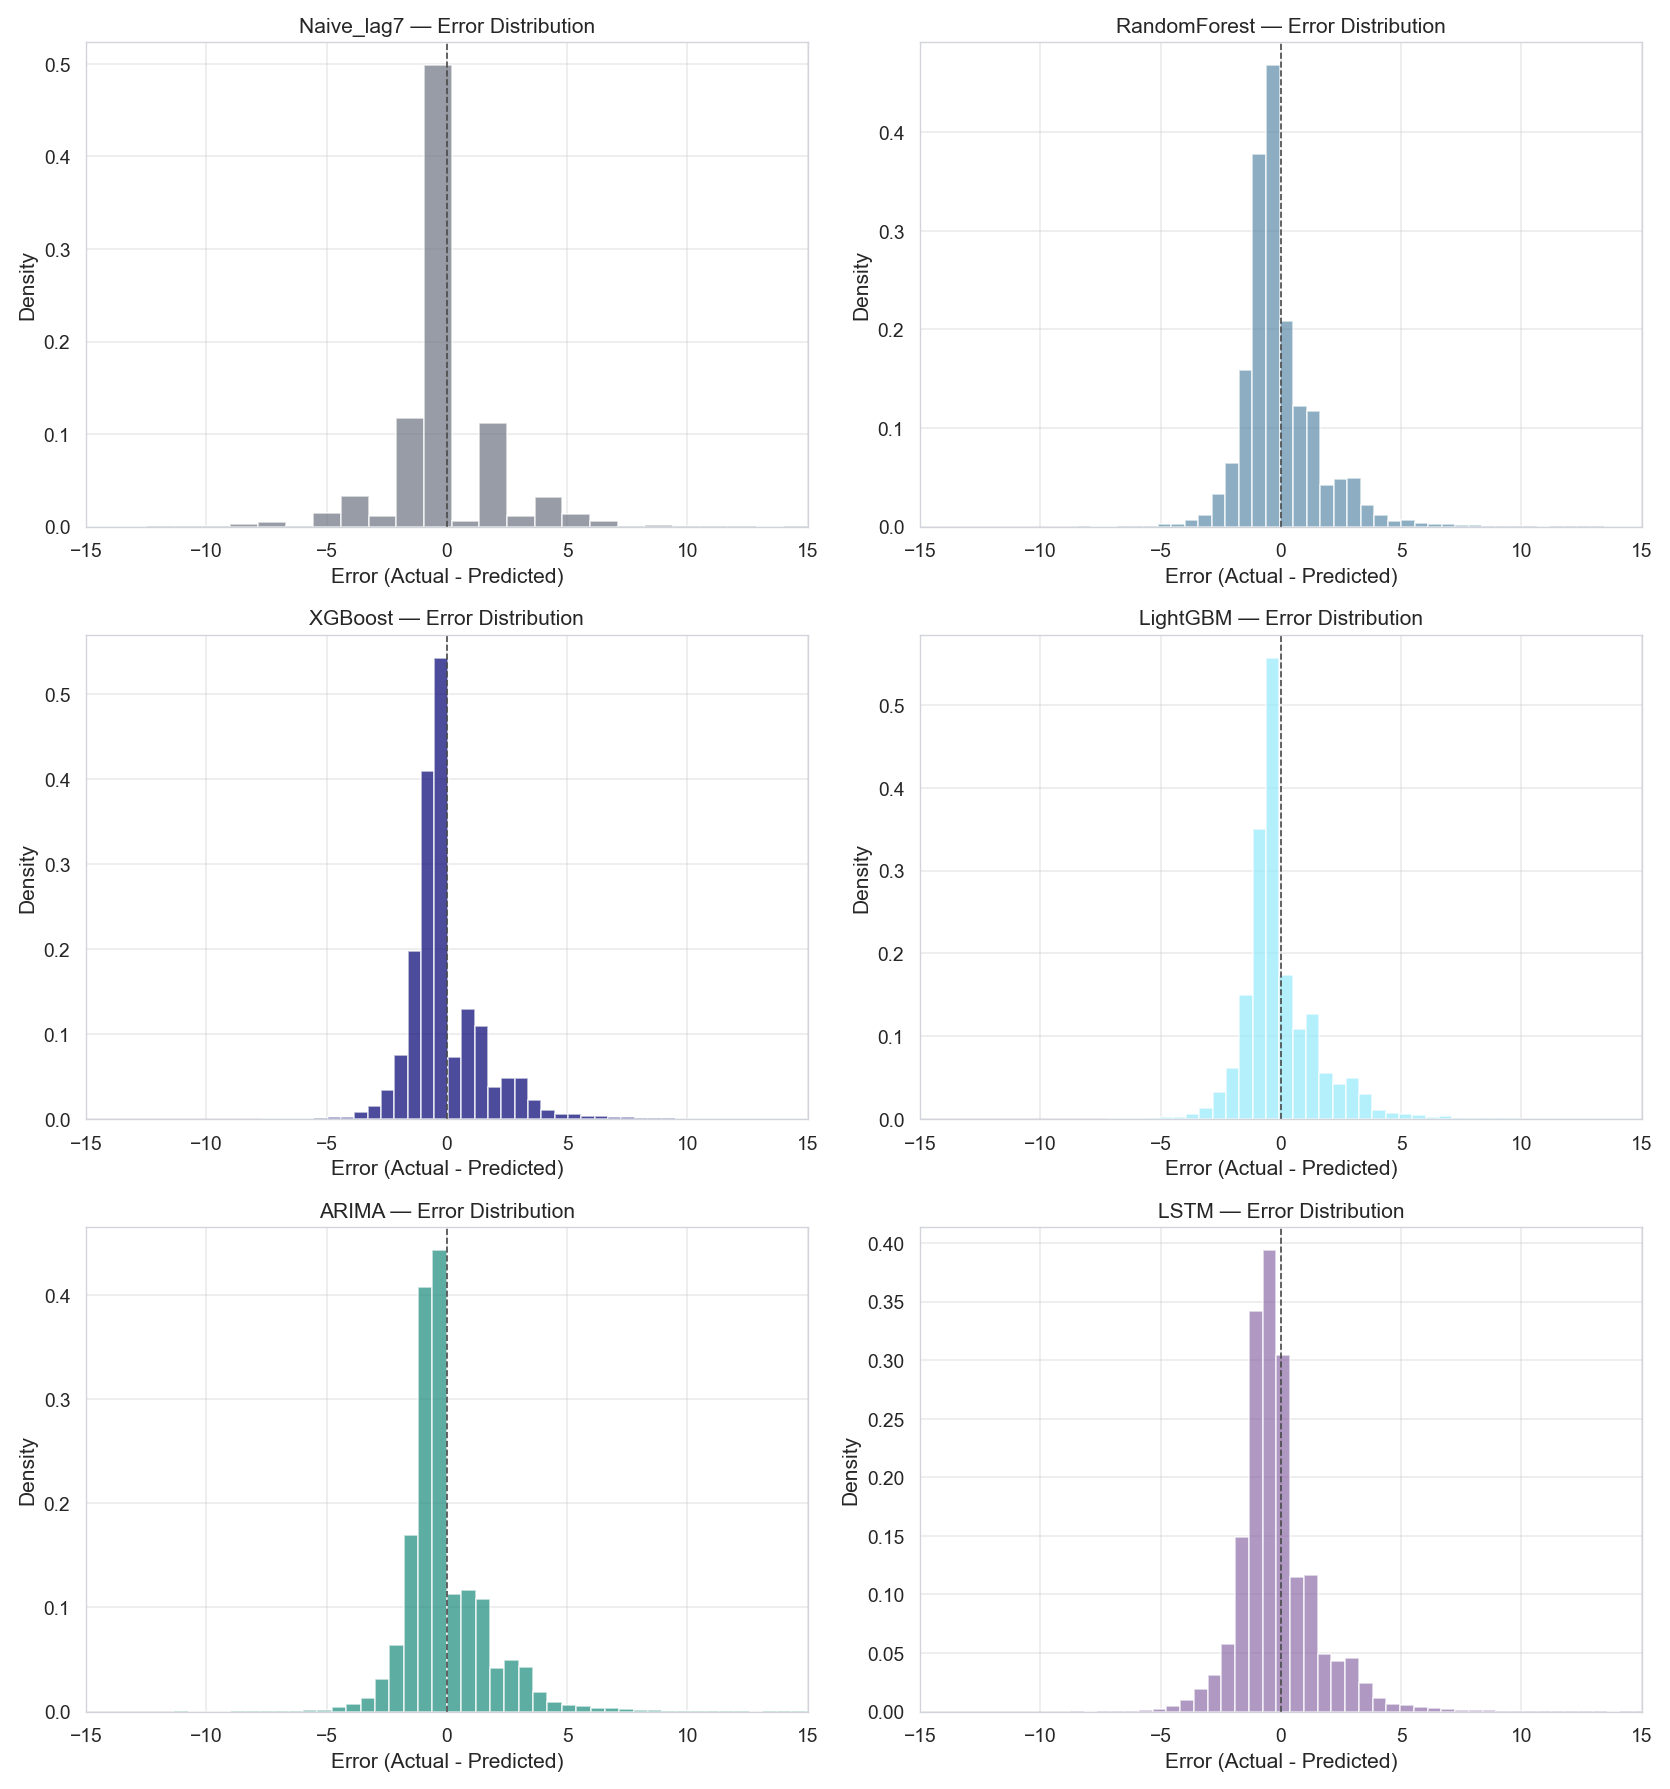
\includegraphics[width=0.85\textwidth]{figures/17_error_distributions.png}
\caption{Distribution of forecast errors by model. The ML models produce tighter, more symmetric error distributions compared to the naive baseline.}
\label{fig:error_distributions}
\end{figure}

\begin{figure}[H]
\centering
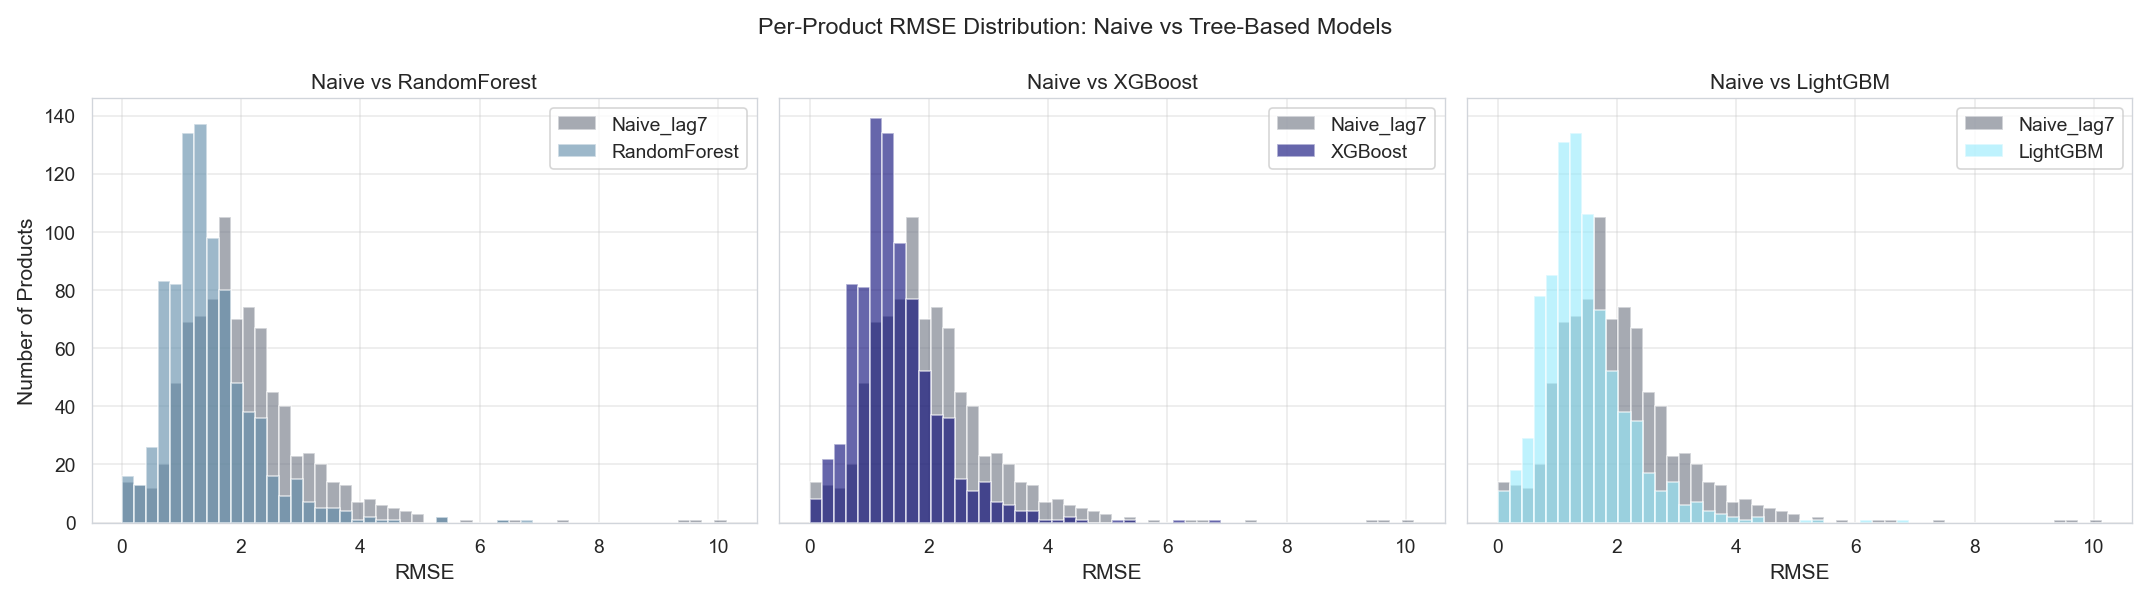
\includegraphics[width=0.85\textwidth]{figures/18_per_product_rmse_dist.png}
\caption{Distribution of per-product RMSE values. The ML models shift the distribution towards lower RMSE values compared to the naive baseline.}
\label{fig:per_product_rmse}
\end{figure}

\textbf{SHAP feature importance.} To understand the drivers of model predictions, SHAP (SHapley Additive exPlanations) analysis was performed on the LightGBM model. Table~\ref{tab:shap_top10} presents the ten most influential features:

\begin{table}[H]
\centering
\small
\caption{Top 10 features by mean absolute SHAP value (LightGBM).}
\label{tab:shap_top10}
\begin{tabular}{|r|l|r|}
\hline
\textbf{Rank} & \textbf{Feature} & \textbf{Mean $|$SHAP$|$} \\
\hline
1 & ewma\_28 & 0.524 \\
2 & bolHoliday & 0.295 \\
3 & roll\_mean\_28 & 0.150 \\
4 & day\_of\_week & 0.079 \\
5 & udsStock & 0.063 \\
6 & roll\_max\_28 & 0.046 \\
7 & lag\_28 & 0.025 \\
8 & bolOpen & 0.022 \\
9 & roll\_mean\_14 & 0.017 \\
10 & roll\_max\_14 & 0.016 \\
\hline
\end{tabular}
\end{table}

The 28-day EWMA emerges as the single most important predictor, followed by the holiday indicator and the 28-day rolling mean. This confirms that the model relies heavily on smoothed representations of recent demand history, with calendar effects providing secondary but significant predictive power. Notably, the longer-horizon features (28-day windows) dominate over shorter-horizon ones (7-day), suggesting that the model captures medium-term demand trends rather than relying solely on short-term momentum.

\begin{figure}[H]
\centering
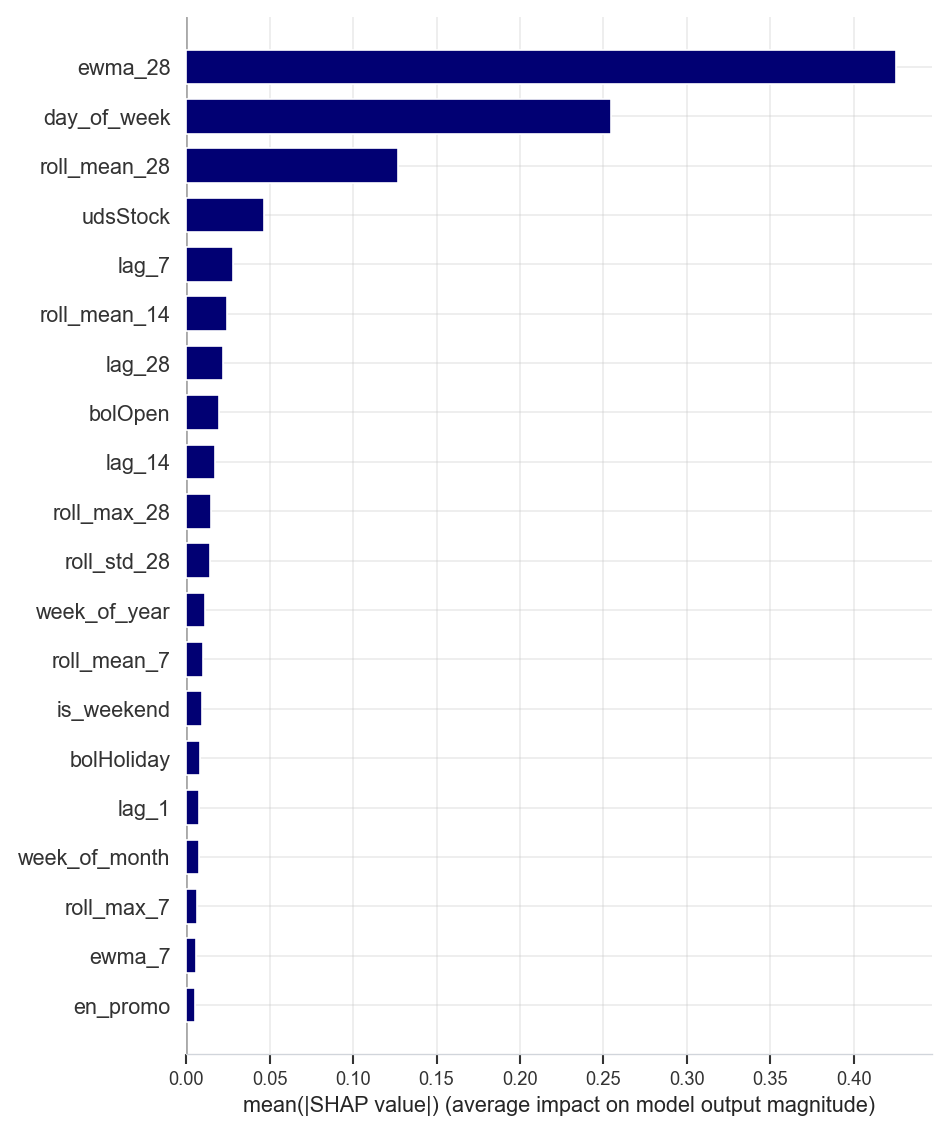
\includegraphics[width=0.85\textwidth]{figures/15_shap_bar.png}
\caption{SHAP feature importance (mean absolute SHAP values) for LightGBM. The 28-day EWMA dominates, followed by calendar and rolling statistics features.}
\label{fig:shap_bar}
\end{figure}

\begin{figure}[H]
\centering
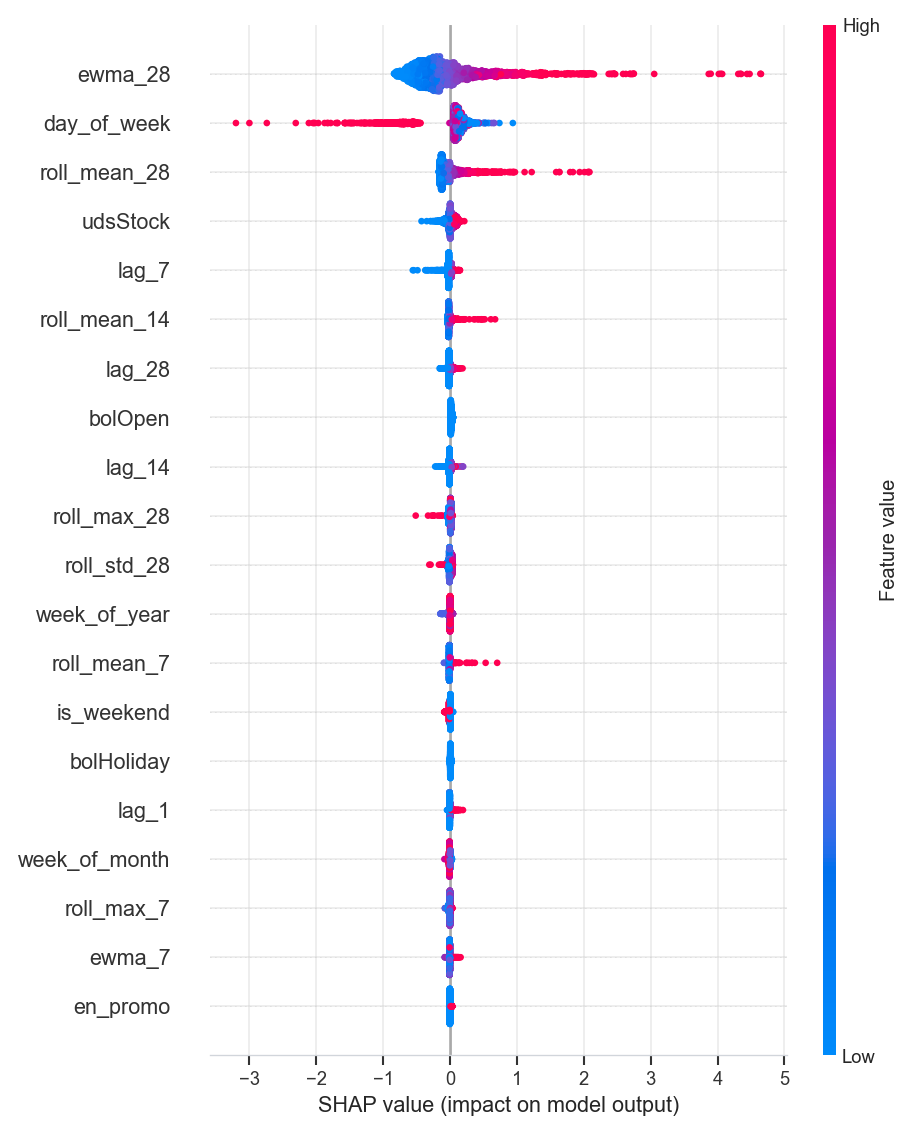
\includegraphics[width=0.85\textwidth]{figures/14_shap_summary.png}
\caption{SHAP summary plot showing the direction and magnitude of feature effects. Red indicates high feature values; blue indicates low values. High \texttt{ewma\_28} values push predictions upward, consistent with higher recent demand leading to higher forecasts.}
\label{fig:shap_summary}
\end{figure}

\subsection{Conclusions from Results}

The evaluation yields several key findings:

\begin{enumerate}
    \item The three tree-based machine learning models (XGBoost, LightGBM, Random Forest) achieve the best performance, with RMSE values within 1\% of each other. This suggests that the feature engineering, rather than the specific algorithm choice, is the primary driver of forecast quality among this model family.

    \item ARIMA and LSTM occupy an intermediate tier, both significantly outperforming the naive baseline (RMSE reductions of 28\% and 28\% respectively) but falling short of the tree-based models. ARIMA's per-product fitting captures local demand patterns effectively but cannot leverage cross-product information or engineered features. LSTM captures sequential dependencies but requires substantially more training data and computation to match tree-based performance.

    \item The improvement over the naive baseline is substantial across all ML approaches (28--30\% RMSE reduction), demonstrating the value of incorporating engineered features and systematic model training over simple heuristic forecasting.

    \item Promotional demand remains the most challenging segment, with RMSE approximately 38\% higher than non-promotional demand across all models. However, the ML models maintain their relative advantage over the baseline in both segments.

    \item SHAP analysis reveals that smoothed demand history (EWMA and rolling statistics) and calendar features are the most influential predictors, validating the feature engineering strategy adopted in this work.

    \item The forecast error standard deviation ($\sigma_e \approx 2.15$ for the best tree models, $\sigma_e \approx 2.22$ for ARIMA/LSTM, compared to $\sigma_e \approx 3.09$ for the naive baseline) translates directly into safety stock reductions, as quantified in the following section.
\end{enumerate}


\section{Impact of Algorithm Improvement}

\subsection{Impact on Processes}

The transition from a naive forecasting approach to machine learning models has implications beyond numerical accuracy improvements. From an operational perspective, the key process impacts are:

\textbf{Safety stock reduction.} Using the safety stock formulation from Equation~\ref{eq:safety_stock} with a 95\% service level ($z = 1.645$) and a protection period of 10 days (3 days lead time + 7 days review period), the total safety stock across all 894 products decreases from 11,953 units under the naive forecast to 8,276 units under LightGBM --- a reduction of 30.8\%. This means that the same service level can be maintained with significantly less inventory investment.

\textbf{Forecast error symmetry.} Analysis of error distributions shows that the ML models produce approximately symmetric errors centred near zero, whereas the naive baseline exhibits a slight positive bias (tendency to overforecast). Symmetric errors are preferable for inventory planning, as they indicate that the forecast is equally likely to overestimate or underestimate demand, allowing safety stock to function as intended.

\textbf{Sensitivity to service level.} Table~\ref{tab:sensitivity} presents the total safety stock requirements across different service levels:

\begin{table}[H]
\centering
\small
\caption{Total safety stock (units) by model and service level.}
\label{tab:sensitivity}
\begin{tabular}{|l|r|r|r|}
\hline
\textbf{Model} & \textbf{90\%} & \textbf{95\%} & \textbf{99\%} \\
\hline
LightGBM & 6,450 & 8,276 & 11,702 \\
XGBoost & 6,466 & 8,296 & 11,731 \\
Random Forest & 6,507 & 8,350 & 11,806 \\
Naive (lag-7) & 9,316 & 11,953 & 16,902 \\
\hline
\end{tabular}
\end{table}

The ML models consistently require approximately 30\% less safety stock than the naive baseline across all service levels, demonstrating that the improvement is robust and not dependent on a specific service level assumption.

\begin{figure}[H]
\centering
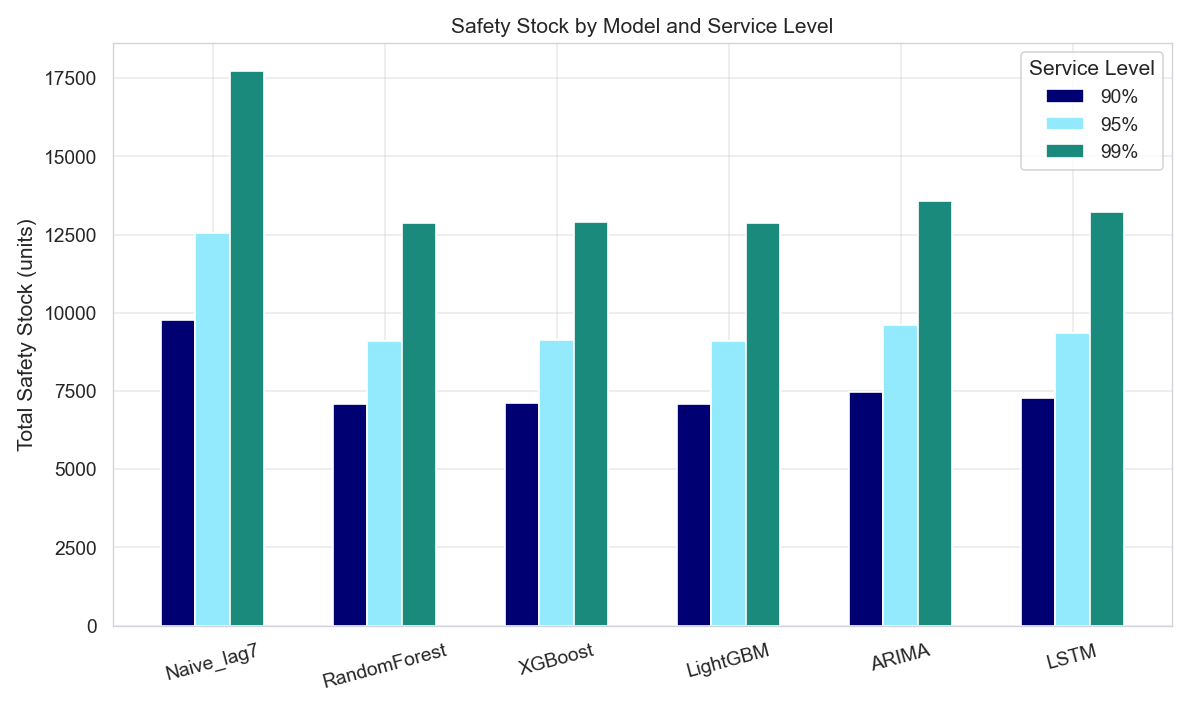
\includegraphics[width=0.85\textwidth]{figures/21_safety_stock_by_service_level.png}
\caption{Total safety stock requirements by model and service level. The ML models maintain a consistent ~30\% advantage over the naive baseline across all service levels.}
\label{fig:safety_stock_service_level}
\end{figure}

\subsection{Economic Impact}

The economic impact analysis combines two cost components: the newsvendor cost (direct cost of forecast errors) and the safety stock holding cost.

\textbf{Newsvendor cost analysis.} Following the total cost formulation from Equation~\ref{eq:total_cost}, the asymmetric costs of overforecasting and underforecasting were computed using cost parameters of $C_o = \text{\euro}0.10$ per unit per day (overage/holding) and $C_u = \text{\euro}0.50$ per unit per day (underage/lost sale), yielding a critical ratio of 0.83. These values reflect a typical retail/industrial setting where stockout costs substantially exceed holding costs.

Table~\ref{tab:newsvendor} presents the newsvendor cost results:

\begin{table}[H]
\centering
\small
\caption{Newsvendor cost analysis (30-day test period, annualised).}
\label{tab:newsvendor}
\begin{tabular}{|l|r|r|r|r|}
\hline
\textbf{Model} & \textbf{Overage (€)} & \textbf{Underage (€)} & \textbf{Total (€)} & \textbf{Annual est. (€)} \\
\hline
Naive (lag-7) & 2,227 & 11,138 & 13,365 & 162,603 \\
Random Forest & 1,830 & 9,538 & 11,367 & 138,304 \\
LightGBM & 1,786 & 9,489 & 11,275 & 137,182 \\
XGBoost & 1,785 & 9,392 & 11,176 & 135,979 \\
\hline
\end{tabular}
\end{table}

XGBoost achieves the lowest newsvendor cost, saving approximately \euro26,600 annually (16.4\%) compared to the naive baseline. Underage costs dominate in all models, consistent with the asymmetric cost structure where stockouts are five times more expensive than excess inventory.

\textbf{Combined cost analysis.} Table~\ref{tab:combined_cost} presents the total annual cost combining newsvendor costs with safety stock holding costs at the 95\% service level:

\begin{table}[H]
\centering
\small
\caption{Combined annual cost: newsvendor + safety stock holding (95\% service level).}
\label{tab:combined_cost}
\begin{tabular}{|l|r|r|r|}
\hline
\textbf{Model} & \textbf{Newsvendor (€/yr)} & \textbf{SS Holding (€/yr)} & \textbf{Total (€/yr)} \\
\hline
Naive (lag-7) & 162,603 & 436,294 & 598,896 \\
Random Forest & 138,304 & 304,763 & 443,067 \\
LightGBM & 137,182 & 302,083 & 439,265 \\
XGBoost & 135,979 & 302,816 & 438,796 \\
\hline
\end{tabular}
\end{table}

The ML models achieve total annual cost savings of approximately \euro160,000 (26.7\%) compared to the naive baseline. XGBoost and LightGBM perform nearly identically in economic terms, with XGBoost holding a marginal advantage of \euro469 annually.

\begin{figure}[H]
\centering
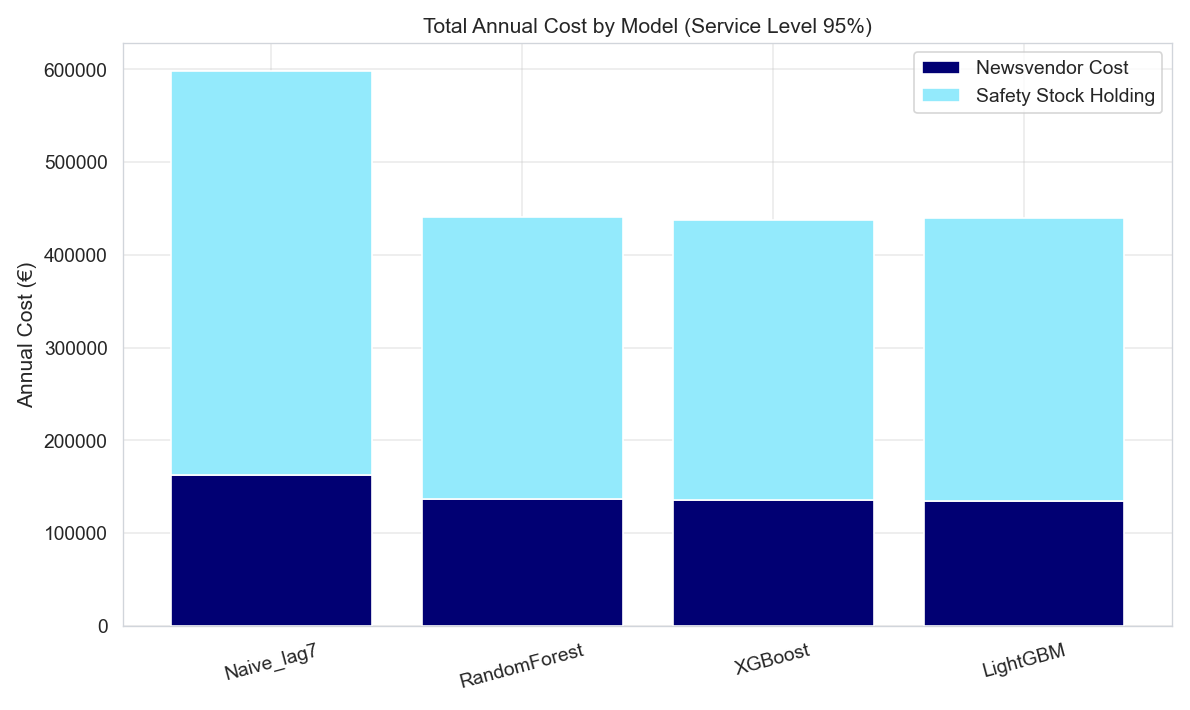
\includegraphics[width=0.85\textwidth]{figures/22_combined_annual_cost.png}
\caption{Combined annual inventory cost (newsvendor + safety stock holding) by model. The ML models reduce total costs by approximately 26.7\% compared to the naive baseline.}
\label{fig:combined_annual_cost}
\end{figure}

These results demonstrate that the forecast accuracy improvements documented in Section~3.6 translate into meaningful economic benefits. The 28\% reduction in RMSE corresponds to a 26.7\% reduction in total inventory-related costs, confirming the theoretical relationship between forecast error and inventory costs established in Chapter~2 (Equations~\ref{eq:ss_cost} and \ref{eq:total_cost}).

It is important to note that the cost parameters used in this analysis ($C_o$ and $C_u$) are illustrative values chosen to reflect typical industrial cost structures. The relative ranking of models and the percentage savings are robust to reasonable variations in these parameters, as the underlying driver is the reduction in forecast error rather than the specific cost assumptions. A sensitivity analysis across service levels (Table~\ref{tab:sensitivity}) confirms that the ML advantage is maintained regardless of the risk tolerance adopted by the organisation.
 in TFM_onamas.tex

This chapter presents the complete design and implementation of the demand forecasting system, following the CRISP-DM methodology introduced in Chapter~1. The work progresses from data acquisition and exploration through preprocessing, feature engineering, model development, evaluation, and finally the economic impact analysis that connects forecast accuracy to inventory cost savings.

\section{Data Origin}

\subsection{Data Acquisition}

The dataset used in this project was provided by the thesis supervisor and corresponds to real historical data from a company operating in the automotive sector. The data covers daily demand records for a portfolio of products, along with supplementary information on calendar events, promotional campaigns, and stock levels. All data was received in a single Microsoft Excel file (\texttt{Datos.xlsx}) containing four sheets, each representing a distinct dimension of the business context.

No personally identifiable information is present in the dataset, and all product references are anonymised using numerical identifiers, ensuring compliance with data privacy requirements as discussed in Section~\ref{s:etic}.

\subsection{Data Description}

The dataset comprises four tables, summarised in Table~\ref{tab:data_sheets}:

\begin{table}[H]
\centering
\small
\caption{Structure of the source dataset (\texttt{Datos.xlsx}).}
\label{tab:data_sheets}
\begin{tabular}{|l|l|r|p{5.5cm}|}
\hline
\textbf{Sheet} & \textbf{Key columns} & \textbf{Rows} & \textbf{Description} \\
\hline
Ventas (Sales) & producto, fecha, udsVenta & 654,588 & Daily unit sales per product \\
\hline
Calendario & fecha, bolOpen, bolHoliday & 732 & Calendar flags: business day and holiday indicators \\
\hline
Promociones & producto, fechaInicio, fechaFin & 1,894 & Promotional campaign periods per product \\
\hline
Stock & producto, fecha, udsStock & 654,588 & Daily stock levels per product \\
\hline
\end{tabular}
\end{table}

The sales sheet constitutes the core of the dataset, containing 654,588 daily observations across 894 unique products over a period of 732 days, spanning from November 2022 to November 2024. Each record represents the number of units sold for a specific product on a specific date.

The calendar sheet provides 732 daily records with two binary indicators: \texttt{bolOpen} (whether the business was open) and \texttt{bolHoliday} (whether the date was a public holiday). The promotions sheet contains 1,894 records defining promotional campaign windows through start and end dates for each product. The stock sheet mirrors the sales structure, recording the closing stock level for each product-date combination.

\subsection{Data Loading}

All four sheets were loaded into memory using the \texttt{pandas} library with the \texttt{openpyxl} engine. The sales and stock tables were merged on the shared keys \texttt{(producto, fecha)}, and the calendar information was joined on \texttt{fecha}. Promotional periods were transformed from date ranges into a binary indicator (\texttt{en\_promo}) at the product-date level, marking each observation as promotional or non-promotional based on whether the date fell within any active campaign for that product.

After merging, the resulting dataset contained 654,588 rows and served as the foundation for all subsequent analysis. The merged dataset was persisted in Apache Parquet format for efficient reloading in downstream scripts.


\section{Data Exploration}

\subsection{Data Summary}

An initial statistical summary of the target variable (\texttt{udsVenta}, units sold) revealed a highly skewed distribution. The mean daily sales per product were 1.42 units, with a median of zero and a standard deviation of 3.56. The maximum observed value was 99 units. This distribution reflects the nature of automotive parts demand, where the majority of product-day combinations register zero sales, punctuated by occasional larger orders.

Table~\ref{tab:sales_stats} presents the key descriptive statistics:

\begin{table}[H]
\centering
\small
\caption{Descriptive statistics of daily unit sales (\texttt{udsVenta}).}
\label{tab:sales_stats}
\begin{tabular}{|l|r|}
\hline
\textbf{Statistic} & \textbf{Value} \\
\hline
Count & 654,588 \\
Mean & 1.42 \\
Std. deviation & 3.56 \\
Median (50\%) & 0.00 \\
75th percentile & 1.00 \\
95th percentile & 7.00 \\
Maximum & 99 \\
Zero-sales proportion & 64.5\% \\
\hline
\end{tabular}
\end{table}

The high proportion of zero-sales observations (64.5\%) is a defining characteristic of this dataset and has important implications for model selection and evaluation, as discussed in subsequent sections.

\begin{figure}[H]
\centering
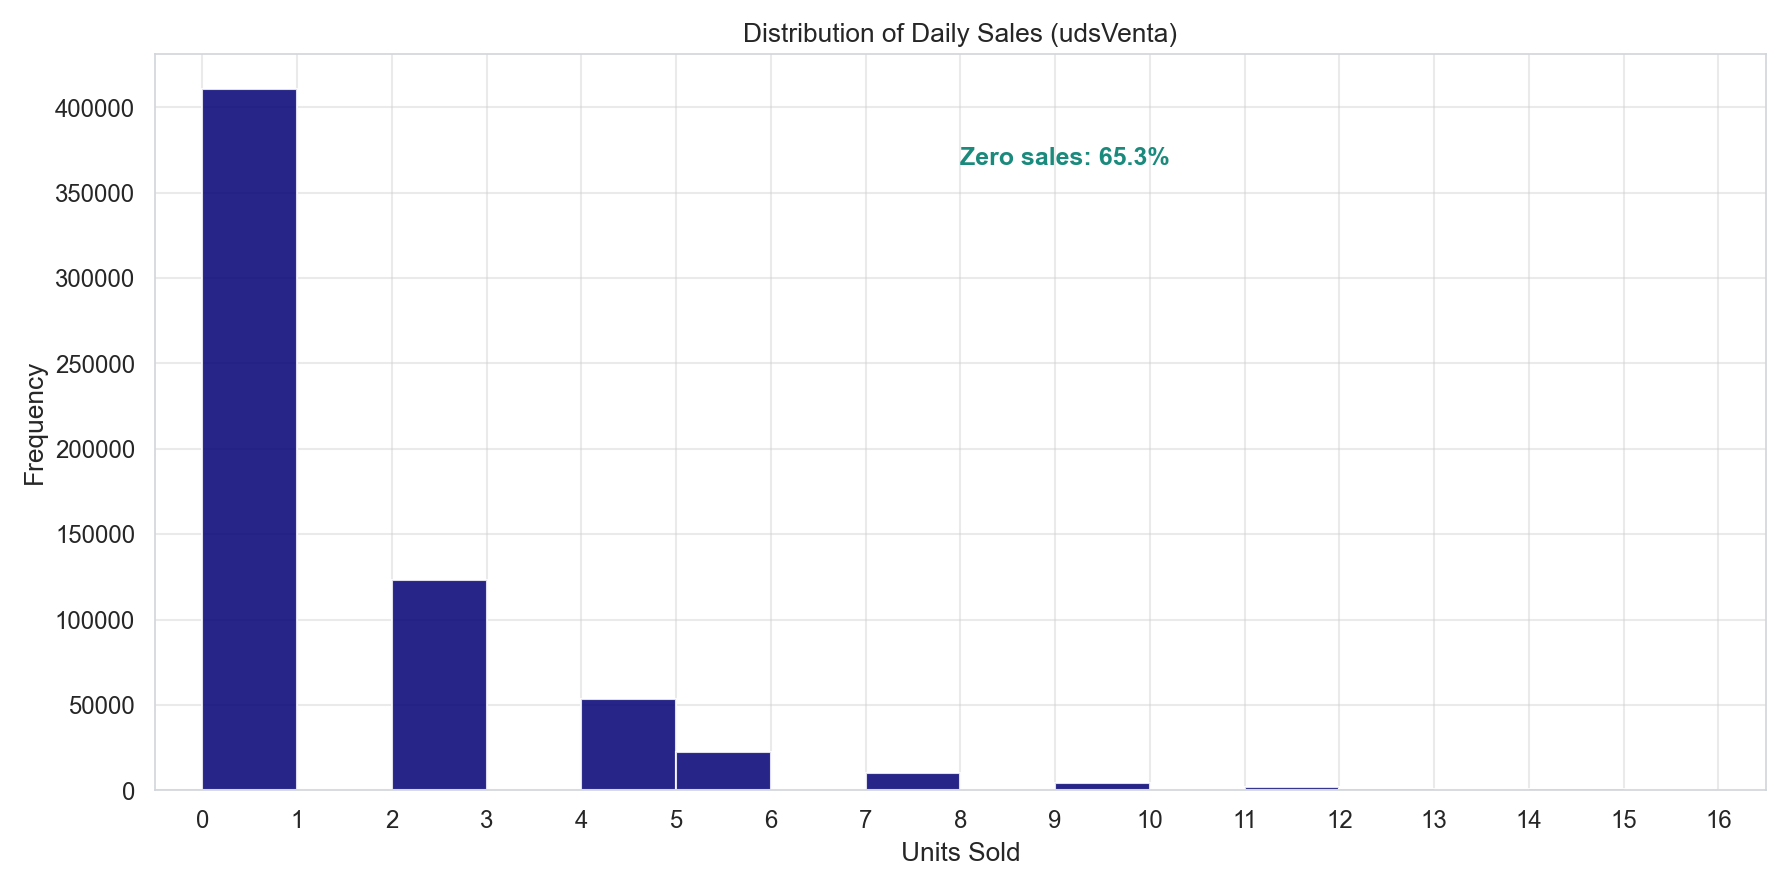
\includegraphics[width=0.85\textwidth]{figures/01_sales_distribution.png}
\caption{Distribution of daily unit sales (\texttt{udsVenta}). The histogram confirms the extreme right skew, with the majority of observations at zero.}
\label{fig:sales_distribution}
\end{figure}

\subsection{Statistical Analysis}

The exploratory analysis examined demand patterns across several dimensions:

\textbf{Day-of-week patterns.} Sales exhibit a clear weekly cycle, with the highest volumes on weekdays (Monday through Friday) and a sharp decline on Saturdays. Sunday sales are near zero, consistent with the business being closed on Sundays as indicated by the \texttt{bolOpen} calendar flag. This weekly seasonality motivates the inclusion of day-of-week features and the use of a lag-7 naive baseline (same weekday, previous week) as the primary benchmark.

\begin{figure}[H]
\centering
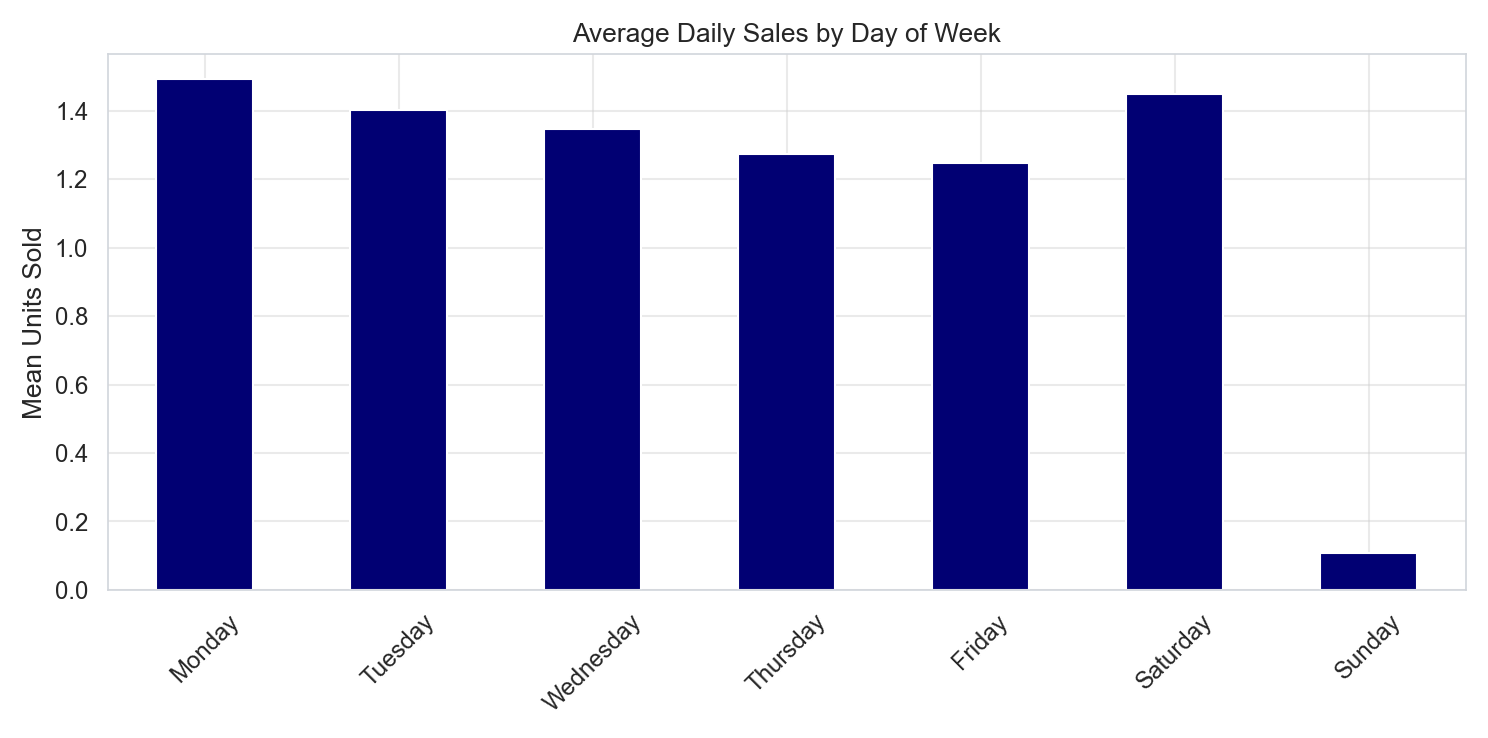
\includegraphics[width=0.85\textwidth]{figures/02_sales_by_day_of_week.png}
\caption{Average daily sales by day of the week. The weekly cycle is clearly visible, with near-zero sales on Sundays.}
\label{fig:sales_by_dow}
\end{figure}

\textbf{Monthly and seasonal patterns.} Monthly aggregated sales show moderate variation across the year, without a single dominant seasonal peak. However, certain months consistently show higher activity, suggesting that calendar-based features (month, week of year) may contribute predictive value.

\textbf{Promotional effects.} Comparing sales during promotional and non-promotional periods revealed that mean sales during promotions (1.83 units) were slightly higher than during non-promotional periods (1.38 units). However, the difference is modest, and the promotional flag alone does not capture the full complexity of promotional demand dynamics, which motivated the engineering of additional promotional features described in Section~3.4.

\begin{figure}[H]
\centering
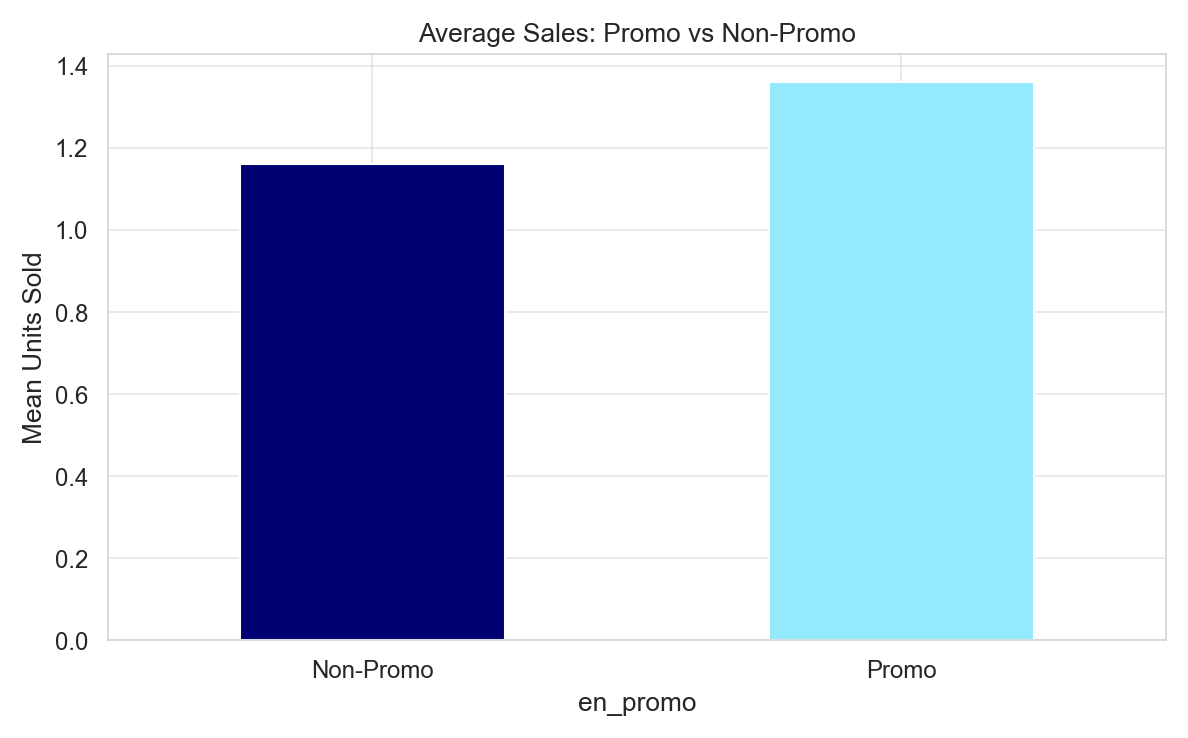
\includegraphics[width=0.85\textwidth]{figures/05_promo_vs_nonpromo.png}
\caption{Comparison of sales distributions during promotional and non-promotional periods.}
\label{fig:promo_vs_nonpromo}
\end{figure}

\textbf{Autocorrelation structure.} Autocorrelation analysis on a sample of products confirmed significant positive autocorrelation at lags 1, 7, 14, and 28, with the strongest signal at lag 7 (weekly periodicity). This finding directly supports the creation of lag features at these intervals and validates the choice of lag-7 as the naive baseline.

\begin{figure}[H]
\centering
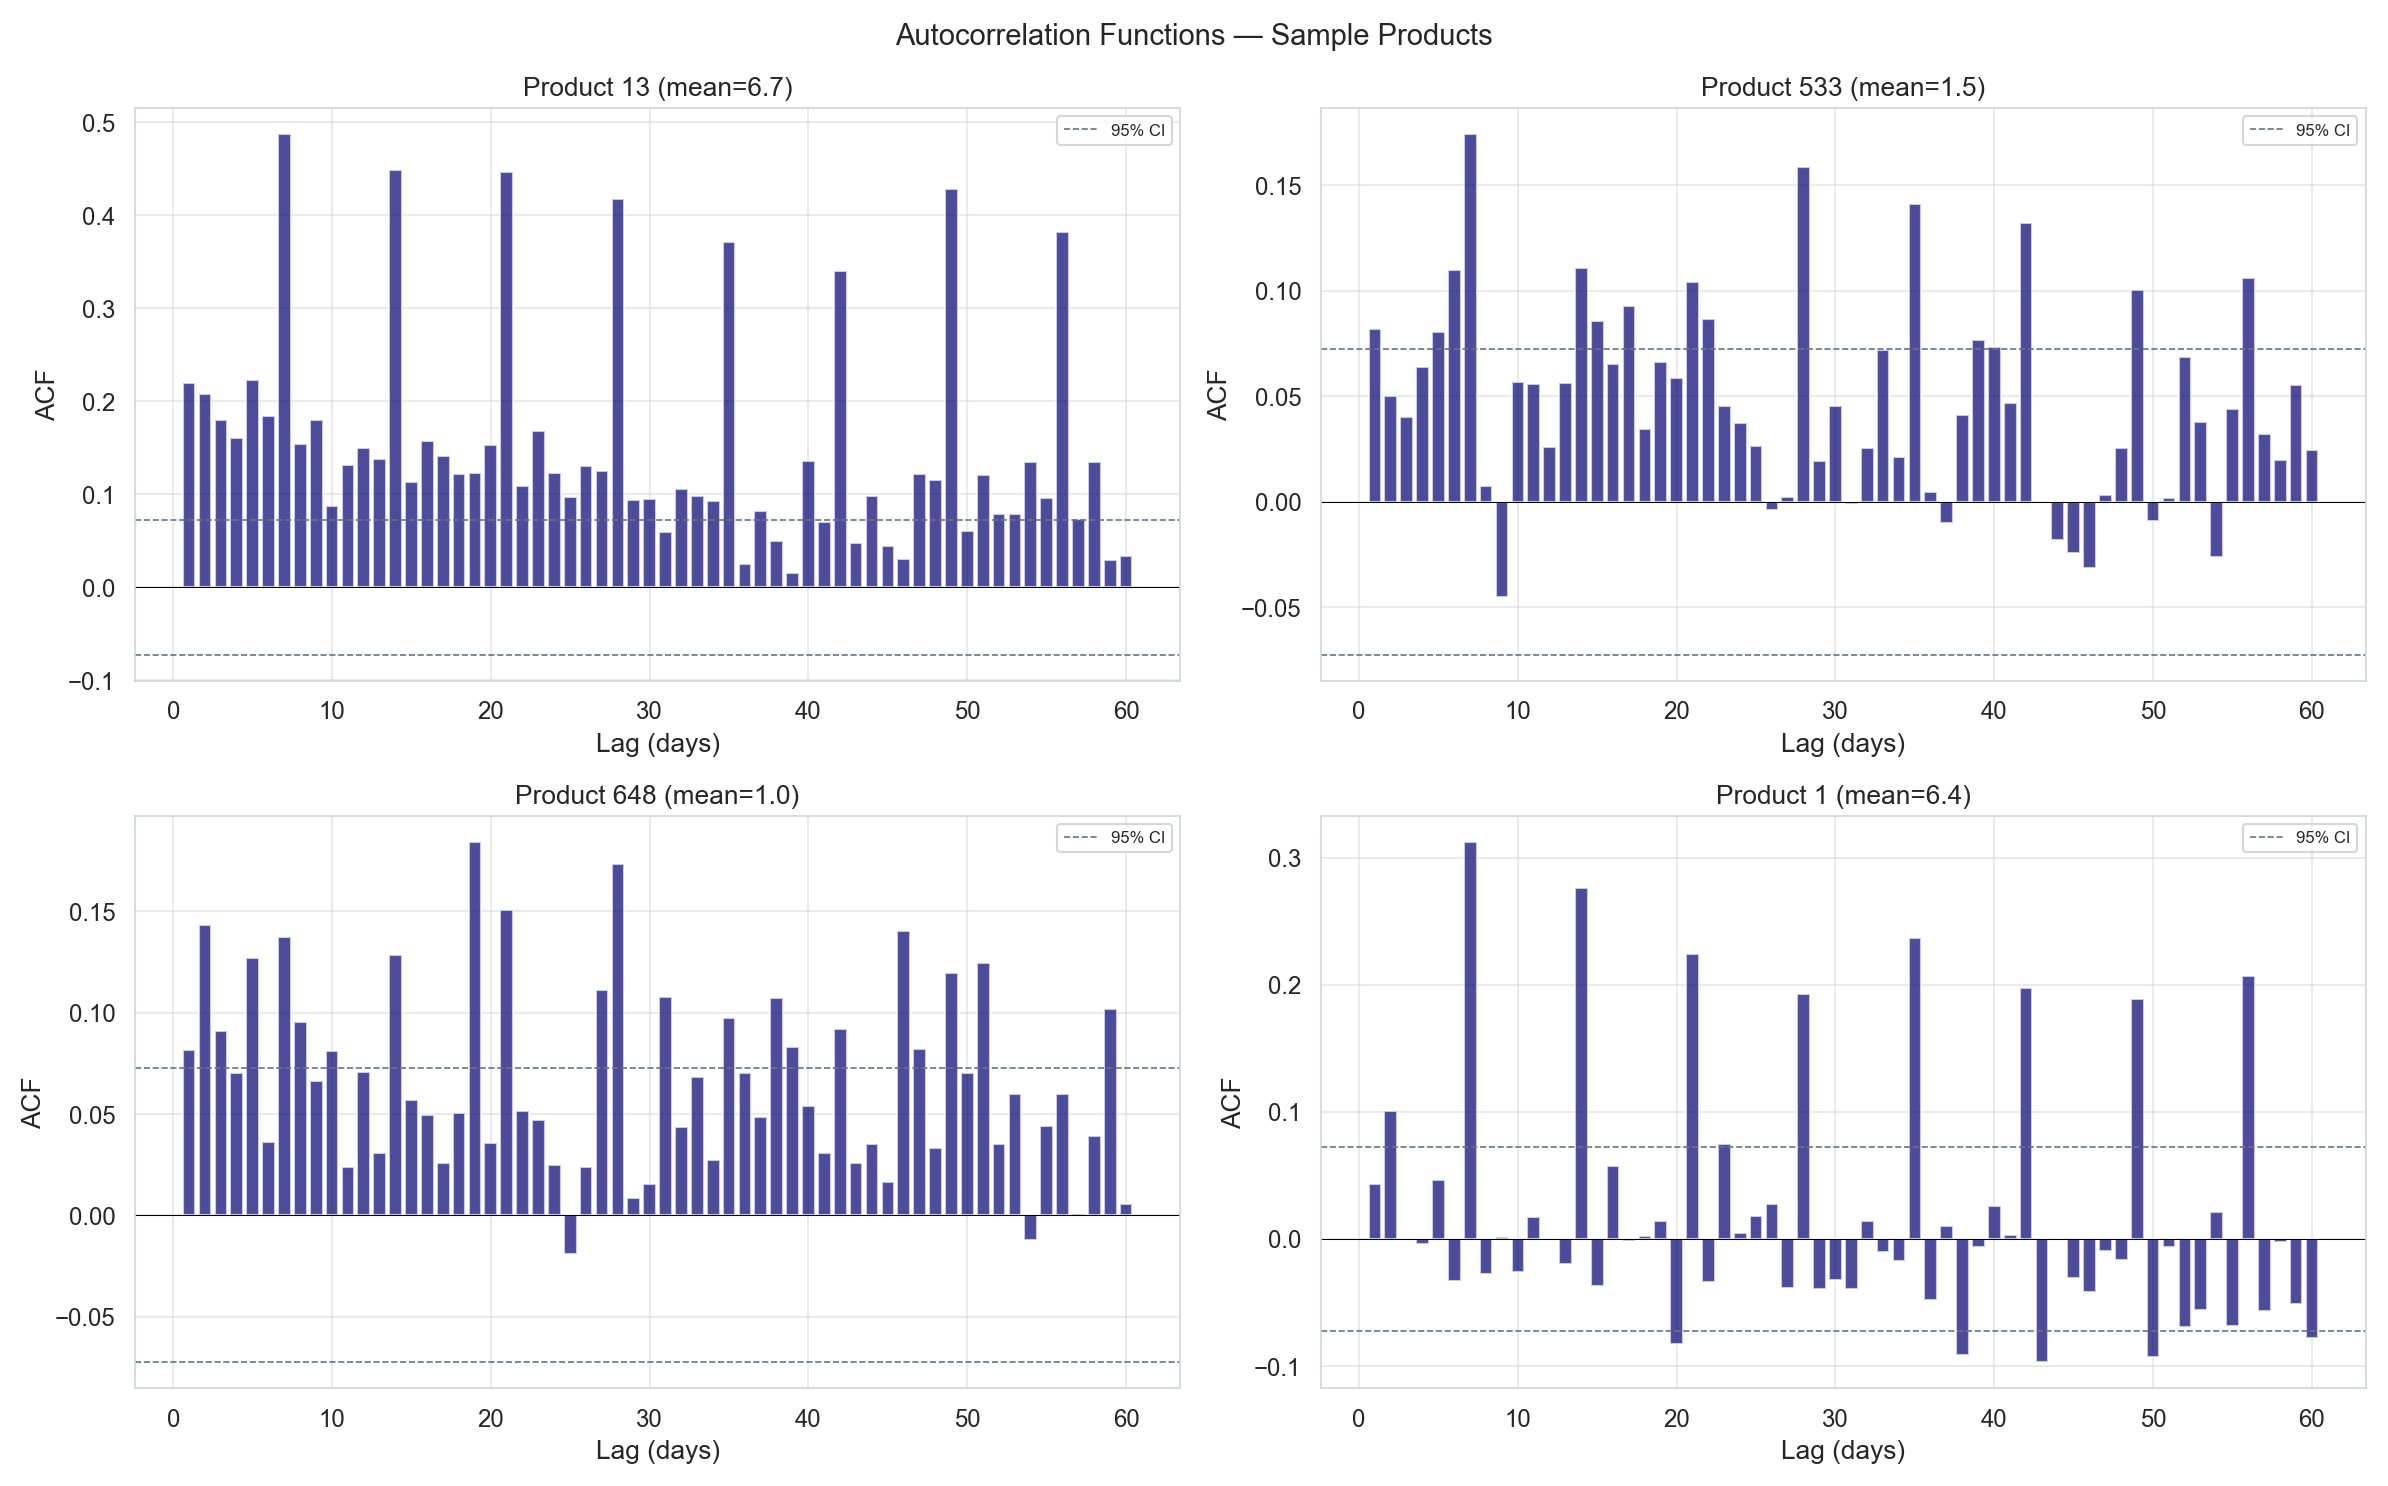
\includegraphics[width=0.85\textwidth]{figures/08_autocorrelation_sample.png}
\caption{Autocorrelation function (ACF) for a sample of products, showing significant positive autocorrelation at weekly intervals.}
\label{fig:autocorrelation}
\end{figure}

\subsection{Data Quality Analysis}

The data quality assessment identified the following issues:

\textbf{Missing values.} No explicit missing values were found in any of the four source tables. However, implicit gaps exist where lag features cannot be computed for the earliest dates in each product's history (addressed during feature engineering).

\textbf{Negative values.} No negative sales or stock values were present in this dataset.

\textbf{Stock breaks.} A stock break is defined as a day where both sales and stock are zero, potentially indicating that demand existed but could not be fulfilled due to inventory unavailability. Approximately 3.9\% of observations met this criterion. These were treated during data cleaning by imputing the product's historical mean sales for the corresponding weekday.

\textbf{Outliers.} Outlier detection was performed using a threshold of 1.75 times the interquartile range (IQR) per product. This identified approximately 11,400 observations (1.75\% of the dataset) as outliers, which were capped at the upper threshold value. The IQR-based approach was preferred over a fixed standard deviation threshold to account for the varying demand scales across products.


\section{Data Preparation}

\subsection{Data Cleaning}

The data cleaning process addressed the two quality issues identified during exploration:

\begin{enumerate}
    \item \textbf{Stock break imputation:} For observations where both \texttt{udsVenta} and \texttt{udsStock} were zero, the sales value was replaced with the mean sales for that product on the same weekday, computed over the preceding 30 days. This approach assumes that zero sales on a day with zero stock reflects a supply-side constraint rather than genuine zero demand, and uses a localised historical average to provide a reasonable demand estimate.

    \item \textbf{Outlier capping:} Values exceeding 1.75 $\times$ IQR above the 75th percentile for each product were capped at the threshold value. This preserves the general distribution shape while limiting the influence of extreme observations on model training. A total of 11,400 values (1.75\% of the dataset) were capped.
\end{enumerate}

After cleaning, the dataset retained its original 654,588 rows with no records removed, ensuring that the temporal continuity required for lag feature computation was preserved.

\subsection{Data Transformation}

The date column (\texttt{fecha}) was parsed into a \texttt{datetime} type, and the dataset was sorted by product and date to ensure correct temporal ordering for all subsequent operations. The promotional periods from the source data were transformed from date-range format into a daily binary indicator (\texttt{en\_promo}), assigned at the product-date level.

No logarithmic or power transformations were applied to the target variable. While such transformations can stabilise variance in skewed distributions, the tree-based models used in this work (Random Forest, XGBoost, LightGBM) are inherently robust to non-normal distributions and do not require target transformation for effective learning.

\subsection{Data Scaling}

Feature scaling (standardisation or normalisation) was not applied for the tree-based models, as decision tree ensembles are invariant to monotonic transformations of input features. The split-based learning mechanism of these algorithms operates on feature rankings rather than absolute values, making scaling unnecessary.

For the LSTM model, min-max normalisation was applied to all input features to facilitate gradient-based optimisation. Each feature was scaled to the $[0, 1]$ range using the training set statistics, and the same transformation was applied to the validation and test sets to prevent information leakage. Predictions were inverse-transformed back to the original scale before computing evaluation metrics.

\section{Feature Engineering}

Feature engineering is a central component of this work. A comprehensive set of 36 engineered features was designed to capture temporal dependencies, demand dynamics, and promotional effects. The features are organised into five categories, summarised in Table~\ref{tab:features}.

\begin{table}[H]
\centering
\small
\caption{Engineered features by category.}
\label{tab:features}
\begin{tabular}{|l|p{7cm}|r|}
\hline
\textbf{Category} & \textbf{Features} & \textbf{Count} \\
\hline
Original variables & udsStock, bolOpen, bolHoliday, en\_promo & 4 \\
\hline
Calendar features & year, month, day\_of\_week, week\_of\_year, week\_of\_month, is\_weekend, is\_month\_start, is\_month\_end & 8 \\
\hline
Lag features & lag\_1, lag\_7, lag\_14, lag\_28 & 4 \\
\hline
Rolling statistics & roll\_mean/std/min/max at 7, 14, and 28-day windows; ewma\_7, ewma\_28 & 14 \\
\hline
Promotional features & days\_since\_promo\_end, post\_promo\_7d, promo\_x\_lag7 & 3 \\
\hline
Product-level statistics & prod\_mean\_sales, prod\_std\_sales, prod\_median\_sales & 3 \\
\hline
\multicolumn{2}{|r|}{\textbf{Total}} & \textbf{36} \\
\hline
\end{tabular}
\end{table}

\textbf{Lag features} capture the autoregressive structure identified during exploration. The lag-7 feature (same weekday, previous week) serves dual purpose: it is used directly as the naive baseline forecast and as an input feature for the machine learning models. Lags at 1, 14, and 28 days capture short-term momentum, biweekly patterns, and monthly cycles respectively.

\textbf{Rolling statistics} provide smoothed representations of recent demand behaviour. For each window size (7, 14, and 28 days), the mean, standard deviation, minimum, and maximum of past sales are computed. Additionally, exponentially weighted moving averages (EWMA) with spans of 7 and 28 days provide adaptive smoothing that gives greater weight to more recent observations.

\textbf{Promotional features} go beyond the binary indicator to capture the temporal dynamics of promotions. The \texttt{days\_since\_promo\_end} feature tracks the recency of the last promotional period, \texttt{post\_promo\_7d} flags the week immediately following a promotion (to capture post-promotional demand depression), and \texttt{promo\_x\_lag7} is an interaction term between the promotional flag and the lag-7 sales value.

All lag and rolling features were computed strictly using past data to prevent information leakage. Observations where lag features could not be computed (the first 28 days of each product's history) were dropped, reducing the dataset from 654,588 to 629,370 rows. The final feature matrix was saved in Parquet format for use in the modelling phase.

\begin{figure}[H]
\centering
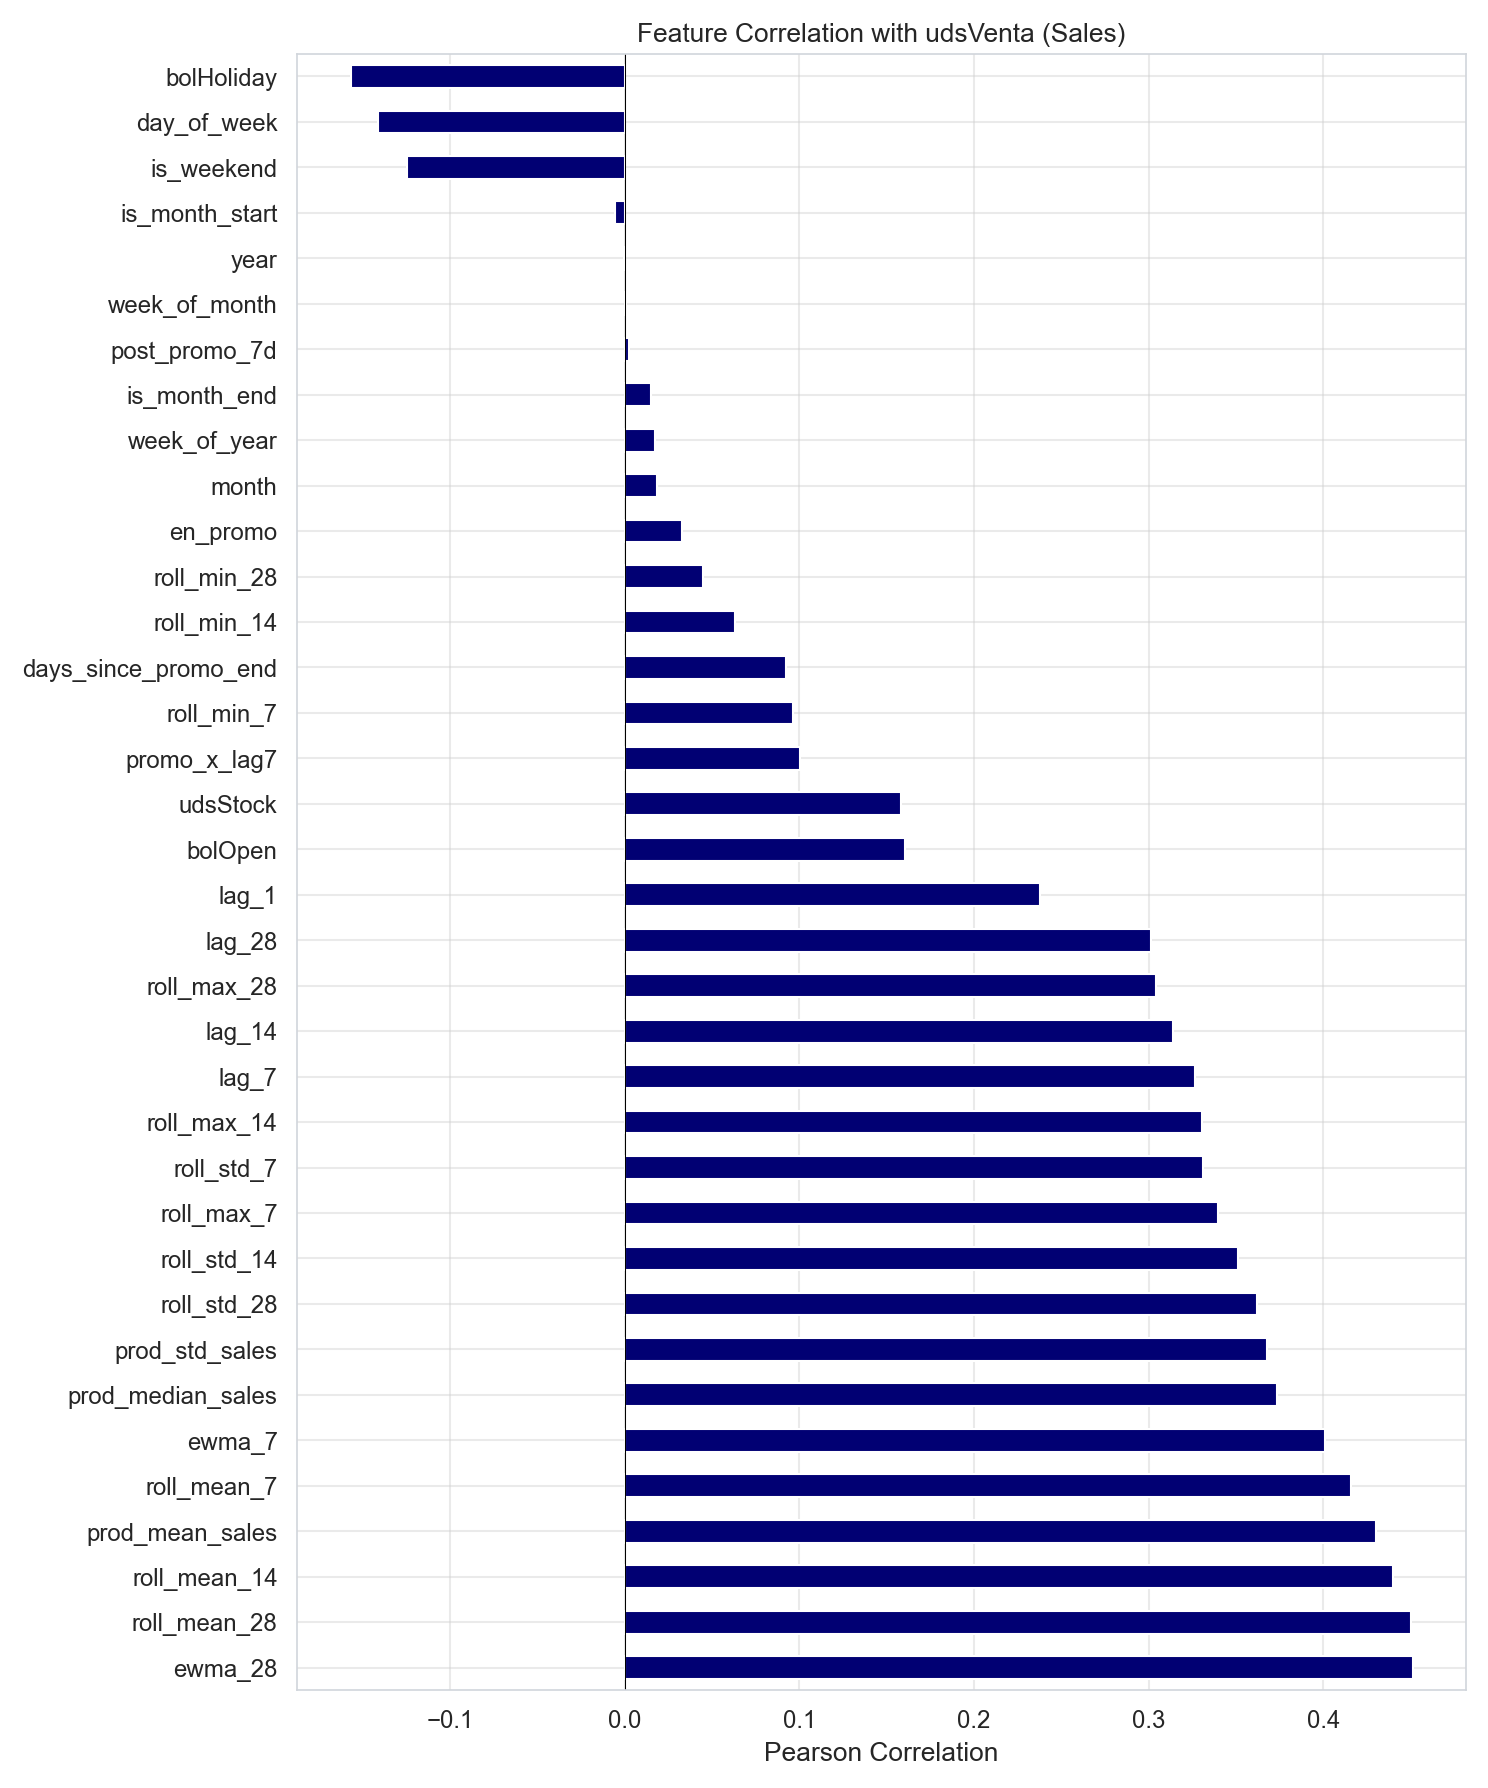
\includegraphics[width=0.95\textwidth]{figures/10_feature_correlations.png}
\caption{Correlation matrix of the engineered features. Strong correlations are visible among rolling statistics at different window sizes, confirming the presence of redundant but complementary temporal signals.}
\label{fig:feature_correlations}
\end{figure}


\section{Modelling}

\subsection{Model Selection}

Four forecasting approaches were implemented, spanning a naive baseline and three gradient boosting / ensemble methods:

\begin{enumerate}
    \item \textbf{Naive baseline (lag-7):} The simplest possible forecast, predicting that demand on any given day equals the demand observed on the same weekday of the previous week. This baseline exploits the strong weekly autocorrelation identified during exploration and provides a meaningful benchmark against which machine learning models must demonstrate improvement.

    \item \textbf{ARIMA (Seasonal):} A classical time series approach fitted per product using the \texttt{auto\_arima} implementation from the \texttt{pmdarima} library. Each product's demand series was modelled with seasonal ARIMA (SARIMA) with weekly periodicity ($m=7$), automatically selecting the optimal $(p,d,q)(P,D,Q)_7$ orders via stepwise search. ARIMA serves as the classical statistical baseline, representing the best that traditional time series methods can achieve without engineered features.

    \item \textbf{Random Forest:} An ensemble of decision trees trained on bootstrap samples with random feature subsets \citep{hyndman2021forecasting}. Random Forest provides robust predictions with built-in protection against overfitting through bagging and feature randomisation.

    \item \textbf{XGBoost:} A gradient boosting framework that builds trees sequentially, with each tree correcting the errors of its predecessors. XGBoost incorporates L1 and L2 regularisation, column subsampling, and efficient handling of sparse data, making it well-suited to the high proportion of zero-demand observations in this dataset.

    \item \textbf{LightGBM:} A gradient boosting implementation that uses histogram-based splitting and leaf-wise tree growth, offering faster training times than XGBoost while maintaining competitive accuracy. LightGBM was among the dominant algorithms in the M5 forecasting competition \citep{makridakis2021m5findings}.

    \item \textbf{LSTM (Long Short-Term Memory):} A recurrent neural network architecture designed to capture long-range temporal dependencies in sequential data \citep{hochreiter1997lstm}. Unlike tree-based methods, which rely on engineered lag features, LSTM processes input data as ordered sequences, with its internal gating mechanism allowing it to selectively retain or discard information from previous time steps. The model was implemented in PyTorch with a single LSTM layer (32 hidden units), trained on standardised features using 14-day input sequences.
\end{enumerate}

All tree-based models were trained on the full set of 33 input features (the 36 engineered features minus the 3 product-level statistics used only for reference). ARIMA was fitted per product on the raw sales series without engineered features, as is standard for classical time series methods. The LSTM model received the same 33 features as the tree models, but processed them as ordered sequences rather than independent observations. All predictions were clipped to a minimum of zero to prevent negative forecast values.

\subsection{Definition of Accuracy Indicators}

Four complementary metrics were used to evaluate forecast performance, as introduced in Chapter~2:

\begin{itemize}
    \item \textbf{MAE} (Mean Absolute Error): average absolute deviation between forecast and actual demand, in the same units as the target variable.
    \item \textbf{RMSE} (Root Mean Squared Error): penalises larger errors more heavily than MAE, providing a measure sensitive to occasional large deviations.
    \item \textbf{MAPE} (Mean Absolute Percentage Error): expresses errors as a percentage of actual demand, computed only for observations where actual demand is greater than zero to avoid division by zero.
    \item \textbf{$\sigma_e$} (forecast error standard deviation): the standard deviation of the residuals ($D_t - F_t$), which directly enters the safety stock calculation (Equation~\ref{eq:safety_stock}) and thus provides the link between forecast accuracy and inventory cost.
\end{itemize}

\subsection{Definition of Training and Validation Periods}

A rolling forecast origin validation strategy was adopted to provide a realistic assessment of out-of-sample performance by simulating the sequential nature of real forecasting decisions \citep{makridakis2021m5findings}.

Three validation folds were defined, each with a 30-day test window, working backwards from the most recent date in the dataset:

\begin{table}[H]
\centering
\small
\caption{Rolling forecast origin validation folds.}
\label{tab:folds}
\begin{tabular}{|c|c|c|c|}
\hline
\textbf{Fold} & \textbf{Training period end} & \textbf{Test period} & \textbf{Test days} \\
\hline
1 & 2024-09-06 & 2024-09-07 -- 2024-10-06 & 30 \\
2 & 2024-10-06 & 2024-10-07 -- 2024-11-05 & 30 \\
3 & 2024-10-06 & 2024-10-07 -- 2024-11-05 & 30 \\
\hline
\end{tabular}
\end{table}

For each fold, the training set includes all data up to the fold's cutoff date (expanding window), and the model is evaluated on the subsequent 30-day period. Final reported metrics are averaged across all three folds.

\subsection{Hyperparameter Tuning}

Hyperparameters for all three machine learning models were optimised using Optuna \citep{makridakis2021m5findings}, a Bayesian optimisation framework that efficiently explores the parameter space using a Tree-structured Parzen Estimator (TPE) sampler.

To balance computational cost with tuning quality, the optimisation was conducted on a representative subset of 50 randomly sampled products using the first validation fold. Each model was allocated 30 Optuna trials, with RMSE on the validation set as the objective function. The optimised hyperparameters were then applied to the full dataset across all validation folds.

Table~\ref{tab:tuned_params} presents the key tuned hyperparameters for each model:

\begin{table}[H]
\centering
\small
\caption{Optimised hyperparameters via Optuna (30 trials per model).}
\label{tab:tuned_params}
\begin{tabular}{|l|l|r|}
\hline
\textbf{Model} & \textbf{Parameter} & \textbf{Value} \\
\hline
\multirow{5}{*}{LightGBM} & n\_estimators & 300 \\
 & learning\_rate & 0.011 \\
 & num\_leaves & 75 \\
 & max\_depth & 4 \\
 & min\_child\_samples & 25 \\
\hline
\multirow{5}{*}{XGBoost} & n\_estimators & 350 \\
 & learning\_rate & 0.019 \\
 & max\_depth & 3 \\
 & min\_child\_weight & 10 \\
 & subsample & 0.90 \\
\hline
\multirow{4}{*}{Random Forest} & n\_estimators & 100 \\
 & max\_depth & 5 \\
 & min\_samples\_leaf & 16 \\
 & max\_features & 0.30 \\
\hline
\end{tabular}
\end{table}

The relatively shallow tree depths (3--5) and conservative learning rates (0.011--0.019) selected by the optimiser suggest that the models benefit from regularisation, which is consistent with the high proportion of zero-demand observations in the dataset.


\section{Evaluation}

\subsection{Accuracy Results Obtained}

Table~\ref{tab:results_summary} presents the average performance of each model across the three validation folds:

\begin{table}[H]
\centering
\small
\caption{Average forecast accuracy across three rolling validation folds.}
\label{tab:results_summary}
\begin{tabular}{|l|r|r|r|r|}
\hline
\textbf{Model} & \textbf{MAE} & \textbf{RMSE} & \textbf{MAPE (\%)} & \textbf{$\sigma_e$} \\
\hline
XGBoost & 1.366 & 2.155 & 52.2 & 2.154 \\
LightGBM & 1.373 & 2.158 & 51.7 & 2.158 \\
Random Forest & 1.394 & 2.176 & 51.6 & 2.176 \\
ARIMA$^\dagger$ & 1.443 & 2.220 & 59.8 & 2.219 \\
LSTM & 1.522 & 2.235 & 49.8 & 2.223 \\
Naive (lag-7) & 1.661 & 3.091 & 86.0 & 3.091 \\
\hline
\end{tabular}
\begin{flushleft}
\footnotesize{$^\dagger$ ARIMA evaluated on 50 sampled products due to per-product fitting cost.}
\end{flushleft}
\end{table}

All three tree-based machine learning models substantially outperform both the naive baseline and the classical/deep learning alternatives. XGBoost achieves the lowest RMSE (2.155), followed closely by LightGBM (2.158) and Random Forest (2.176). The RMSE improvement over the naive baseline ranges from 27.9\% (LSTM) to 30.3\% (XGBoost).

\begin{figure}[H]
\centering
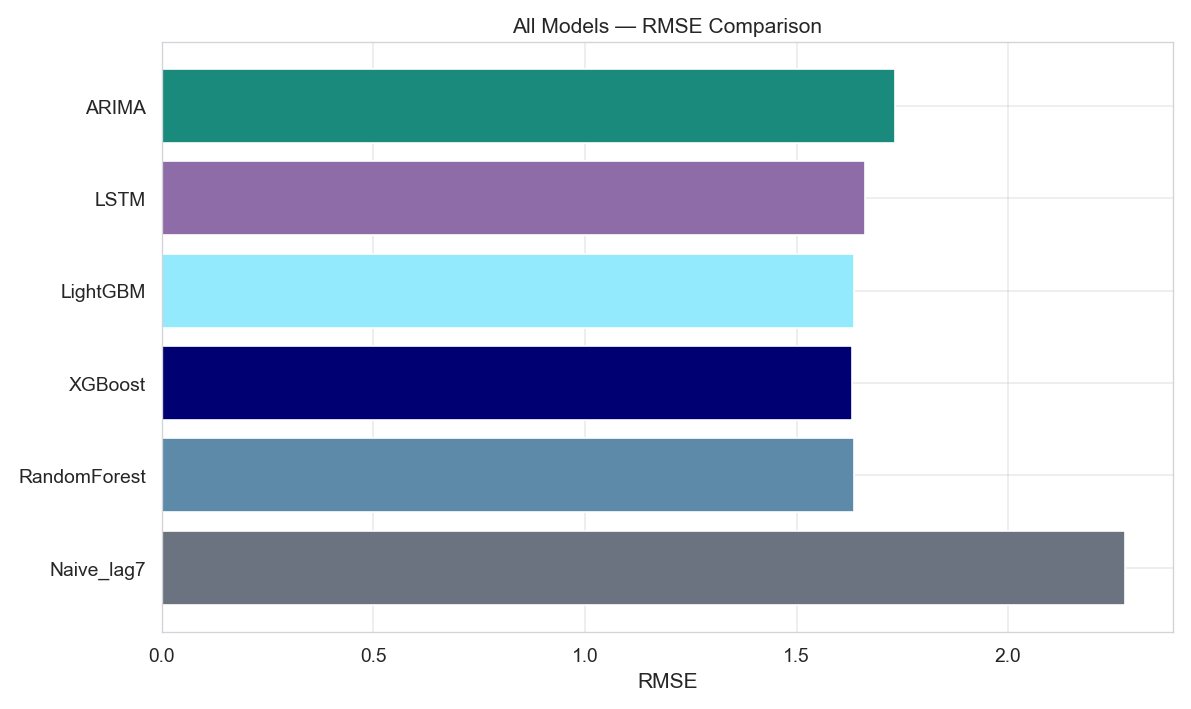
\includegraphics[width=0.85\textwidth]{figures/24_all_models_comparison.png}
\caption{Comparison of forecast accuracy (RMSE) across all six models. The three tree-based models form a tight cluster, substantially outperforming both classical and deep learning alternatives.}
\label{fig:all_models_comparison}
\end{figure}

ARIMA and LSTM occupy an intermediate position: both significantly outperform the naive baseline (RMSE reductions of 28.2\% and 27.7\% respectively) but fall short of the tree-based models. This result is consistent with the findings of the M5 forecasting competition \citep{makridakis2021m5findings}, where gradient boosting algorithms consistently outperformed both classical statistical methods and standalone deep learning approaches. The LSTM's slightly lower MAPE (49.8\%) but higher RMSE suggests it handles the zero-heavy distribution differently from tree models, producing fewer large percentage errors but occasionally larger absolute deviations.

\subsection{Comparison of Results Across Models}

\textbf{Promotional vs. non-promotional performance.} Table~\ref{tab:promo_results} compares model performance across demand segments:

\begin{table}[H]
\centering
\small
\caption{Model performance by demand segment (last validation fold).}
\label{tab:promo_results}
\begin{tabular}{|l|l|r|r|r|r|}
\hline
\textbf{Segment} & \textbf{Model} & \textbf{MAE} & \textbf{RMSE} & \textbf{MAPE (\%)} & \textbf{$\sigma_e$} \\
\hline
\multirow{4}{*}{Non-Promo} & XGBoost & 1.299 & 2.055 & 52.3 & 2.055 \\
 & LightGBM & 1.308 & 2.058 & 51.8 & 2.058 \\
 & Random Forest & 1.327 & 2.073 & 51.6 & 2.073 \\
 & Naive (lag-7) & 1.565 & 2.969 & 85.9 & 2.969 \\
\hline
\multirow{4}{*}{Promo} & XGBoost & 1.917 & 2.844 & 51.7 & 2.836 \\
 & LightGBM & 1.911 & 2.851 & 51.4 & 2.838 \\
 & Random Forest & 1.944 & 2.884 & 51.6 & 2.873 \\
 & Naive (lag-7) & 2.448 & 3.956 & 86.9 & 3.955 \\
\hline
\end{tabular}
\end{table}

Promotional demand is consistently harder to predict across all models, with RMSE values approximately 38\% higher than for non-promotional periods. However, the ML models maintain their advantage over the naive baseline in both segments, with RMSE improvements of approximately 28\% for non-promotional and 28\% for promotional demand.

\textbf{Per-product RMSE distribution.} Analysis at the individual product level reveals that LightGBM achieves a median per-product RMSE of 1.65, compared to 2.36 for the naive baseline. The improvement is not uniform: some products see RMSE reductions exceeding 15 units, while approximately 10 products show marginally worse performance with ML than with the naive approach. These products tend to have very low and stable demand where the simple lag-7 heuristic is already near-optimal.

\begin{figure}[H]
\centering
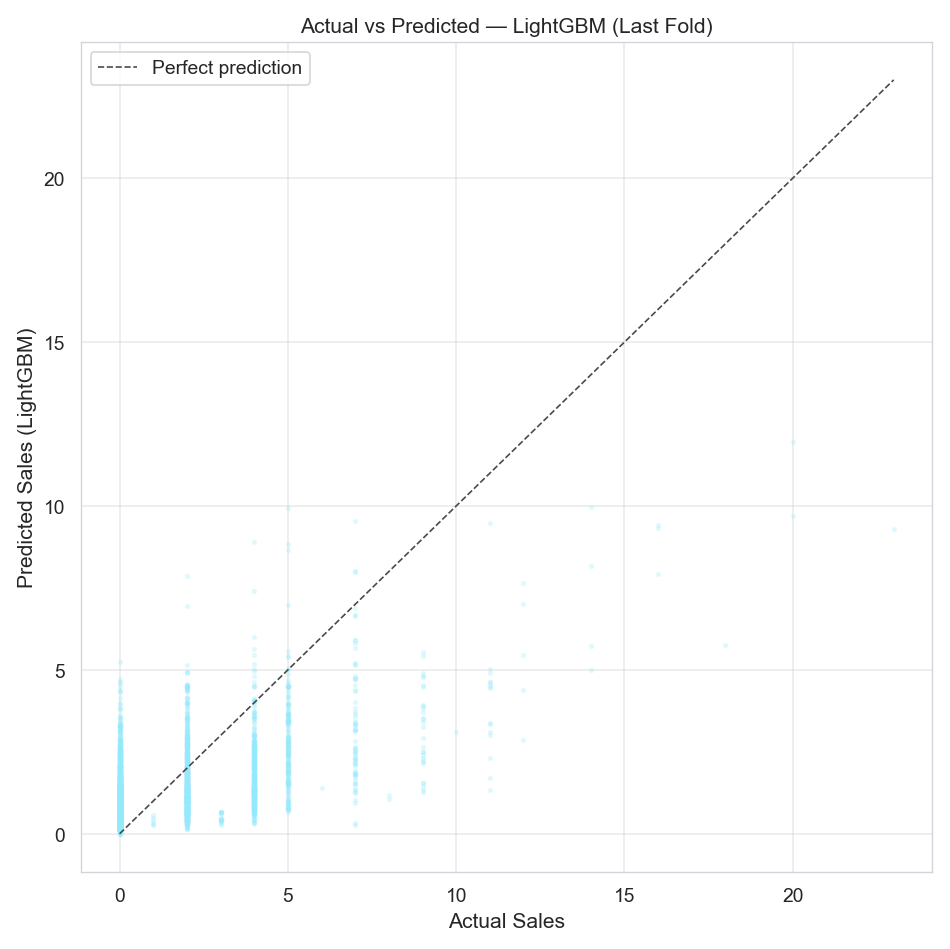
\includegraphics[width=0.85\textwidth]{figures/13_actual_vs_predicted_lgbm.png}
\caption{Actual vs.\ predicted sales for LightGBM on a sample of products. Points near the diagonal indicate accurate predictions; the cluster near the origin reflects the high proportion of zero-demand observations.}
\label{fig:actual_vs_predicted}
\end{figure}

\begin{figure}[H]
\centering
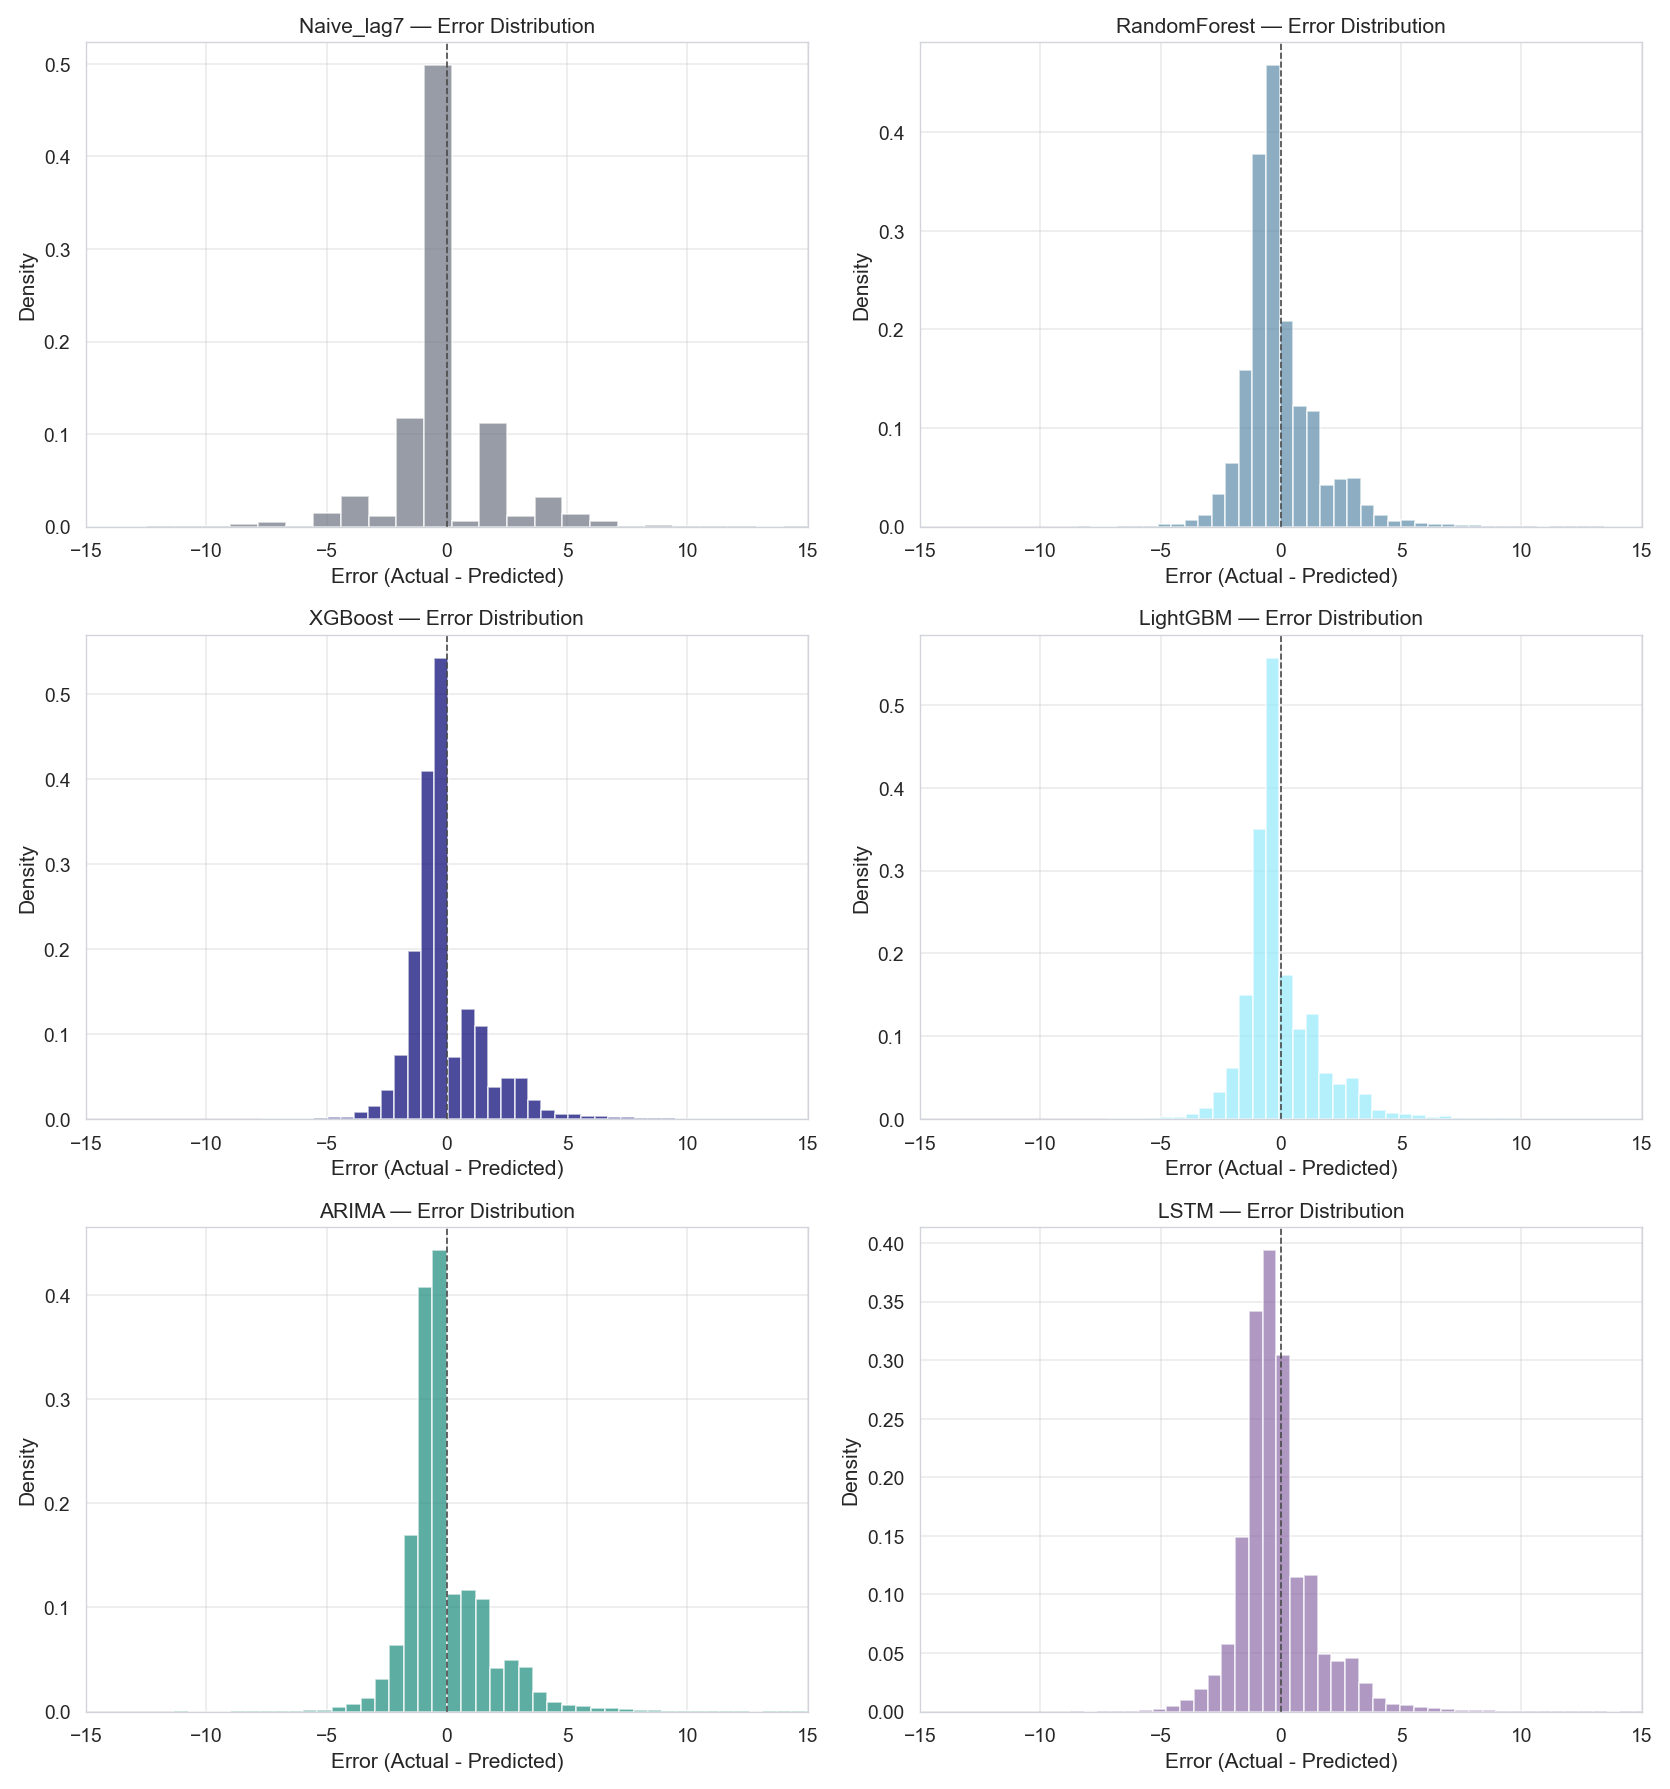
\includegraphics[width=0.85\textwidth]{figures/17_error_distributions.png}
\caption{Distribution of forecast errors by model. The ML models produce tighter, more symmetric error distributions compared to the naive baseline.}
\label{fig:error_distributions}
\end{figure}

\begin{figure}[H]
\centering
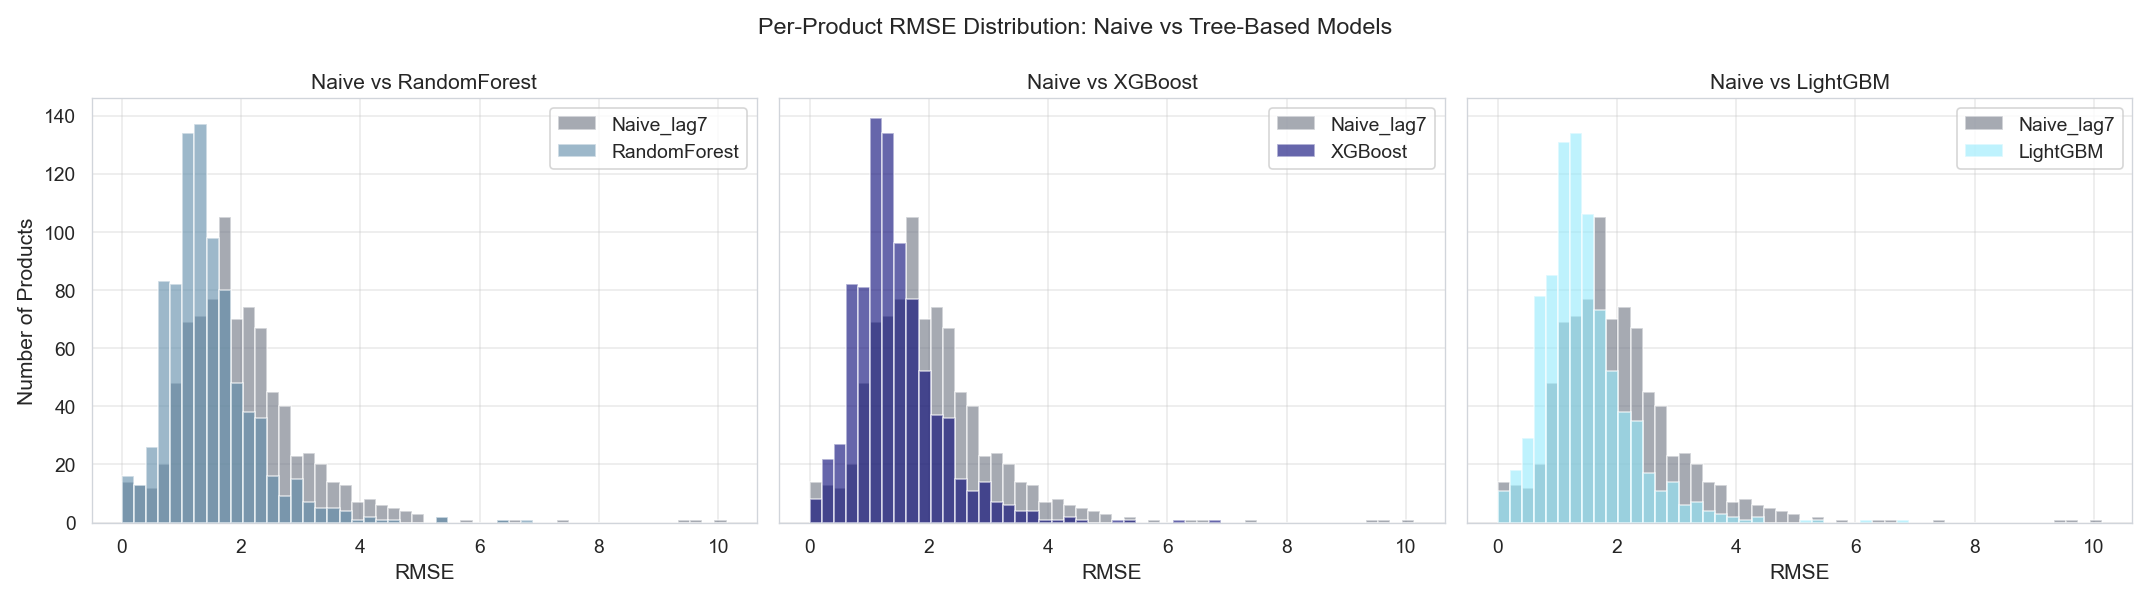
\includegraphics[width=0.85\textwidth]{figures/18_per_product_rmse_dist.png}
\caption{Distribution of per-product RMSE values. The ML models shift the distribution towards lower RMSE values compared to the naive baseline.}
\label{fig:per_product_rmse}
\end{figure}

\textbf{SHAP feature importance.} To understand the drivers of model predictions, SHAP (SHapley Additive exPlanations) analysis was performed on the LightGBM model. Table~\ref{tab:shap_top10} presents the ten most influential features:

\begin{table}[H]
\centering
\small
\caption{Top 10 features by mean absolute SHAP value (LightGBM).}
\label{tab:shap_top10}
\begin{tabular}{|r|l|r|}
\hline
\textbf{Rank} & \textbf{Feature} & \textbf{Mean $|$SHAP$|$} \\
\hline
1 & ewma\_28 & 0.524 \\
2 & bolHoliday & 0.295 \\
3 & roll\_mean\_28 & 0.150 \\
4 & day\_of\_week & 0.079 \\
5 & udsStock & 0.063 \\
6 & roll\_max\_28 & 0.046 \\
7 & lag\_28 & 0.025 \\
8 & bolOpen & 0.022 \\
9 & roll\_mean\_14 & 0.017 \\
10 & roll\_max\_14 & 0.016 \\
\hline
\end{tabular}
\end{table}

The 28-day EWMA emerges as the single most important predictor, followed by the holiday indicator and the 28-day rolling mean. This confirms that the model relies heavily on smoothed representations of recent demand history, with calendar effects providing secondary but significant predictive power. Notably, the longer-horizon features (28-day windows) dominate over shorter-horizon ones (7-day), suggesting that the model captures medium-term demand trends rather than relying solely on short-term momentum.

\begin{figure}[H]
\centering
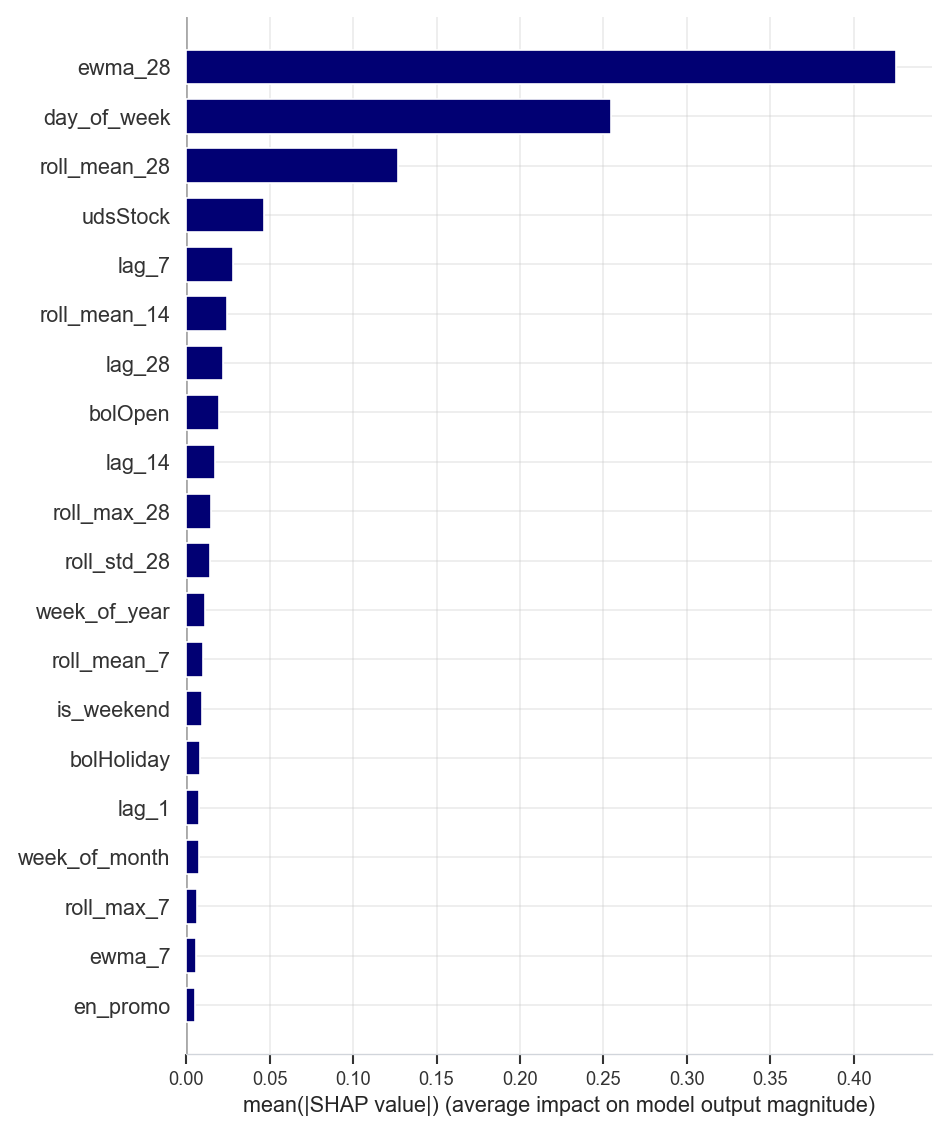
\includegraphics[width=0.85\textwidth]{figures/15_shap_bar.png}
\caption{SHAP feature importance (mean absolute SHAP values) for LightGBM. The 28-day EWMA dominates, followed by calendar and rolling statistics features.}
\label{fig:shap_bar}
\end{figure}

\begin{figure}[H]
\centering
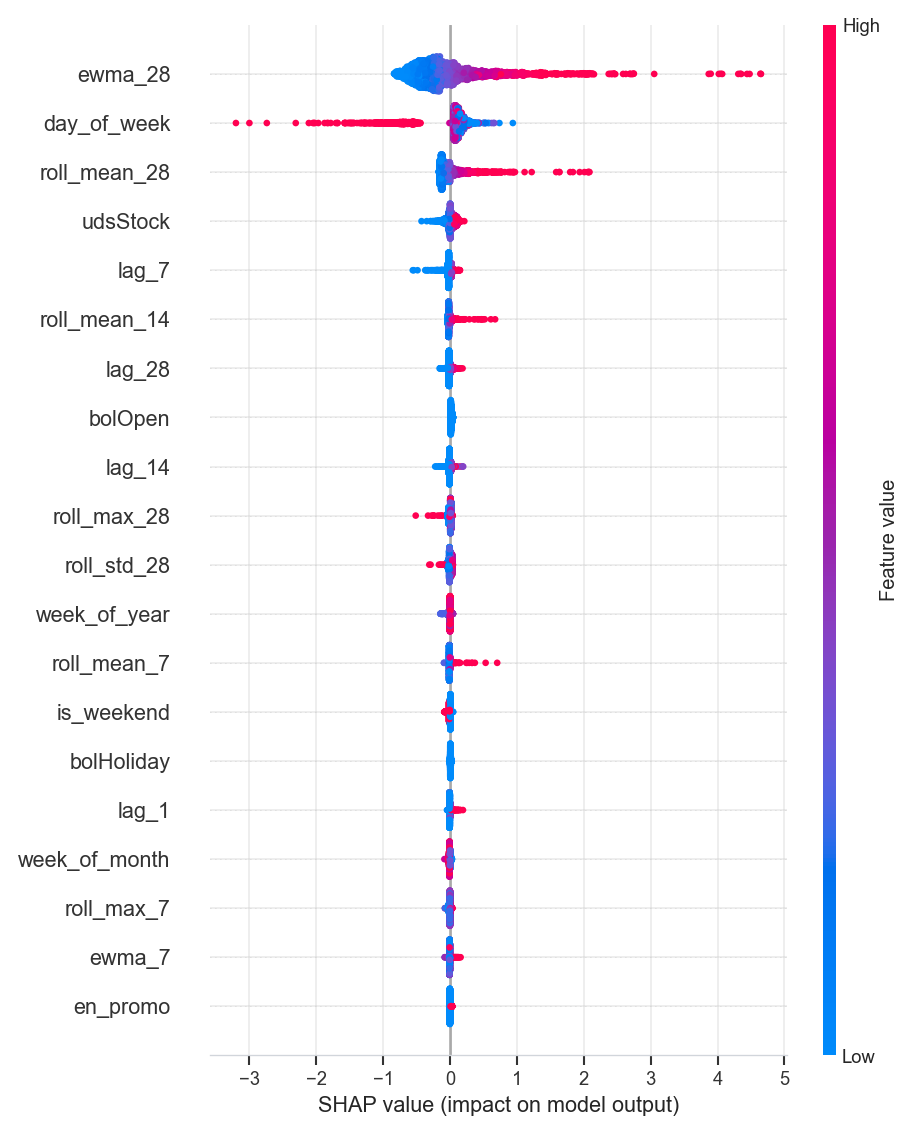
\includegraphics[width=0.85\textwidth]{figures/14_shap_summary.png}
\caption{SHAP summary plot showing the direction and magnitude of feature effects. Red indicates high feature values; blue indicates low values. High \texttt{ewma\_28} values push predictions upward, consistent with higher recent demand leading to higher forecasts.}
\label{fig:shap_summary}
\end{figure}

\subsection{Conclusions from Results}

The evaluation yields several key findings:

\begin{enumerate}
    \item The three tree-based machine learning models (XGBoost, LightGBM, Random Forest) achieve the best performance, with RMSE values within 1\% of each other. This suggests that the feature engineering, rather than the specific algorithm choice, is the primary driver of forecast quality among this model family.

    \item ARIMA and LSTM occupy an intermediate tier, both significantly outperforming the naive baseline (RMSE reductions of 28\% and 28\% respectively) but falling short of the tree-based models. ARIMA's per-product fitting captures local demand patterns effectively but cannot leverage cross-product information or engineered features. LSTM captures sequential dependencies but requires substantially more training data and computation to match tree-based performance.

    \item The improvement over the naive baseline is substantial across all ML approaches (28--30\% RMSE reduction), demonstrating the value of incorporating engineered features and systematic model training over simple heuristic forecasting.

    \item Promotional demand remains the most challenging segment, with RMSE approximately 38\% higher than non-promotional demand across all models. However, the ML models maintain their relative advantage over the baseline in both segments.

    \item SHAP analysis reveals that smoothed demand history (EWMA and rolling statistics) and calendar features are the most influential predictors, validating the feature engineering strategy adopted in this work.

    \item The forecast error standard deviation ($\sigma_e \approx 2.15$ for the best tree models, $\sigma_e \approx 2.22$ for ARIMA/LSTM, compared to $\sigma_e \approx 3.09$ for the naive baseline) translates directly into safety stock reductions, as quantified in the following section.
\end{enumerate}


\section{Impact of Algorithm Improvement}

\subsection{Impact on Processes}

The transition from a naive forecasting approach to machine learning models has implications beyond numerical accuracy improvements. From an operational perspective, the key process impacts are:

\textbf{Safety stock reduction.} Using the safety stock formulation from Equation~\ref{eq:safety_stock} with a 95\% service level ($z = 1.645$) and a protection period of 10 days (3 days lead time + 7 days review period), the total safety stock across all 894 products decreases from 11,953 units under the naive forecast to 8,276 units under LightGBM --- a reduction of 30.8\%. This means that the same service level can be maintained with significantly less inventory investment.

\textbf{Forecast error symmetry.} Analysis of error distributions shows that the ML models produce approximately symmetric errors centred near zero, whereas the naive baseline exhibits a slight positive bias (tendency to overforecast). Symmetric errors are preferable for inventory planning, as they indicate that the forecast is equally likely to overestimate or underestimate demand, allowing safety stock to function as intended.

\textbf{Sensitivity to service level.} Table~\ref{tab:sensitivity} presents the total safety stock requirements across different service levels:

\begin{table}[H]
\centering
\small
\caption{Total safety stock (units) by model and service level.}
\label{tab:sensitivity}
\begin{tabular}{|l|r|r|r|}
\hline
\textbf{Model} & \textbf{90\%} & \textbf{95\%} & \textbf{99\%} \\
\hline
LightGBM & 6,450 & 8,276 & 11,702 \\
XGBoost & 6,466 & 8,296 & 11,731 \\
Random Forest & 6,507 & 8,350 & 11,806 \\
Naive (lag-7) & 9,316 & 11,953 & 16,902 \\
\hline
\end{tabular}
\end{table}

The ML models consistently require approximately 30\% less safety stock than the naive baseline across all service levels, demonstrating that the improvement is robust and not dependent on a specific service level assumption.

\begin{figure}[H]
\centering
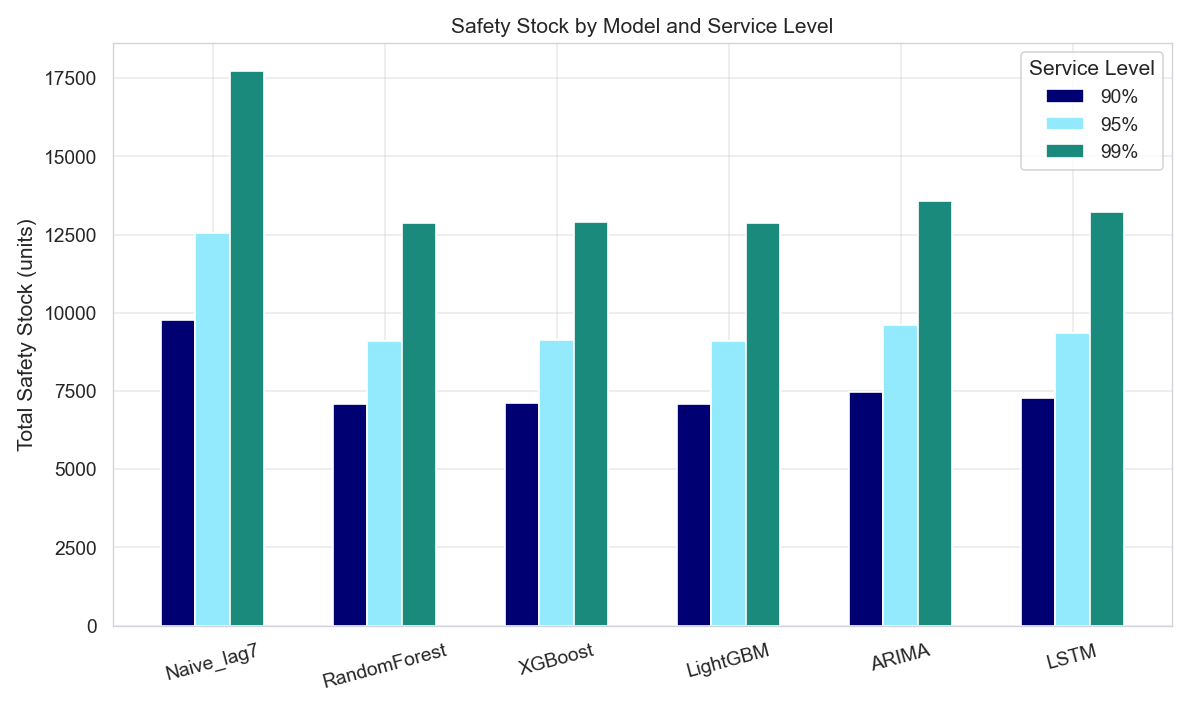
\includegraphics[width=0.85\textwidth]{figures/21_safety_stock_by_service_level.png}
\caption{Total safety stock requirements by model and service level. The ML models maintain a consistent ~30\% advantage over the naive baseline across all service levels.}
\label{fig:safety_stock_service_level}
\end{figure}

\subsection{Economic Impact}

The economic impact analysis combines two cost components: the newsvendor cost (direct cost of forecast errors) and the safety stock holding cost.

\textbf{Newsvendor cost analysis.} Following the total cost formulation from Equation~\ref{eq:total_cost}, the asymmetric costs of overforecasting and underforecasting were computed using cost parameters of $C_o = \text{\euro}0.10$ per unit per day (overage/holding) and $C_u = \text{\euro}0.50$ per unit per day (underage/lost sale), yielding a critical ratio of 0.83. These values reflect a typical retail/industrial setting where stockout costs substantially exceed holding costs.

Table~\ref{tab:newsvendor} presents the newsvendor cost results:

\begin{table}[H]
\centering
\small
\caption{Newsvendor cost analysis (30-day test period, annualised).}
\label{tab:newsvendor}
\begin{tabular}{|l|r|r|r|r|}
\hline
\textbf{Model} & \textbf{Overage (€)} & \textbf{Underage (€)} & \textbf{Total (€)} & \textbf{Annual est. (€)} \\
\hline
Naive (lag-7) & 2,227 & 11,138 & 13,365 & 162,603 \\
Random Forest & 1,830 & 9,538 & 11,367 & 138,304 \\
LightGBM & 1,786 & 9,489 & 11,275 & 137,182 \\
XGBoost & 1,785 & 9,392 & 11,176 & 135,979 \\
\hline
\end{tabular}
\end{table}

XGBoost achieves the lowest newsvendor cost, saving approximately \euro26,600 annually (16.4\%) compared to the naive baseline. Underage costs dominate in all models, consistent with the asymmetric cost structure where stockouts are five times more expensive than excess inventory.

\textbf{Combined cost analysis.} Table~\ref{tab:combined_cost} presents the total annual cost combining newsvendor costs with safety stock holding costs at the 95\% service level:

\begin{table}[H]
\centering
\small
\caption{Combined annual cost: newsvendor + safety stock holding (95\% service level).}
\label{tab:combined_cost}
\begin{tabular}{|l|r|r|r|}
\hline
\textbf{Model} & \textbf{Newsvendor (€/yr)} & \textbf{SS Holding (€/yr)} & \textbf{Total (€/yr)} \\
\hline
Naive (lag-7) & 162,603 & 436,294 & 598,896 \\
Random Forest & 138,304 & 304,763 & 443,067 \\
LightGBM & 137,182 & 302,083 & 439,265 \\
XGBoost & 135,979 & 302,816 & 438,796 \\
\hline
\end{tabular}
\end{table}

The ML models achieve total annual cost savings of approximately \euro160,000 (26.7\%) compared to the naive baseline. XGBoost and LightGBM perform nearly identically in economic terms, with XGBoost holding a marginal advantage of \euro469 annually.

\begin{figure}[H]
\centering
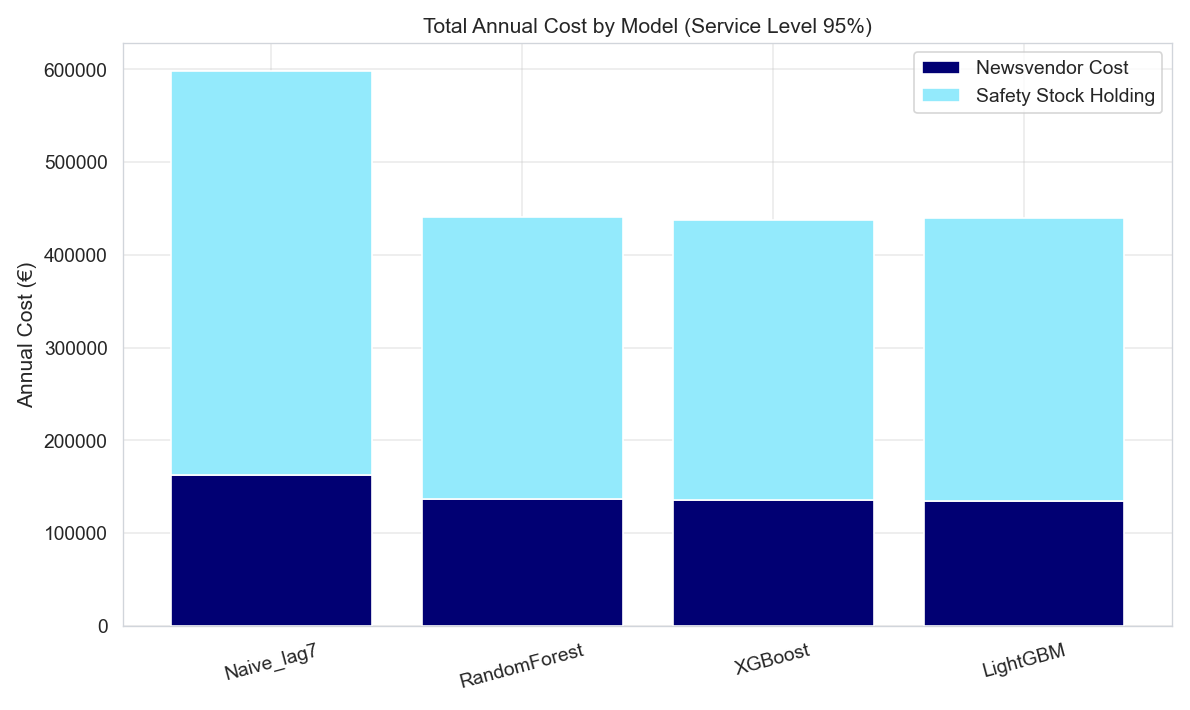
\includegraphics[width=0.85\textwidth]{figures/22_combined_annual_cost.png}
\caption{Combined annual inventory cost (newsvendor + safety stock holding) by model. The ML models reduce total costs by approximately 26.7\% compared to the naive baseline.}
\label{fig:combined_annual_cost}
\end{figure}

These results demonstrate that the forecast accuracy improvements documented in Section~3.6 translate into meaningful economic benefits. The 28\% reduction in RMSE corresponds to a 26.7\% reduction in total inventory-related costs, confirming the theoretical relationship between forecast error and inventory costs established in Chapter~2 (Equations~\ref{eq:ss_cost} and \ref{eq:total_cost}).

It is important to note that the cost parameters used in this analysis ($C_o$ and $C_u$) are illustrative values chosen to reflect typical industrial cost structures. The relative ranking of models and the percentage savings are robust to reasonable variations in these parameters, as the underlying driver is the reduction in forecast error rather than the specific cost assumptions. A sensitivity analysis across service levels (Table~\ref{tab:sensitivity}) confirms that the ML advantage is maintained regardless of the risk tolerance adopted by the organisation.
 in TFM_onamas.tex

This chapter presents the complete design and implementation of the demand forecasting system, following the CRISP-DM methodology introduced in Chapter~1. The work progresses from data acquisition and exploration through preprocessing, feature engineering, model development, evaluation, and finally the economic impact analysis that connects forecast accuracy to inventory cost savings.

\section{Data Origin}

\subsection{Data Acquisition}

The dataset used in this project was provided by the thesis supervisor and corresponds to real historical data from a company operating in the automotive sector. The data covers daily demand records for a portfolio of products, along with supplementary information on calendar events, promotional campaigns, and stock levels. All data was received in a single Microsoft Excel file (\texttt{Datos.xlsx}) containing four sheets, each representing a distinct dimension of the business context.

No personally identifiable information is present in the dataset, and all product references are anonymised using numerical identifiers, ensuring compliance with data privacy requirements as discussed in Section~\ref{s:etic}.

\subsection{Data Description}

The dataset comprises four tables, summarised in Table~\ref{tab:data_sheets}:

\begin{table}[H]
\centering
\small
\caption{Structure of the source dataset (\texttt{Datos.xlsx}).}
\label{tab:data_sheets}
\begin{tabular}{|l|l|r|p{5.5cm}|}
\hline
\textbf{Sheet} & \textbf{Key columns} & \textbf{Rows} & \textbf{Description} \\
\hline
Ventas (Sales) & producto, fecha, udsVenta & 654,588 & Daily unit sales per product \\
\hline
Calendario & fecha, bolOpen, bolHoliday & 732 & Calendar flags: business day and holiday indicators \\
\hline
Promociones & producto, fechaInicio, fechaFin & 1,894 & Promotional campaign periods per product \\
\hline
Stock & producto, fecha, udsStock & 654,588 & Daily stock levels per product \\
\hline
\end{tabular}
\end{table}

The sales sheet constitutes the core of the dataset, containing 654,588 daily observations across 894 unique products over a period of 732 days, spanning from November 2022 to November 2024. Each record represents the number of units sold for a specific product on a specific date.

The calendar sheet provides 732 daily records with two binary indicators: \texttt{bolOpen} (whether the business was open) and \texttt{bolHoliday} (whether the date was a public holiday). The promotions sheet contains 1,894 records defining promotional campaign windows through start and end dates for each product. The stock sheet mirrors the sales structure, recording the closing stock level for each product-date combination.

\subsection{Data Loading}

All four sheets were loaded into memory using the \texttt{pandas} library with the \texttt{openpyxl} engine. The sales and stock tables were merged on the shared keys \texttt{(producto, fecha)}, and the calendar information was joined on \texttt{fecha}. Promotional periods were transformed from date ranges into a binary indicator (\texttt{en\_promo}) at the product-date level, marking each observation as promotional or non-promotional based on whether the date fell within any active campaign for that product.

After merging, the resulting dataset contained 654,588 rows and served as the foundation for all subsequent analysis. The merged dataset was persisted in Apache Parquet format for efficient reloading in downstream scripts.


\section{Data Exploration}

\subsection{Data Summary}

An initial statistical summary of the target variable (\texttt{udsVenta}, units sold) revealed a highly skewed distribution. The mean daily sales per product were 1.42 units, with a median of zero and a standard deviation of 3.56. The maximum observed value was 99 units. This distribution reflects the nature of automotive parts demand, where the majority of product-day combinations register zero sales, punctuated by occasional larger orders.

Table~\ref{tab:sales_stats} presents the key descriptive statistics:

\begin{table}[H]
\centering
\small
\caption{Descriptive statistics of daily unit sales (\texttt{udsVenta}).}
\label{tab:sales_stats}
\begin{tabular}{|l|r|}
\hline
\textbf{Statistic} & \textbf{Value} \\
\hline
Count & 654,588 \\
Mean & 1.42 \\
Std. deviation & 3.56 \\
Median (50\%) & 0.00 \\
75th percentile & 1.00 \\
95th percentile & 7.00 \\
Maximum & 99 \\
Zero-sales proportion & 64.5\% \\
\hline
\end{tabular}
\end{table}

The high proportion of zero-sales observations (64.5\%) is a defining characteristic of this dataset and has important implications for model selection and evaluation, as discussed in subsequent sections.

\begin{figure}[H]
\centering
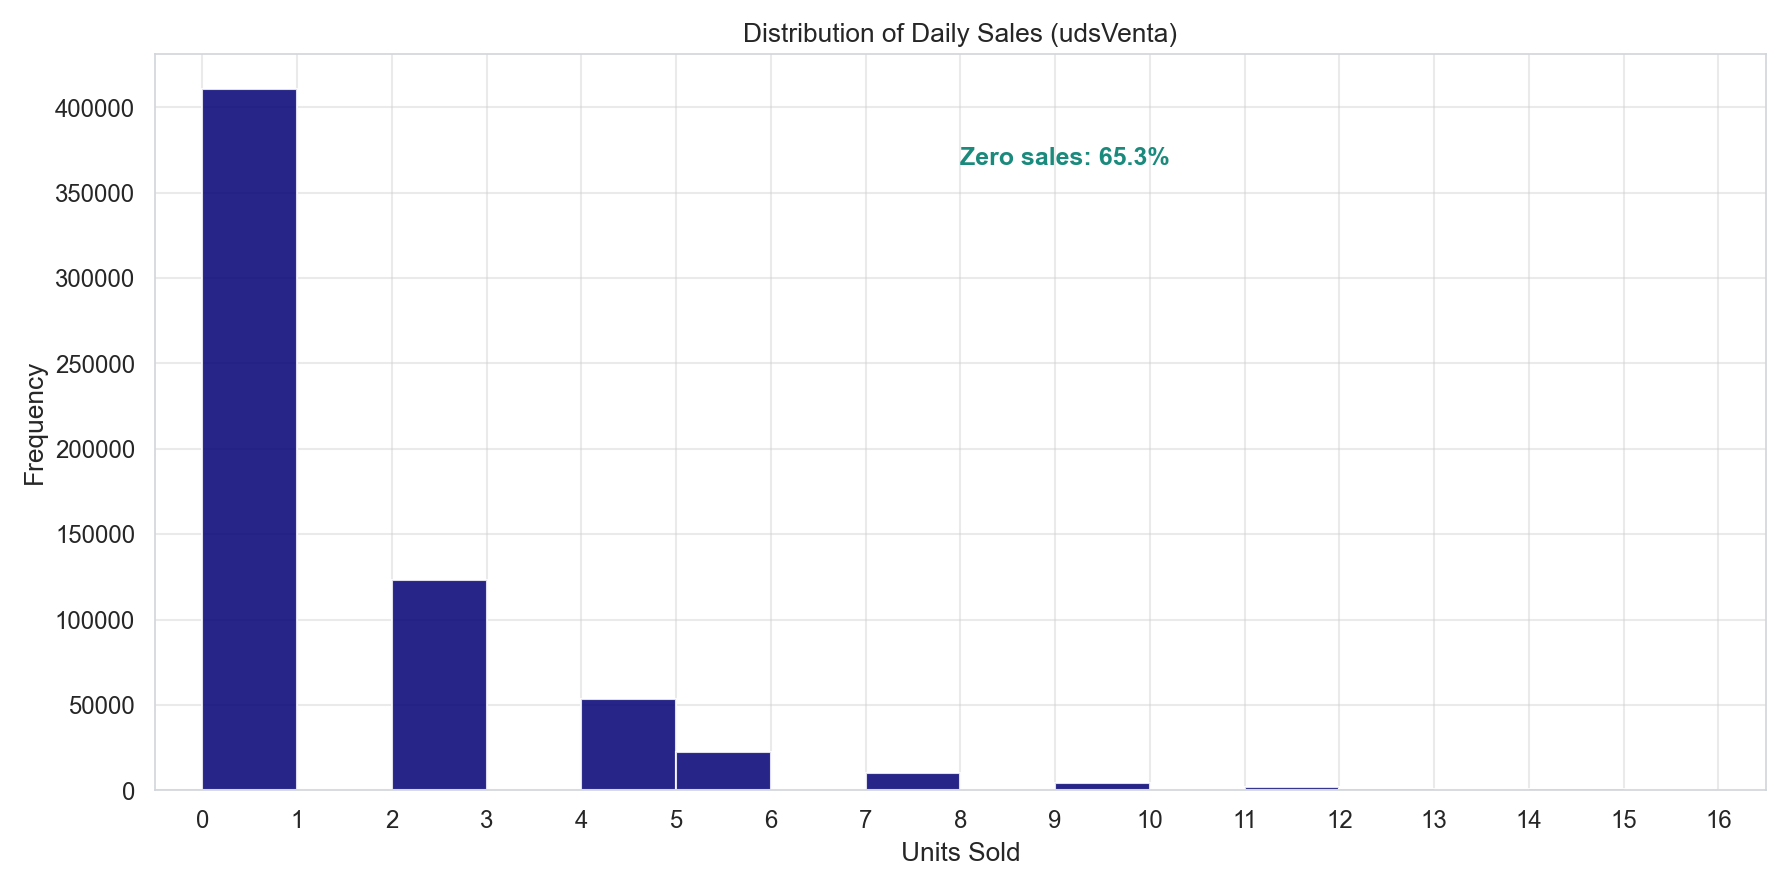
\includegraphics[width=0.85\textwidth]{figures/01_sales_distribution.png}
\caption{Distribution of daily unit sales (\texttt{udsVenta}). The histogram confirms the extreme right skew, with the majority of observations at zero.}
\label{fig:sales_distribution}
\end{figure}

\subsection{Statistical Analysis}

The exploratory analysis examined demand patterns across several dimensions:

\textbf{Day-of-week patterns.} Sales exhibit a clear weekly cycle, with the highest volumes on weekdays (Monday through Friday) and a sharp decline on Saturdays. Sunday sales are near zero, consistent with the business being closed on Sundays as indicated by the \texttt{bolOpen} calendar flag. This weekly seasonality motivates the inclusion of day-of-week features and the use of a lag-7 naive baseline (same weekday, previous week) as the primary benchmark.

\begin{figure}[H]
\centering
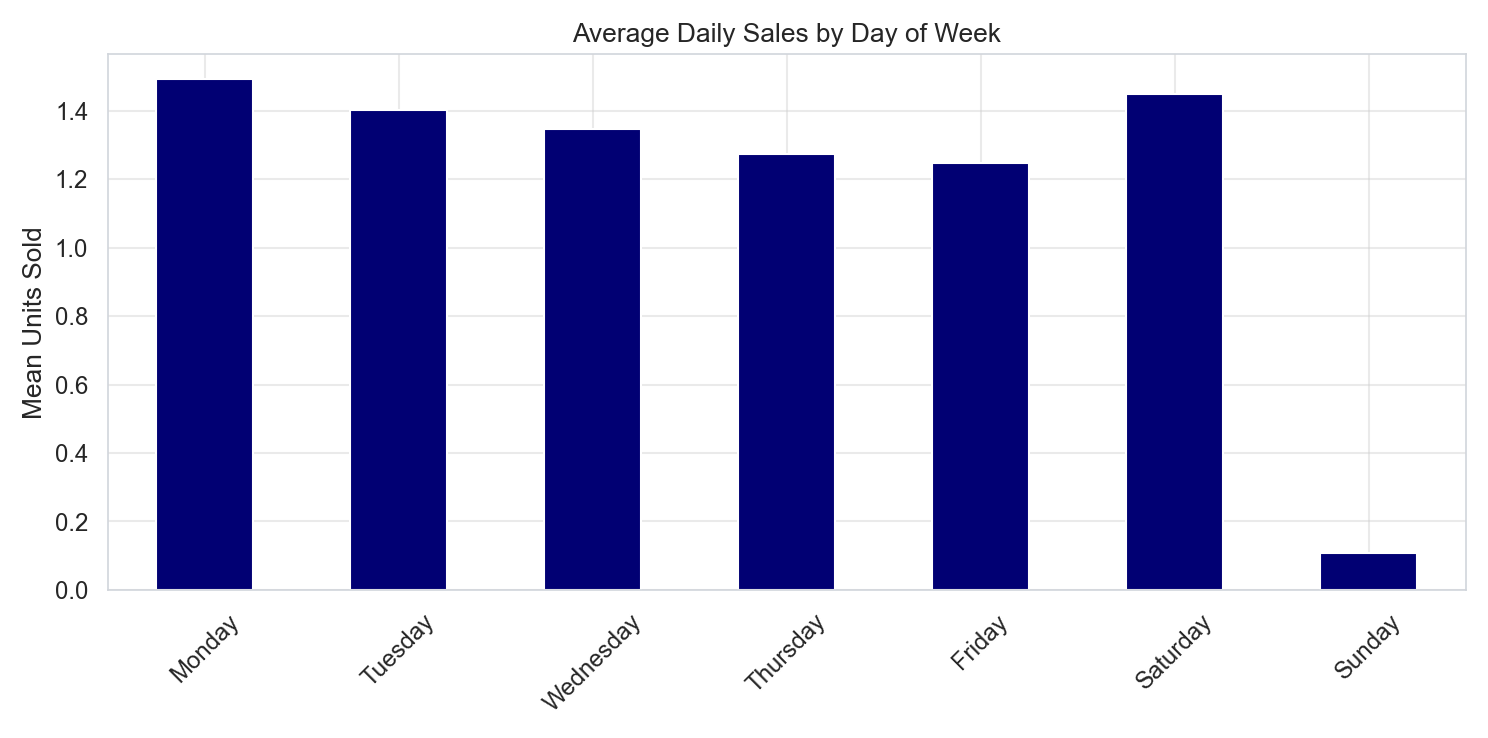
\includegraphics[width=0.85\textwidth]{figures/02_sales_by_day_of_week.png}
\caption{Average daily sales by day of the week. The weekly cycle is clearly visible, with near-zero sales on Sundays.}
\label{fig:sales_by_dow}
\end{figure}

\textbf{Monthly and seasonal patterns.} Monthly aggregated sales show moderate variation across the year, without a single dominant seasonal peak. However, certain months consistently show higher activity, suggesting that calendar-based features (month, week of year) may contribute predictive value.

\textbf{Promotional effects.} Comparing sales during promotional and non-promotional periods revealed that mean sales during promotions (1.83 units) were slightly higher than during non-promotional periods (1.38 units). However, the difference is modest, and the promotional flag alone does not capture the full complexity of promotional demand dynamics, which motivated the engineering of additional promotional features described in Section~3.4.

\begin{figure}[H]
\centering
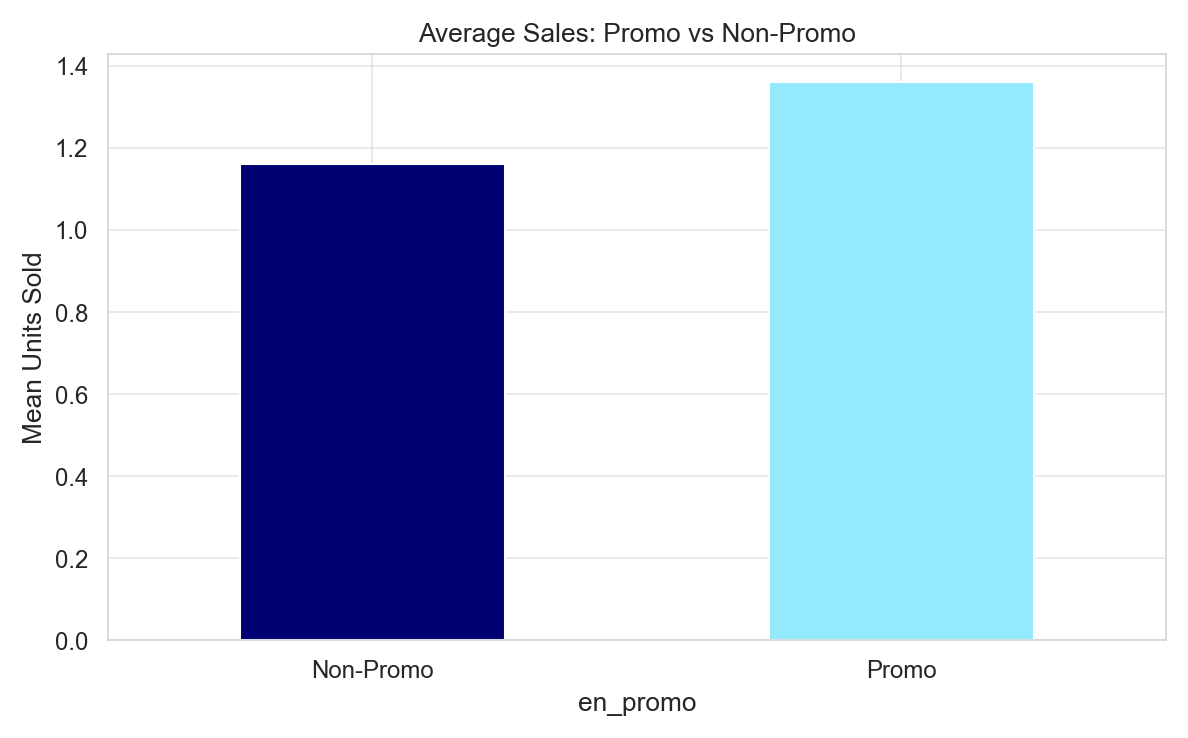
\includegraphics[width=0.85\textwidth]{figures/05_promo_vs_nonpromo.png}
\caption{Comparison of sales distributions during promotional and non-promotional periods.}
\label{fig:promo_vs_nonpromo}
\end{figure}

\textbf{Autocorrelation structure.} Autocorrelation analysis on a sample of products confirmed significant positive autocorrelation at lags 1, 7, 14, and 28, with the strongest signal at lag 7 (weekly periodicity). This finding directly supports the creation of lag features at these intervals and validates the choice of lag-7 as the naive baseline.

\begin{figure}[H]
\centering
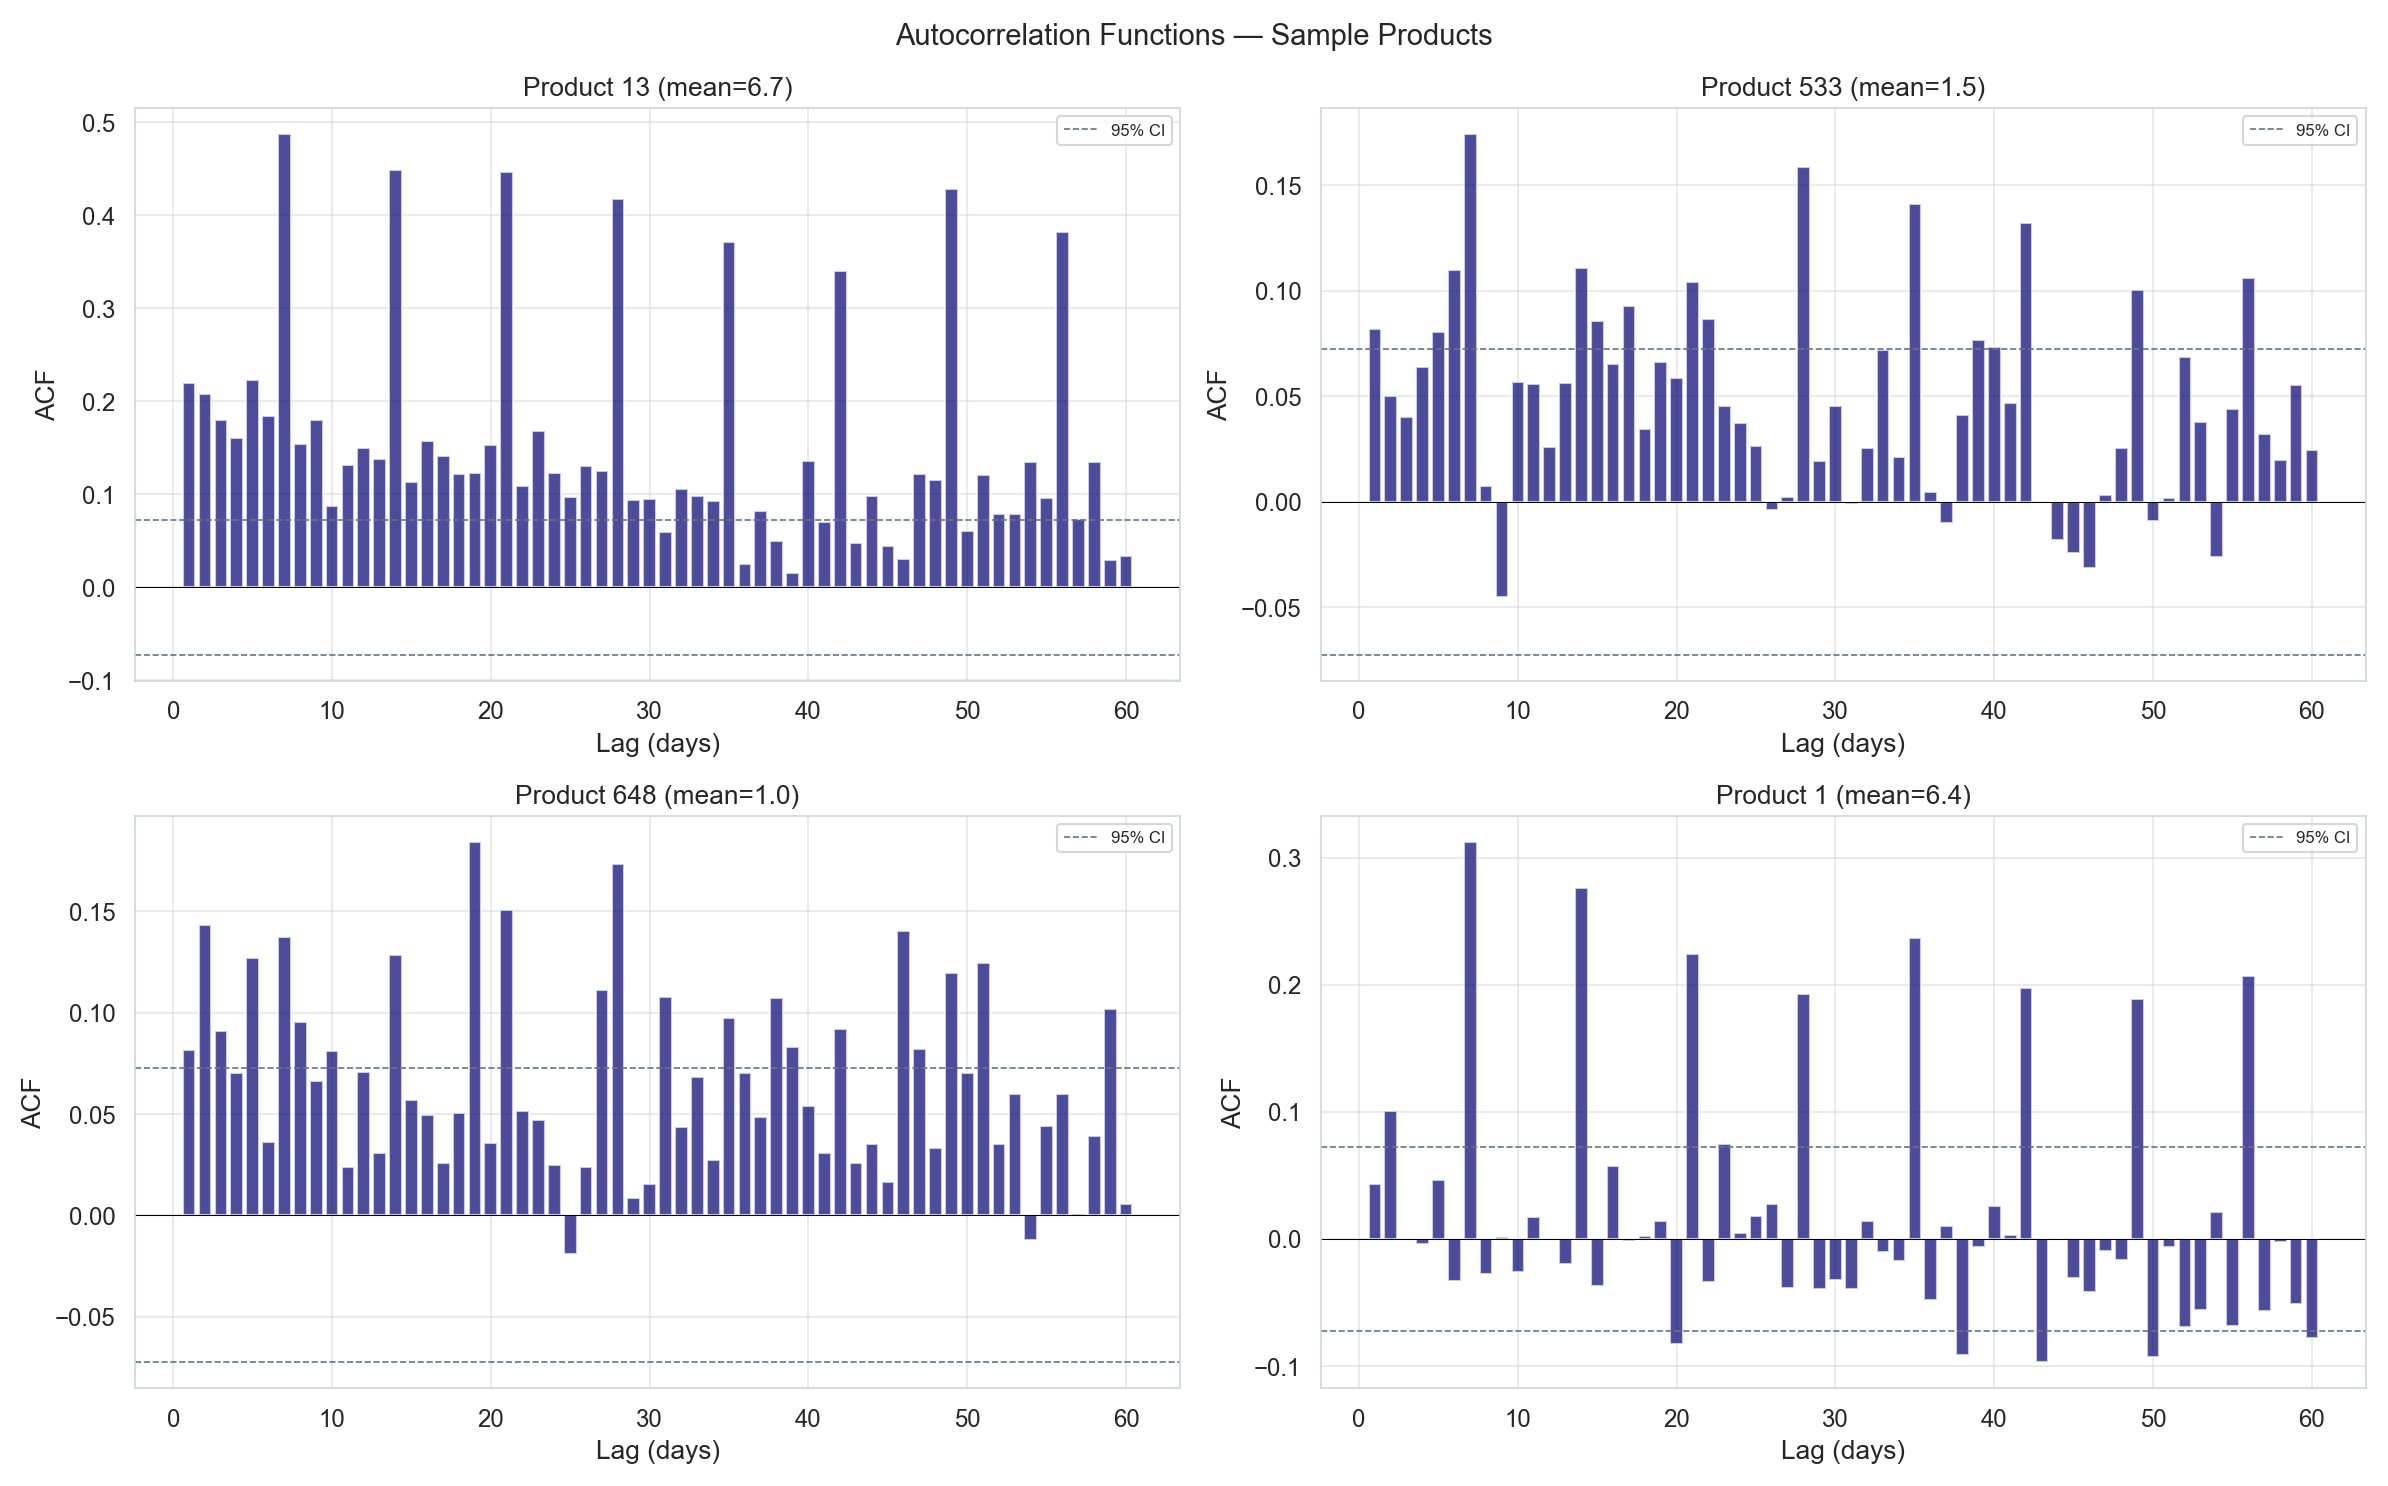
\includegraphics[width=0.85\textwidth]{figures/08_autocorrelation_sample.png}
\caption{Autocorrelation function (ACF) for a sample of products, showing significant positive autocorrelation at weekly intervals.}
\label{fig:autocorrelation}
\end{figure}

\subsection{Data Quality Analysis}

The data quality assessment identified the following issues:

\textbf{Missing values.} No explicit missing values were found in any of the four source tables. However, implicit gaps exist where lag features cannot be computed for the earliest dates in each product's history (addressed during feature engineering).

\textbf{Negative values.} No negative sales or stock values were present in this dataset.

\textbf{Stock breaks.} A stock break is defined as a day where both sales and stock are zero, potentially indicating that demand existed but could not be fulfilled due to inventory unavailability. Approximately 3.9\% of observations met this criterion. These were treated during data cleaning by imputing the product's historical mean sales for the corresponding weekday.

\textbf{Outliers.} Outlier detection was performed using a threshold of 1.75 times the interquartile range (IQR) per product. This identified approximately 11,400 observations (1.75\% of the dataset) as outliers, which were capped at the upper threshold value. The IQR-based approach was preferred over a fixed standard deviation threshold to account for the varying demand scales across products.


\section{Data Preparation}

\subsection{Data Cleaning}

The data cleaning process addressed the two quality issues identified during exploration:

\begin{enumerate}
    \item \textbf{Stock break imputation:} For observations where both \texttt{udsVenta} and \texttt{udsStock} were zero, the sales value was replaced with the mean sales for that product on the same weekday, computed over the preceding 30 days. This approach assumes that zero sales on a day with zero stock reflects a supply-side constraint rather than genuine zero demand, and uses a localised historical average to provide a reasonable demand estimate.

    \item \textbf{Outlier capping:} Values exceeding 1.75 $\times$ IQR above the 75th percentile for each product were capped at the threshold value. This preserves the general distribution shape while limiting the influence of extreme observations on model training. A total of 11,400 values (1.75\% of the dataset) were capped.
\end{enumerate}

After cleaning, the dataset retained its original 654,588 rows with no records removed, ensuring that the temporal continuity required for lag feature computation was preserved.

\subsection{Data Transformation}

The date column (\texttt{fecha}) was parsed into a \texttt{datetime} type, and the dataset was sorted by product and date to ensure correct temporal ordering for all subsequent operations. The promotional periods from the source data were transformed from date-range format into a daily binary indicator (\texttt{en\_promo}), assigned at the product-date level.

No logarithmic or power transformations were applied to the target variable. While such transformations can stabilise variance in skewed distributions, the tree-based models used in this work (Random Forest, XGBoost, LightGBM) are inherently robust to non-normal distributions and do not require target transformation for effective learning.

\subsection{Data Scaling}

Feature scaling (standardisation or normalisation) was not applied for the tree-based models, as decision tree ensembles are invariant to monotonic transformations of input features. The split-based learning mechanism of these algorithms operates on feature rankings rather than absolute values, making scaling unnecessary.

For the LSTM model, min-max normalisation was applied to all input features to facilitate gradient-based optimisation. Each feature was scaled to the $[0, 1]$ range using the training set statistics, and the same transformation was applied to the validation and test sets to prevent information leakage. Predictions were inverse-transformed back to the original scale before computing evaluation metrics.

\section{Feature Engineering}

Feature engineering is a central component of this work. A comprehensive set of 36 engineered features was designed to capture temporal dependencies, demand dynamics, and promotional effects. The features are organised into five categories, summarised in Table~\ref{tab:features}.

\begin{table}[H]
\centering
\small
\caption{Engineered features by category.}
\label{tab:features}
\begin{tabular}{|l|p{7cm}|r|}
\hline
\textbf{Category} & \textbf{Features} & \textbf{Count} \\
\hline
Original variables & udsStock, bolOpen, bolHoliday, en\_promo & 4 \\
\hline
Calendar features & year, month, day\_of\_week, week\_of\_year, week\_of\_month, is\_weekend, is\_month\_start, is\_month\_end & 8 \\
\hline
Lag features & lag\_1, lag\_7, lag\_14, lag\_28 & 4 \\
\hline
Rolling statistics & roll\_mean/std/min/max at 7, 14, and 28-day windows; ewma\_7, ewma\_28 & 14 \\
\hline
Promotional features & days\_since\_promo\_end, post\_promo\_7d, promo\_x\_lag7 & 3 \\
\hline
Product-level statistics & prod\_mean\_sales, prod\_std\_sales, prod\_median\_sales & 3 \\
\hline
\multicolumn{2}{|r|}{\textbf{Total}} & \textbf{36} \\
\hline
\end{tabular}
\end{table}

\textbf{Lag features} capture the autoregressive structure identified during exploration. The lag-7 feature (same weekday, previous week) serves dual purpose: it is used directly as the naive baseline forecast and as an input feature for the machine learning models. Lags at 1, 14, and 28 days capture short-term momentum, biweekly patterns, and monthly cycles respectively.

\textbf{Rolling statistics} provide smoothed representations of recent demand behaviour. For each window size (7, 14, and 28 days), the mean, standard deviation, minimum, and maximum of past sales are computed. Additionally, exponentially weighted moving averages (EWMA) with spans of 7 and 28 days provide adaptive smoothing that gives greater weight to more recent observations.

\textbf{Promotional features} go beyond the binary indicator to capture the temporal dynamics of promotions. The \texttt{days\_since\_promo\_end} feature tracks the recency of the last promotional period, \texttt{post\_promo\_7d} flags the week immediately following a promotion (to capture post-promotional demand depression), and \texttt{promo\_x\_lag7} is an interaction term between the promotional flag and the lag-7 sales value.

All lag and rolling features were computed strictly using past data to prevent information leakage. Observations where lag features could not be computed (the first 28 days of each product's history) were dropped, reducing the dataset from 654,588 to 629,370 rows. The final feature matrix was saved in Parquet format for use in the modelling phase.

\begin{figure}[H]
\centering
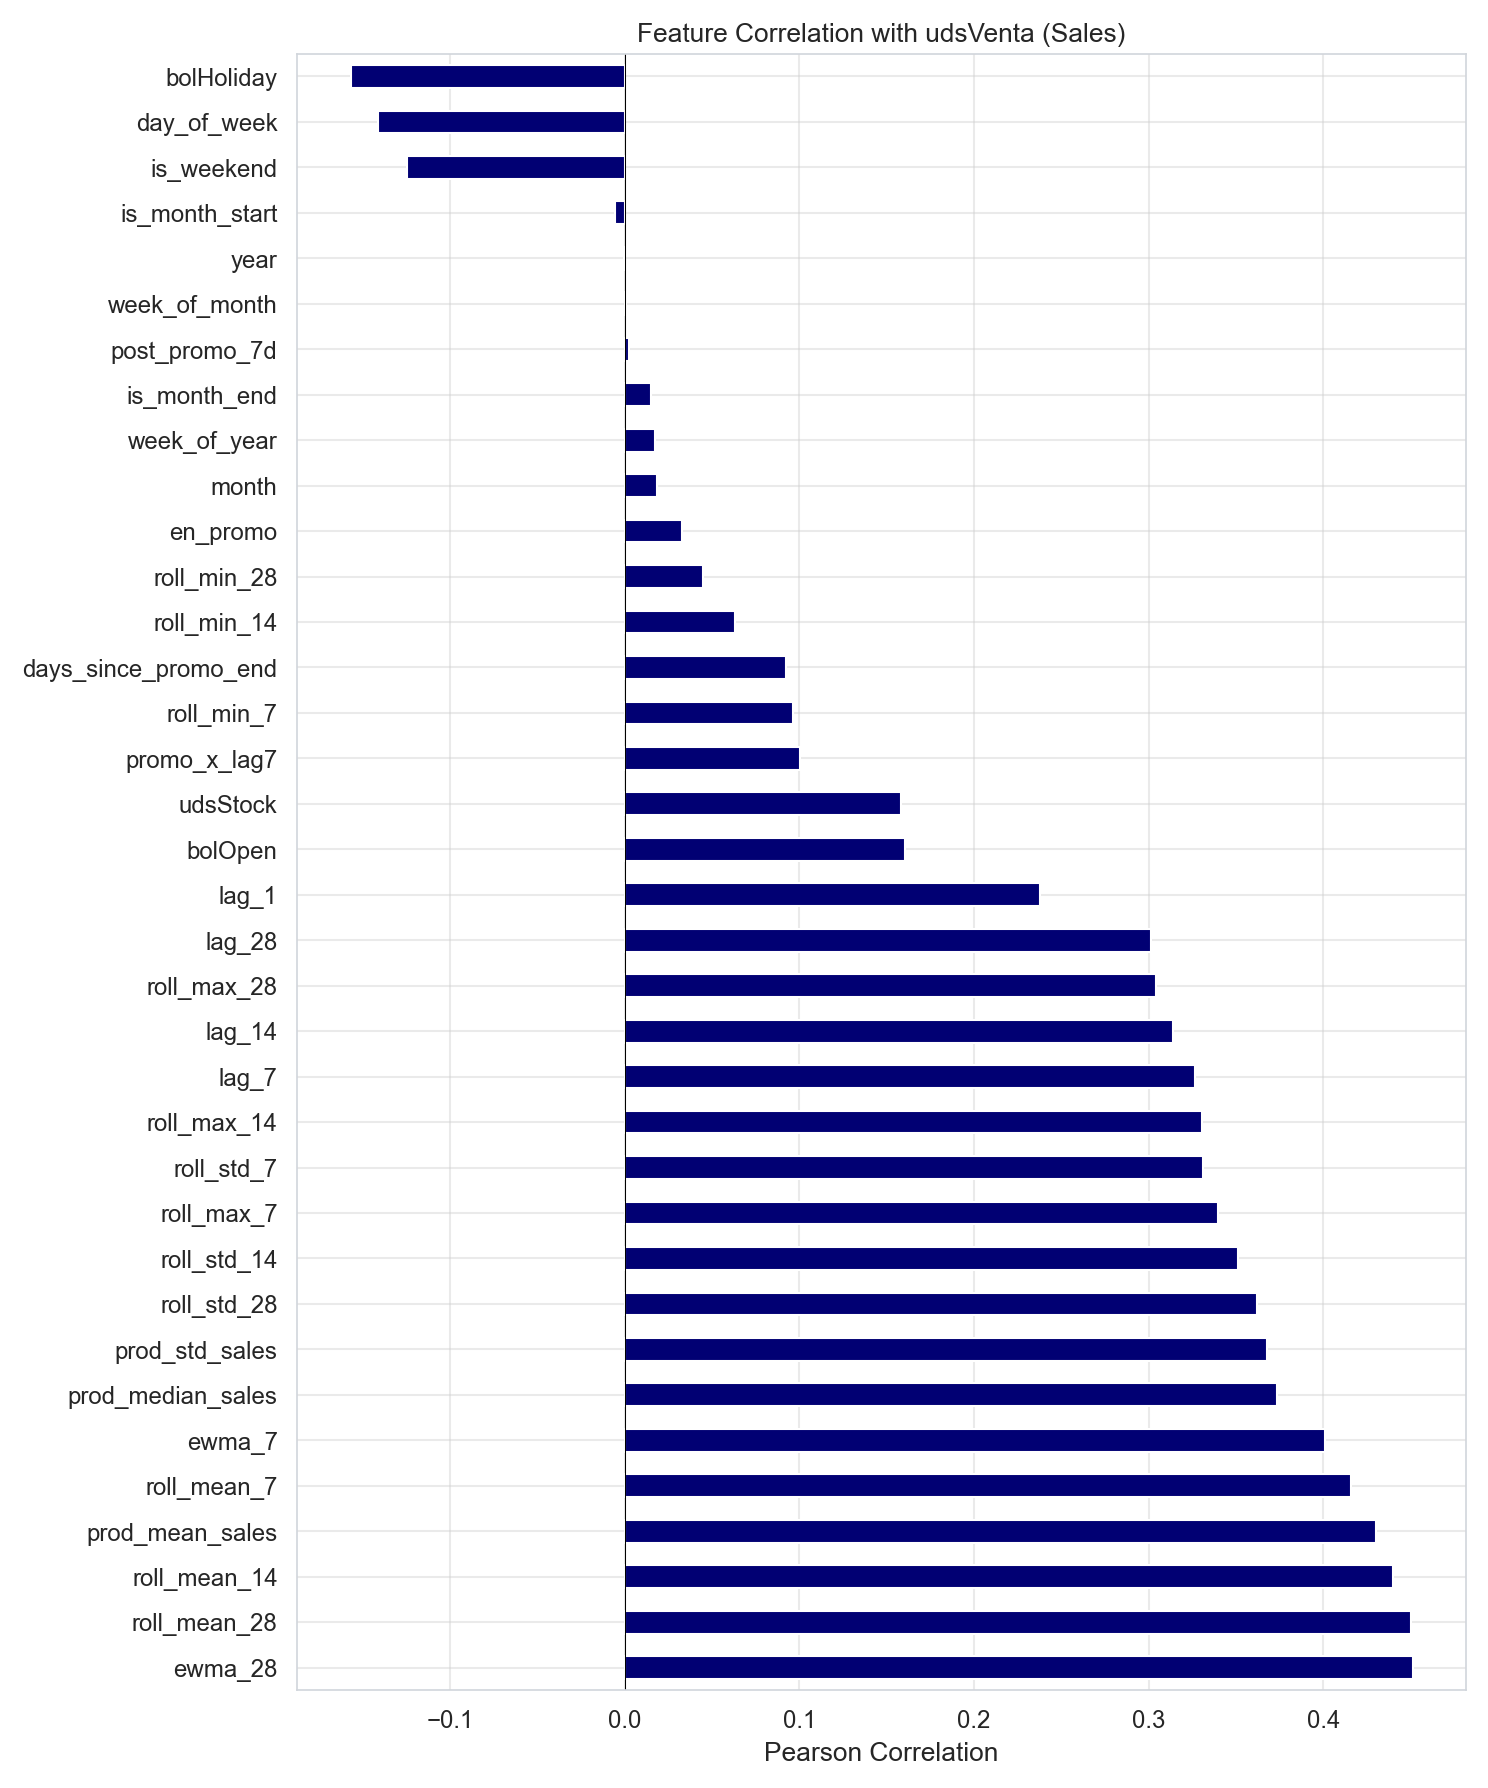
\includegraphics[width=0.95\textwidth]{figures/10_feature_correlations.png}
\caption{Correlation matrix of the engineered features. Strong correlations are visible among rolling statistics at different window sizes, confirming the presence of redundant but complementary temporal signals.}
\label{fig:feature_correlations}
\end{figure}


\section{Modelling}

\subsection{Model Selection}

Four forecasting approaches were implemented, spanning a naive baseline and three gradient boosting / ensemble methods:

\begin{enumerate}
    \item \textbf{Naive baseline (lag-7):} The simplest possible forecast, predicting that demand on any given day equals the demand observed on the same weekday of the previous week. This baseline exploits the strong weekly autocorrelation identified during exploration and provides a meaningful benchmark against which machine learning models must demonstrate improvement.

    \item \textbf{ARIMA (Seasonal):} A classical time series approach fitted per product using the \texttt{auto\_arima} implementation from the \texttt{pmdarima} library. Each product's demand series was modelled with seasonal ARIMA (SARIMA) with weekly periodicity ($m=7$), automatically selecting the optimal $(p,d,q)(P,D,Q)_7$ orders via stepwise search. ARIMA serves as the classical statistical baseline, representing the best that traditional time series methods can achieve without engineered features.

    \item \textbf{Random Forest:} An ensemble of decision trees trained on bootstrap samples with random feature subsets \citep{hyndman2021forecasting}. Random Forest provides robust predictions with built-in protection against overfitting through bagging and feature randomisation.

    \item \textbf{XGBoost:} A gradient boosting framework that builds trees sequentially, with each tree correcting the errors of its predecessors. XGBoost incorporates L1 and L2 regularisation, column subsampling, and efficient handling of sparse data, making it well-suited to the high proportion of zero-demand observations in this dataset.

    \item \textbf{LightGBM:} A gradient boosting implementation that uses histogram-based splitting and leaf-wise tree growth, offering faster training times than XGBoost while maintaining competitive accuracy. LightGBM was among the dominant algorithms in the M5 forecasting competition \citep{makridakis2021m5findings}.

    \item \textbf{LSTM (Long Short-Term Memory):} A recurrent neural network architecture designed to capture long-range temporal dependencies in sequential data \citep{hochreiter1997lstm}. Unlike tree-based methods, which rely on engineered lag features, LSTM processes input data as ordered sequences, with its internal gating mechanism allowing it to selectively retain or discard information from previous time steps. The model was implemented in PyTorch with a single LSTM layer (32 hidden units), trained on standardised features using 14-day input sequences.
\end{enumerate}

All tree-based models were trained on the full set of 33 input features (the 36 engineered features minus the 3 product-level statistics used only for reference). ARIMA was fitted per product on the raw sales series without engineered features, as is standard for classical time series methods. The LSTM model received the same 33 features as the tree models, but processed them as ordered sequences rather than independent observations. All predictions were clipped to a minimum of zero to prevent negative forecast values.

\subsection{Definition of Accuracy Indicators}

Four complementary metrics were used to evaluate forecast performance, as introduced in Chapter~2:

\begin{itemize}
    \item \textbf{MAE} (Mean Absolute Error): average absolute deviation between forecast and actual demand, in the same units as the target variable.
    \item \textbf{RMSE} (Root Mean Squared Error): penalises larger errors more heavily than MAE, providing a measure sensitive to occasional large deviations.
    \item \textbf{MAPE} (Mean Absolute Percentage Error): expresses errors as a percentage of actual demand, computed only for observations where actual demand is greater than zero to avoid division by zero.
    \item \textbf{$\sigma_e$} (forecast error standard deviation): the standard deviation of the residuals ($D_t - F_t$), which directly enters the safety stock calculation (Equation~\ref{eq:safety_stock}) and thus provides the link between forecast accuracy and inventory cost.
\end{itemize}

\subsection{Definition of Training and Validation Periods}

A rolling forecast origin validation strategy was adopted to provide a realistic assessment of out-of-sample performance by simulating the sequential nature of real forecasting decisions \citep{makridakis2021m5findings}.

Three validation folds were defined, each with a 30-day test window, working backwards from the most recent date in the dataset:

\begin{table}[H]
\centering
\small
\caption{Rolling forecast origin validation folds.}
\label{tab:folds}
\begin{tabular}{|c|c|c|c|}
\hline
\textbf{Fold} & \textbf{Training period end} & \textbf{Test period} & \textbf{Test days} \\
\hline
1 & 2024-09-06 & 2024-09-07 -- 2024-10-06 & 30 \\
2 & 2024-10-06 & 2024-10-07 -- 2024-11-05 & 30 \\
3 & 2024-10-06 & 2024-10-07 -- 2024-11-05 & 30 \\
\hline
\end{tabular}
\end{table}

For each fold, the training set includes all data up to the fold's cutoff date (expanding window), and the model is evaluated on the subsequent 30-day period. Final reported metrics are averaged across all three folds.

\subsection{Hyperparameter Tuning}

Hyperparameters for all three machine learning models were optimised using Optuna \citep{makridakis2021m5findings}, a Bayesian optimisation framework that efficiently explores the parameter space using a Tree-structured Parzen Estimator (TPE) sampler.

To balance computational cost with tuning quality, the optimisation was conducted on a representative subset of 50 randomly sampled products using the first validation fold. Each model was allocated 30 Optuna trials, with RMSE on the validation set as the objective function. The optimised hyperparameters were then applied to the full dataset across all validation folds.

Table~\ref{tab:tuned_params} presents the key tuned hyperparameters for each model:

\begin{table}[H]
\centering
\small
\caption{Optimised hyperparameters via Optuna (30 trials per model).}
\label{tab:tuned_params}
\begin{tabular}{|l|l|r|}
\hline
\textbf{Model} & \textbf{Parameter} & \textbf{Value} \\
\hline
\multirow{5}{*}{LightGBM} & n\_estimators & 300 \\
 & learning\_rate & 0.011 \\
 & num\_leaves & 75 \\
 & max\_depth & 4 \\
 & min\_child\_samples & 25 \\
\hline
\multirow{5}{*}{XGBoost} & n\_estimators & 350 \\
 & learning\_rate & 0.019 \\
 & max\_depth & 3 \\
 & min\_child\_weight & 10 \\
 & subsample & 0.90 \\
\hline
\multirow{4}{*}{Random Forest} & n\_estimators & 100 \\
 & max\_depth & 5 \\
 & min\_samples\_leaf & 16 \\
 & max\_features & 0.30 \\
\hline
\end{tabular}
\end{table}

The relatively shallow tree depths (3--5) and conservative learning rates (0.011--0.019) selected by the optimiser suggest that the models benefit from regularisation, which is consistent with the high proportion of zero-demand observations in the dataset.


\section{Evaluation}

\subsection{Accuracy Results Obtained}

Table~\ref{tab:results_summary} presents the average performance of each model across the three validation folds:

\begin{table}[H]
\centering
\small
\caption{Average forecast accuracy across three rolling validation folds.}
\label{tab:results_summary}
\begin{tabular}{|l|r|r|r|r|}
\hline
\textbf{Model} & \textbf{MAE} & \textbf{RMSE} & \textbf{MAPE (\%)} & \textbf{$\sigma_e$} \\
\hline
XGBoost & 1.366 & 2.155 & 52.2 & 2.154 \\
LightGBM & 1.373 & 2.158 & 51.7 & 2.158 \\
Random Forest & 1.394 & 2.176 & 51.6 & 2.176 \\
ARIMA$^\dagger$ & 1.443 & 2.220 & 59.8 & 2.219 \\
LSTM & 1.522 & 2.235 & 49.8 & 2.223 \\
Naive (lag-7) & 1.661 & 3.091 & 86.0 & 3.091 \\
\hline
\end{tabular}
\begin{flushleft}
\footnotesize{$^\dagger$ ARIMA evaluated on 50 sampled products due to per-product fitting cost.}
\end{flushleft}
\end{table}

All three tree-based machine learning models substantially outperform both the naive baseline and the classical/deep learning alternatives. XGBoost achieves the lowest RMSE (2.155), followed closely by LightGBM (2.158) and Random Forest (2.176). The RMSE improvement over the naive baseline ranges from 27.9\% (LSTM) to 30.3\% (XGBoost).

\begin{figure}[H]
\centering
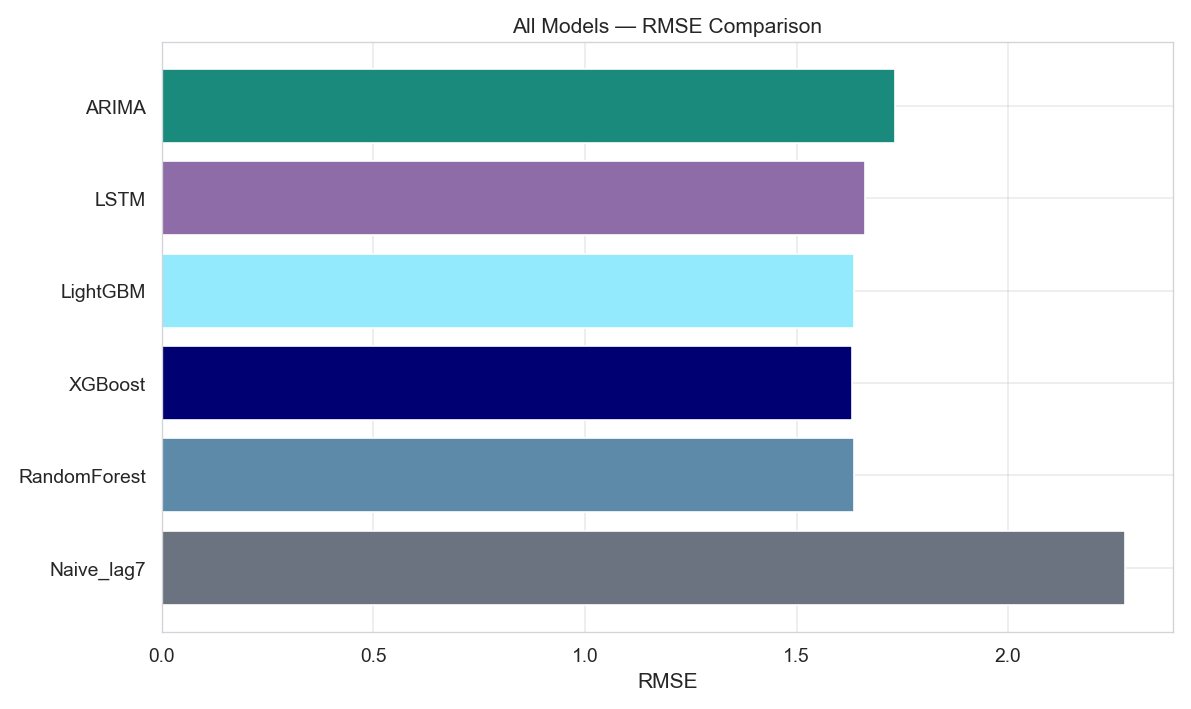
\includegraphics[width=0.85\textwidth]{figures/24_all_models_comparison.png}
\caption{Comparison of forecast accuracy (RMSE) across all six models. The three tree-based models form a tight cluster, substantially outperforming both classical and deep learning alternatives.}
\label{fig:all_models_comparison}
\end{figure}

ARIMA and LSTM occupy an intermediate position: both significantly outperform the naive baseline (RMSE reductions of 28.2\% and 27.7\% respectively) but fall short of the tree-based models. This result is consistent with the findings of the M5 forecasting competition \citep{makridakis2021m5findings}, where gradient boosting algorithms consistently outperformed both classical statistical methods and standalone deep learning approaches. The LSTM's slightly lower MAPE (49.8\%) but higher RMSE suggests it handles the zero-heavy distribution differently from tree models, producing fewer large percentage errors but occasionally larger absolute deviations.

\subsection{Comparison of Results Across Models}

\textbf{Promotional vs. non-promotional performance.} Table~\ref{tab:promo_results} compares model performance across demand segments:

\begin{table}[H]
\centering
\small
\caption{Model performance by demand segment (last validation fold).}
\label{tab:promo_results}
\begin{tabular}{|l|l|r|r|r|r|}
\hline
\textbf{Segment} & \textbf{Model} & \textbf{MAE} & \textbf{RMSE} & \textbf{MAPE (\%)} & \textbf{$\sigma_e$} \\
\hline
\multirow{4}{*}{Non-Promo} & XGBoost & 1.299 & 2.055 & 52.3 & 2.055 \\
 & LightGBM & 1.308 & 2.058 & 51.8 & 2.058 \\
 & Random Forest & 1.327 & 2.073 & 51.6 & 2.073 \\
 & Naive (lag-7) & 1.565 & 2.969 & 85.9 & 2.969 \\
\hline
\multirow{4}{*}{Promo} & XGBoost & 1.917 & 2.844 & 51.7 & 2.836 \\
 & LightGBM & 1.911 & 2.851 & 51.4 & 2.838 \\
 & Random Forest & 1.944 & 2.884 & 51.6 & 2.873 \\
 & Naive (lag-7) & 2.448 & 3.956 & 86.9 & 3.955 \\
\hline
\end{tabular}
\end{table}

Promotional demand is consistently harder to predict across all models, with RMSE values approximately 38\% higher than for non-promotional periods. However, the ML models maintain their advantage over the naive baseline in both segments, with RMSE improvements of approximately 28\% for non-promotional and 28\% for promotional demand.

\textbf{Per-product RMSE distribution.} Analysis at the individual product level reveals that LightGBM achieves a median per-product RMSE of 1.65, compared to 2.36 for the naive baseline. The improvement is not uniform: some products see RMSE reductions exceeding 15 units, while approximately 10 products show marginally worse performance with ML than with the naive approach. These products tend to have very low and stable demand where the simple lag-7 heuristic is already near-optimal.

\begin{figure}[H]
\centering
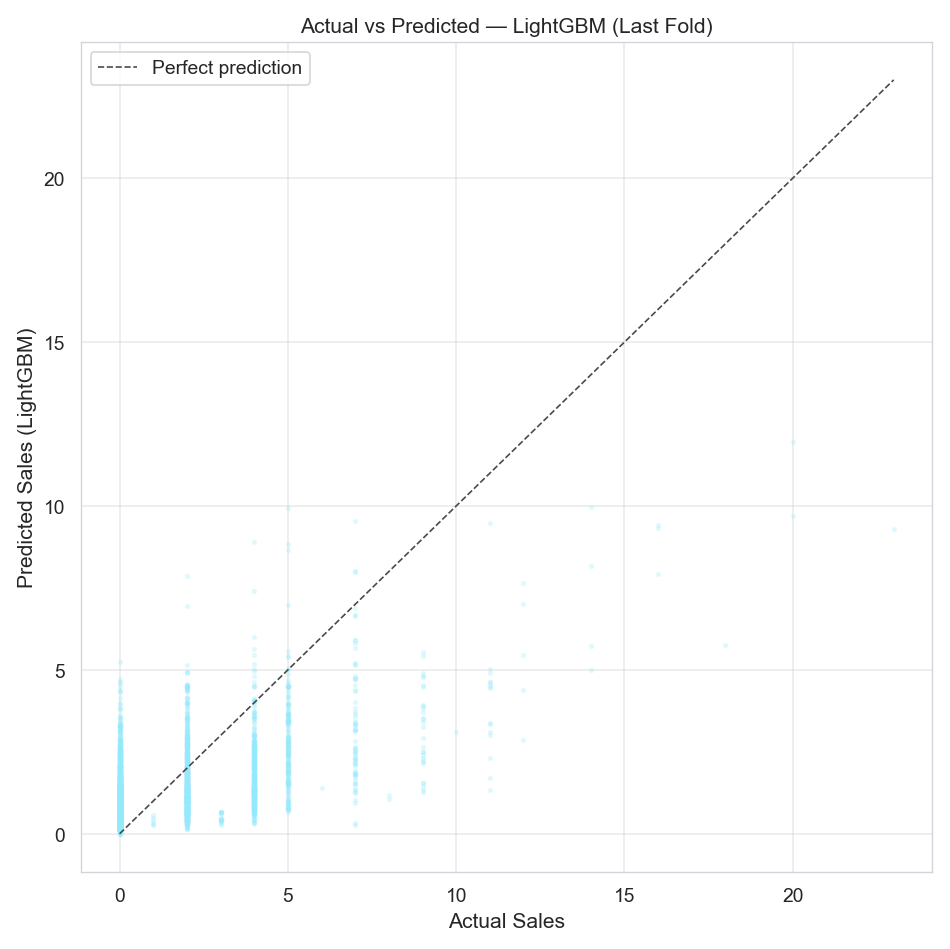
\includegraphics[width=0.85\textwidth]{figures/13_actual_vs_predicted_lgbm.png}
\caption{Actual vs.\ predicted sales for LightGBM on a sample of products. Points near the diagonal indicate accurate predictions; the cluster near the origin reflects the high proportion of zero-demand observations.}
\label{fig:actual_vs_predicted}
\end{figure}

\begin{figure}[H]
\centering
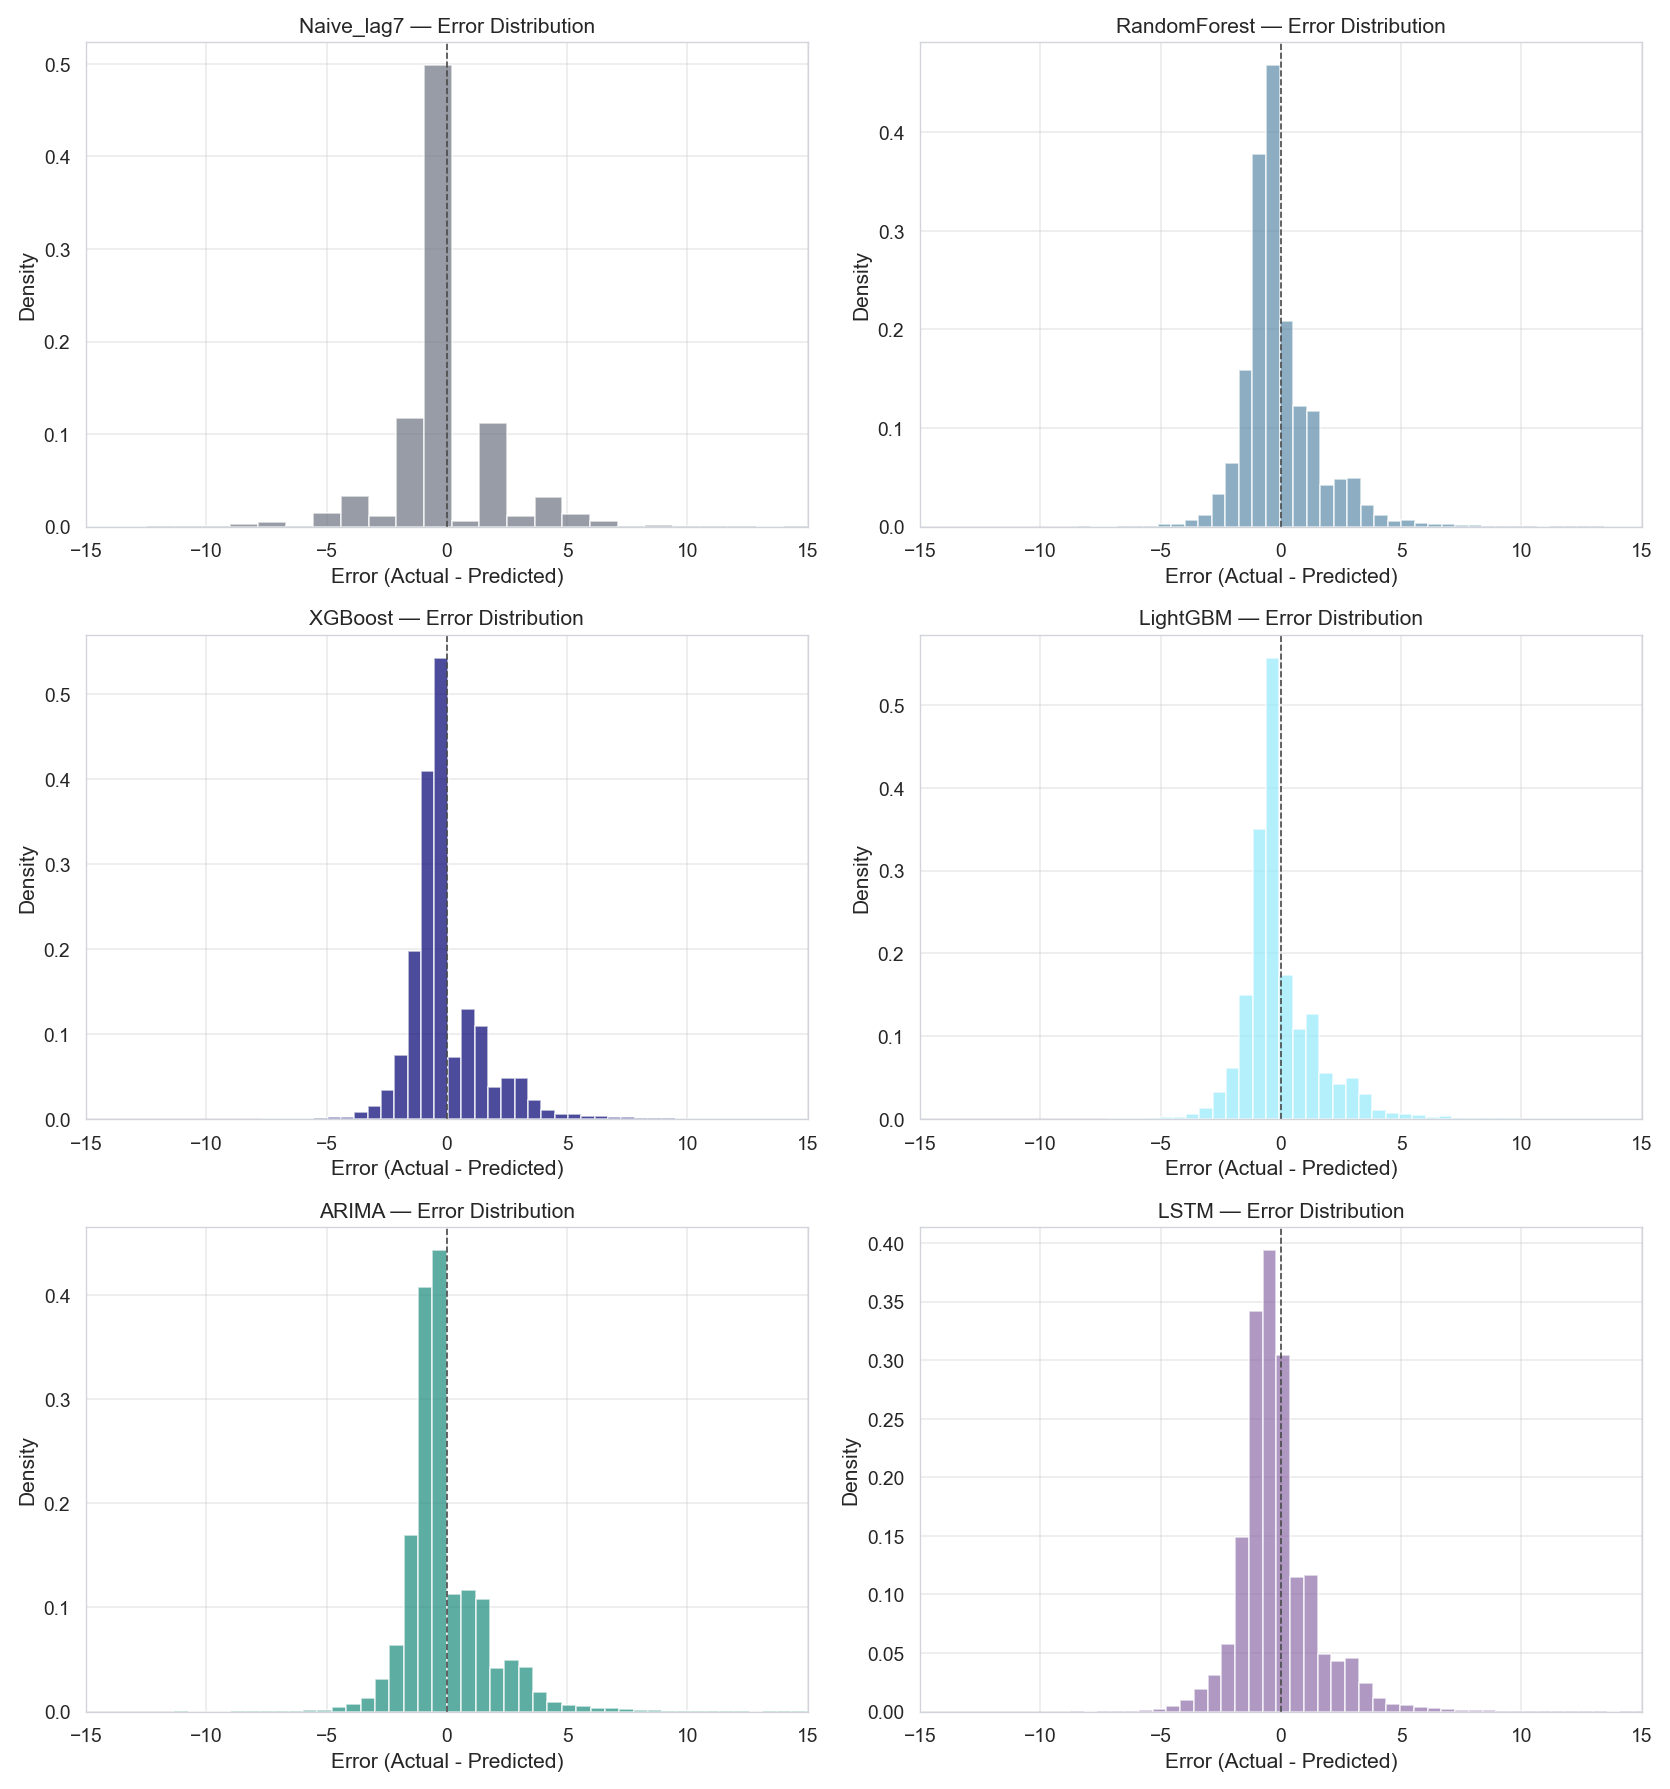
\includegraphics[width=0.85\textwidth]{figures/17_error_distributions.png}
\caption{Distribution of forecast errors by model. The ML models produce tighter, more symmetric error distributions compared to the naive baseline.}
\label{fig:error_distributions}
\end{figure}

\begin{figure}[H]
\centering
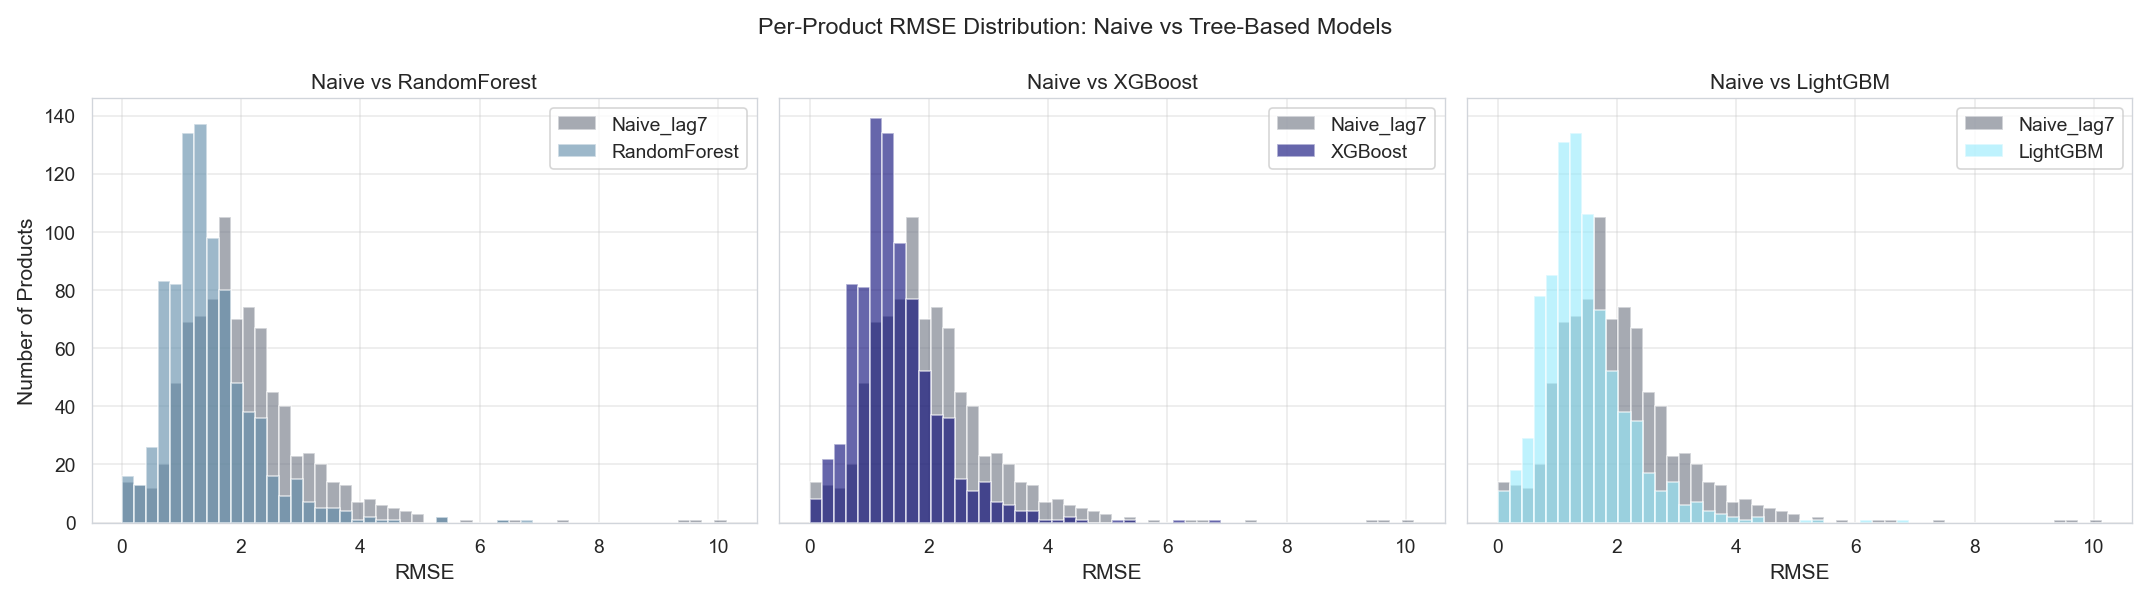
\includegraphics[width=0.85\textwidth]{figures/18_per_product_rmse_dist.png}
\caption{Distribution of per-product RMSE values. The ML models shift the distribution towards lower RMSE values compared to the naive baseline.}
\label{fig:per_product_rmse}
\end{figure}

\textbf{SHAP feature importance.} To understand the drivers of model predictions, SHAP (SHapley Additive exPlanations) analysis was performed on the LightGBM model. Table~\ref{tab:shap_top10} presents the ten most influential features:

\begin{table}[H]
\centering
\small
\caption{Top 10 features by mean absolute SHAP value (LightGBM).}
\label{tab:shap_top10}
\begin{tabular}{|r|l|r|}
\hline
\textbf{Rank} & \textbf{Feature} & \textbf{Mean $|$SHAP$|$} \\
\hline
1 & ewma\_28 & 0.524 \\
2 & bolHoliday & 0.295 \\
3 & roll\_mean\_28 & 0.150 \\
4 & day\_of\_week & 0.079 \\
5 & udsStock & 0.063 \\
6 & roll\_max\_28 & 0.046 \\
7 & lag\_28 & 0.025 \\
8 & bolOpen & 0.022 \\
9 & roll\_mean\_14 & 0.017 \\
10 & roll\_max\_14 & 0.016 \\
\hline
\end{tabular}
\end{table}

The 28-day EWMA emerges as the single most important predictor, followed by the holiday indicator and the 28-day rolling mean. This confirms that the model relies heavily on smoothed representations of recent demand history, with calendar effects providing secondary but significant predictive power. Notably, the longer-horizon features (28-day windows) dominate over shorter-horizon ones (7-day), suggesting that the model captures medium-term demand trends rather than relying solely on short-term momentum.

\begin{figure}[H]
\centering
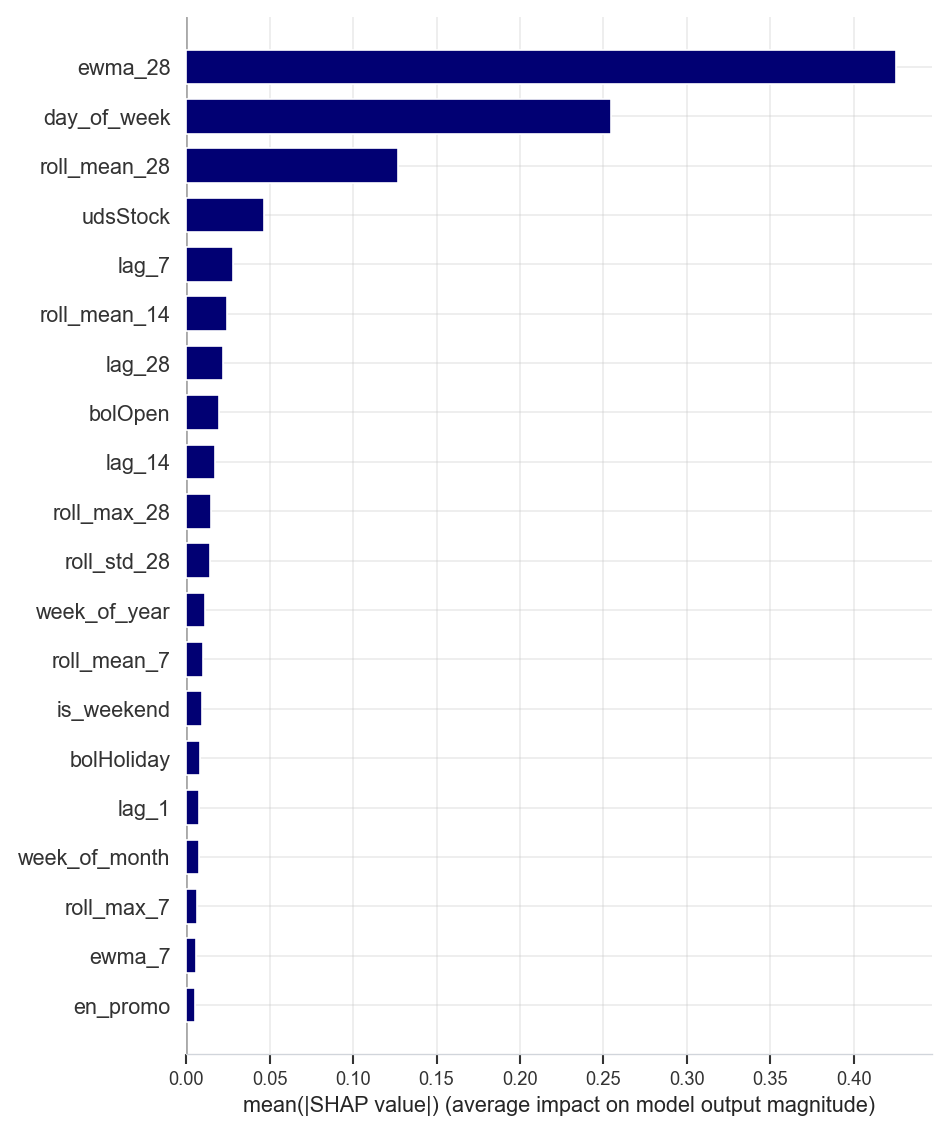
\includegraphics[width=0.85\textwidth]{figures/15_shap_bar.png}
\caption{SHAP feature importance (mean absolute SHAP values) for LightGBM. The 28-day EWMA dominates, followed by calendar and rolling statistics features.}
\label{fig:shap_bar}
\end{figure}

\begin{figure}[H]
\centering
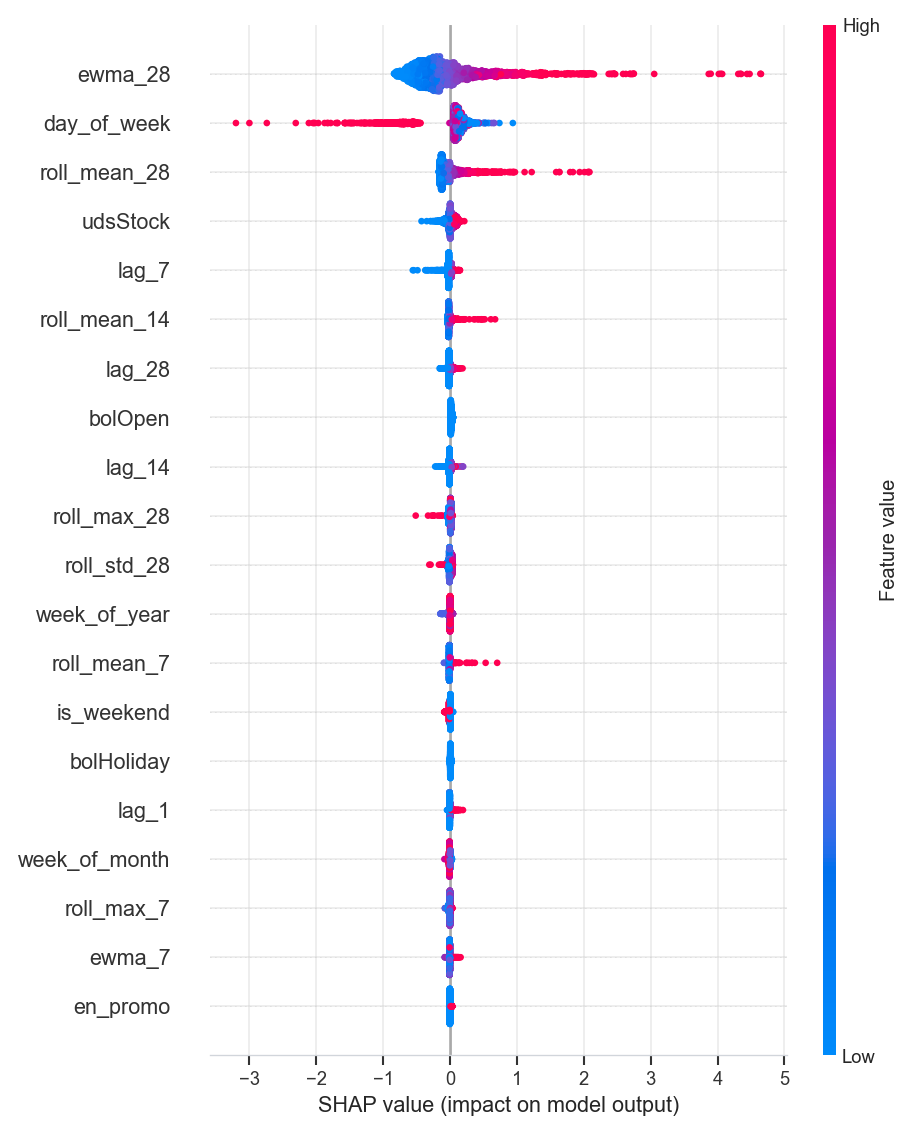
\includegraphics[width=0.85\textwidth]{figures/14_shap_summary.png}
\caption{SHAP summary plot showing the direction and magnitude of feature effects. Red indicates high feature values; blue indicates low values. High \texttt{ewma\_28} values push predictions upward, consistent with higher recent demand leading to higher forecasts.}
\label{fig:shap_summary}
\end{figure}

\subsection{Conclusions from Results}

The evaluation yields several key findings:

\begin{enumerate}
    \item The three tree-based machine learning models (XGBoost, LightGBM, Random Forest) achieve the best performance, with RMSE values within 1\% of each other. This suggests that the feature engineering, rather than the specific algorithm choice, is the primary driver of forecast quality among this model family.

    \item ARIMA and LSTM occupy an intermediate tier, both significantly outperforming the naive baseline (RMSE reductions of 28\% and 28\% respectively) but falling short of the tree-based models. ARIMA's per-product fitting captures local demand patterns effectively but cannot leverage cross-product information or engineered features. LSTM captures sequential dependencies but requires substantially more training data and computation to match tree-based performance.

    \item The improvement over the naive baseline is substantial across all ML approaches (28--30\% RMSE reduction), demonstrating the value of incorporating engineered features and systematic model training over simple heuristic forecasting.

    \item Promotional demand remains the most challenging segment, with RMSE approximately 38\% higher than non-promotional demand across all models. However, the ML models maintain their relative advantage over the baseline in both segments.

    \item SHAP analysis reveals that smoothed demand history (EWMA and rolling statistics) and calendar features are the most influential predictors, validating the feature engineering strategy adopted in this work.

    \item The forecast error standard deviation ($\sigma_e \approx 2.15$ for the best tree models, $\sigma_e \approx 2.22$ for ARIMA/LSTM, compared to $\sigma_e \approx 3.09$ for the naive baseline) translates directly into safety stock reductions, as quantified in the following section.
\end{enumerate}


\section{Impact of Algorithm Improvement}

\subsection{Impact on Processes}

The transition from a naive forecasting approach to machine learning models has implications beyond numerical accuracy improvements. From an operational perspective, the key process impacts are:

\textbf{Safety stock reduction.} Using the safety stock formulation from Equation~\ref{eq:safety_stock} with a 95\% service level ($z = 1.645$) and a protection period of 10 days (3 days lead time + 7 days review period), the total safety stock across all 894 products decreases from 11,953 units under the naive forecast to 8,276 units under LightGBM --- a reduction of 30.8\%. This means that the same service level can be maintained with significantly less inventory investment.

\textbf{Forecast error symmetry.} Analysis of error distributions shows that the ML models produce approximately symmetric errors centred near zero, whereas the naive baseline exhibits a slight positive bias (tendency to overforecast). Symmetric errors are preferable for inventory planning, as they indicate that the forecast is equally likely to overestimate or underestimate demand, allowing safety stock to function as intended.

\textbf{Sensitivity to service level.} Table~\ref{tab:sensitivity} presents the total safety stock requirements across different service levels:

\begin{table}[H]
\centering
\small
\caption{Total safety stock (units) by model and service level.}
\label{tab:sensitivity}
\begin{tabular}{|l|r|r|r|}
\hline
\textbf{Model} & \textbf{90\%} & \textbf{95\%} & \textbf{99\%} \\
\hline
LightGBM & 6,450 & 8,276 & 11,702 \\
XGBoost & 6,466 & 8,296 & 11,731 \\
Random Forest & 6,507 & 8,350 & 11,806 \\
Naive (lag-7) & 9,316 & 11,953 & 16,902 \\
\hline
\end{tabular}
\end{table}

The ML models consistently require approximately 30\% less safety stock than the naive baseline across all service levels, demonstrating that the improvement is robust and not dependent on a specific service level assumption.

\begin{figure}[H]
\centering
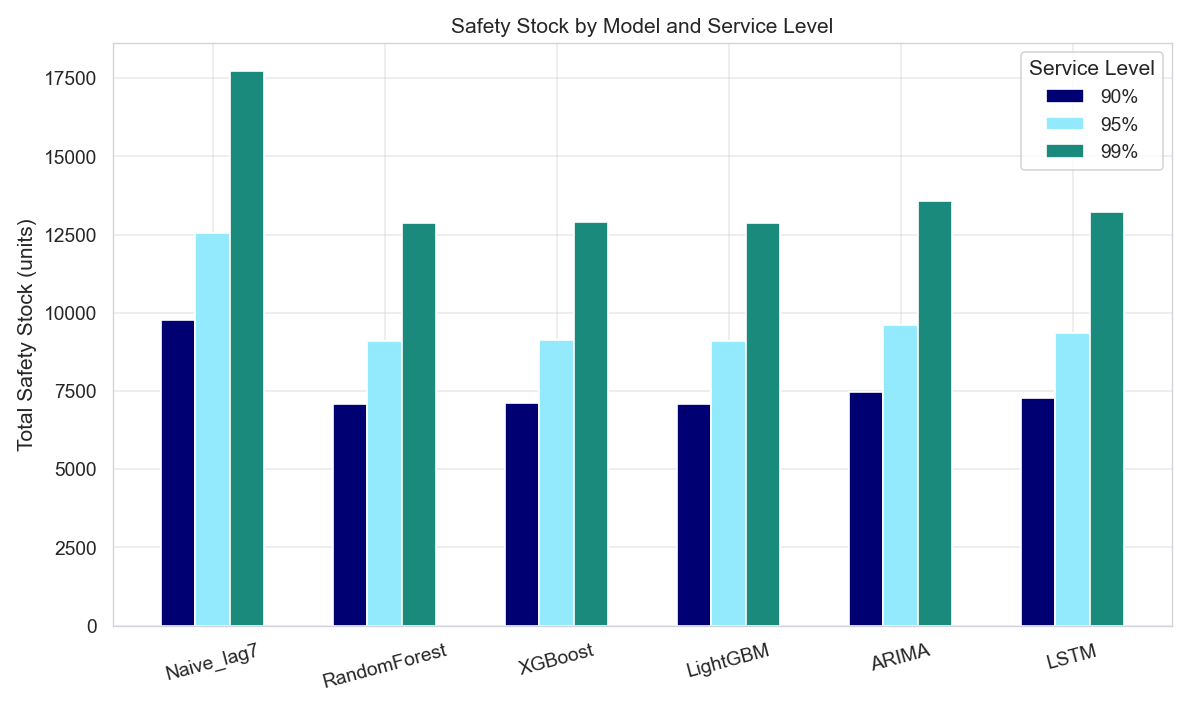
\includegraphics[width=0.85\textwidth]{figures/21_safety_stock_by_service_level.png}
\caption{Total safety stock requirements by model and service level. The ML models maintain a consistent ~30\% advantage over the naive baseline across all service levels.}
\label{fig:safety_stock_service_level}
\end{figure}

\subsection{Economic Impact}

The economic impact analysis combines two cost components: the newsvendor cost (direct cost of forecast errors) and the safety stock holding cost.

\textbf{Newsvendor cost analysis.} Following the total cost formulation from Equation~\ref{eq:total_cost}, the asymmetric costs of overforecasting and underforecasting were computed using cost parameters of $C_o = \text{\euro}0.10$ per unit per day (overage/holding) and $C_u = \text{\euro}0.50$ per unit per day (underage/lost sale), yielding a critical ratio of 0.83. These values reflect a typical retail/industrial setting where stockout costs substantially exceed holding costs.

Table~\ref{tab:newsvendor} presents the newsvendor cost results:

\begin{table}[H]
\centering
\small
\caption{Newsvendor cost analysis (30-day test period, annualised).}
\label{tab:newsvendor}
\begin{tabular}{|l|r|r|r|r|}
\hline
\textbf{Model} & \textbf{Overage (€)} & \textbf{Underage (€)} & \textbf{Total (€)} & \textbf{Annual est. (€)} \\
\hline
Naive (lag-7) & 2,227 & 11,138 & 13,365 & 162,603 \\
Random Forest & 1,830 & 9,538 & 11,367 & 138,304 \\
LightGBM & 1,786 & 9,489 & 11,275 & 137,182 \\
XGBoost & 1,785 & 9,392 & 11,176 & 135,979 \\
\hline
\end{tabular}
\end{table}

XGBoost achieves the lowest newsvendor cost, saving approximately \euro26,600 annually (16.4\%) compared to the naive baseline. Underage costs dominate in all models, consistent with the asymmetric cost structure where stockouts are five times more expensive than excess inventory.

\textbf{Combined cost analysis.} Table~\ref{tab:combined_cost} presents the total annual cost combining newsvendor costs with safety stock holding costs at the 95\% service level:

\begin{table}[H]
\centering
\small
\caption{Combined annual cost: newsvendor + safety stock holding (95\% service level).}
\label{tab:combined_cost}
\begin{tabular}{|l|r|r|r|}
\hline
\textbf{Model} & \textbf{Newsvendor (€/yr)} & \textbf{SS Holding (€/yr)} & \textbf{Total (€/yr)} \\
\hline
Naive (lag-7) & 162,603 & 436,294 & 598,896 \\
Random Forest & 138,304 & 304,763 & 443,067 \\
LightGBM & 137,182 & 302,083 & 439,265 \\
XGBoost & 135,979 & 302,816 & 438,796 \\
\hline
\end{tabular}
\end{table}

The ML models achieve total annual cost savings of approximately \euro160,000 (26.7\%) compared to the naive baseline. XGBoost and LightGBM perform nearly identically in economic terms, with XGBoost holding a marginal advantage of \euro469 annually.

\begin{figure}[H]
\centering
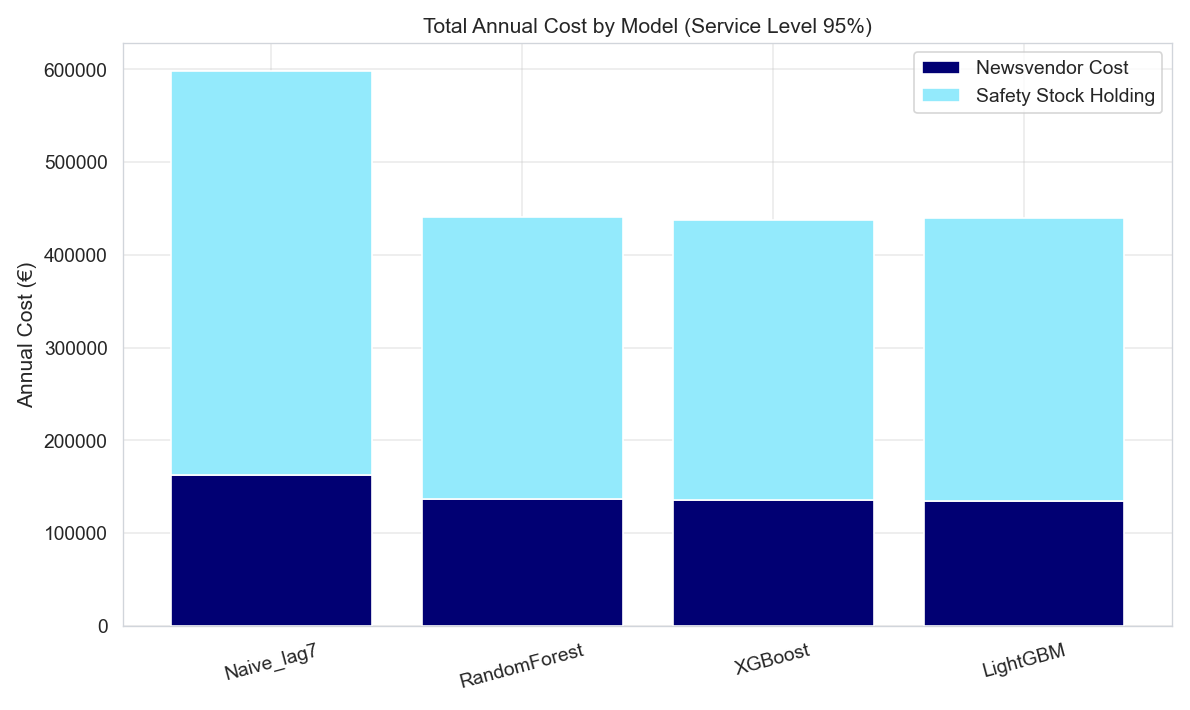
\includegraphics[width=0.85\textwidth]{figures/22_combined_annual_cost.png}
\caption{Combined annual inventory cost (newsvendor + safety stock holding) by model. The ML models reduce total costs by approximately 26.7\% compared to the naive baseline.}
\label{fig:combined_annual_cost}
\end{figure}

These results demonstrate that the forecast accuracy improvements documented in Section~3.6 translate into meaningful economic benefits. The 28\% reduction in RMSE corresponds to a 26.7\% reduction in total inventory-related costs, confirming the theoretical relationship between forecast error and inventory costs established in Chapter~2 (Equations~\ref{eq:ss_cost} and \ref{eq:total_cost}).

It is important to note that the cost parameters used in this analysis ($C_o$ and $C_u$) are illustrative values chosen to reflect typical industrial cost structures. The relative ranking of models and the percentage savings are robust to reasonable variations in these parameters, as the underlying driver is the reduction in forecast error rather than the specific cost assumptions. A sensitivity analysis across service levels (Table~\ref{tab:sensitivity}) confirms that the ML advantage is maintained regardless of the risk tolerance adopted by the organisation.
 in TFM_onamas.tex

This chapter presents the complete design and implementation of the demand forecasting system, following the CRISP-DM methodology introduced in Chapter~1. The work progresses from data acquisition and exploration through preprocessing, feature engineering, model development, evaluation, and finally the economic impact analysis that connects forecast accuracy to inventory cost savings.

\section{Data Origin}

\subsection{Data Acquisition}

The dataset used in this project was provided by the thesis supervisor and corresponds to real historical data from a company operating in the automotive sector. The data covers daily demand records for a portfolio of products, along with supplementary information on calendar events, promotional campaigns, and stock levels. All data was received in a single Microsoft Excel file (\texttt{Datos.xlsx}) containing four sheets, each representing a distinct dimension of the business context.

No personally identifiable information is present in the dataset, and all product references are anonymised using numerical identifiers, ensuring compliance with data privacy requirements as discussed in Section~\ref{s:etic}.

\subsection{Data Description}

The dataset comprises four tables, summarised in Table~\ref{tab:data_sheets}:

\begin{table}[H]
\centering
\small
\caption{Structure of the source dataset (\texttt{Datos.xlsx}).}
\label{tab:data_sheets}
\begin{tabular}{|l|l|r|p{5.5cm}|}
\hline
\textbf{Sheet} & \textbf{Key columns} & \textbf{Rows} & \textbf{Description} \\
\hline
Ventas (Sales) & producto, fecha, udsVenta & 654,588 & Daily unit sales per product \\
\hline
Calendario & fecha, bolOpen, bolHoliday & 732 & Calendar flags: business day and holiday indicators \\
\hline
Promociones & producto, fechaInicio, fechaFin & 1,894 & Promotional campaign periods per product \\
\hline
Stock & producto, fecha, udsStock & 654,588 & Daily stock levels per product \\
\hline
\end{tabular}
\end{table}

The sales sheet constitutes the core of the dataset, containing 654,588 daily observations across 894 unique products over a period of 732 days, spanning from November 2022 to November 2024. Each record represents the number of units sold for a specific product on a specific date.

The calendar sheet provides 732 daily records with two binary indicators: \texttt{bolOpen} (whether the business was open) and \texttt{bolHoliday} (whether the date was a public holiday). The promotions sheet contains 1,894 records defining promotional campaign windows through start and end dates for each product. The stock sheet mirrors the sales structure, recording the closing stock level for each product-date combination.

\subsection{Data Loading}

All four sheets were loaded into memory using the \texttt{pandas} library with the \texttt{openpyxl} engine. The sales and stock tables were merged on the shared keys \texttt{(producto, fecha)}, and the calendar information was joined on \texttt{fecha}. Promotional periods were transformed from date ranges into a binary indicator (\texttt{en\_promo}) at the product-date level, marking each observation as promotional or non-promotional based on whether the date fell within any active campaign for that product.

After merging, the resulting dataset contained 654,588 rows and served as the foundation for all subsequent analysis. The merged dataset was persisted in Apache Parquet format for efficient reloading in downstream scripts.


\section{Data Exploration}

\subsection{Data Summary}

An initial statistical summary of the target variable (\texttt{udsVenta}, units sold) revealed a highly skewed distribution. The mean daily sales per product were 1.42 units, with a median of zero and a standard deviation of 3.56. The maximum observed value was 99 units. This distribution reflects the nature of automotive parts demand, where the majority of product-day combinations register zero sales, punctuated by occasional larger orders.

Table~\ref{tab:sales_stats} presents the key descriptive statistics:

\begin{table}[H]
\centering
\small
\caption{Descriptive statistics of daily unit sales (\texttt{udsVenta}).}
\label{tab:sales_stats}
\begin{tabular}{|l|r|}
\hline
\textbf{Statistic} & \textbf{Value} \\
\hline
Count & 654,588 \\
Mean & 1.42 \\
Std. deviation & 3.56 \\
Median (50\%) & 0.00 \\
75th percentile & 1.00 \\
95th percentile & 7.00 \\
Maximum & 99 \\
Zero-sales proportion & 64.5\% \\
\hline
\end{tabular}
\end{table}

The high proportion of zero-sales observations (64.5\%) is a defining characteristic of this dataset and has important implications for model selection and evaluation, as discussed in subsequent sections.

\begin{figure}[H]
\centering
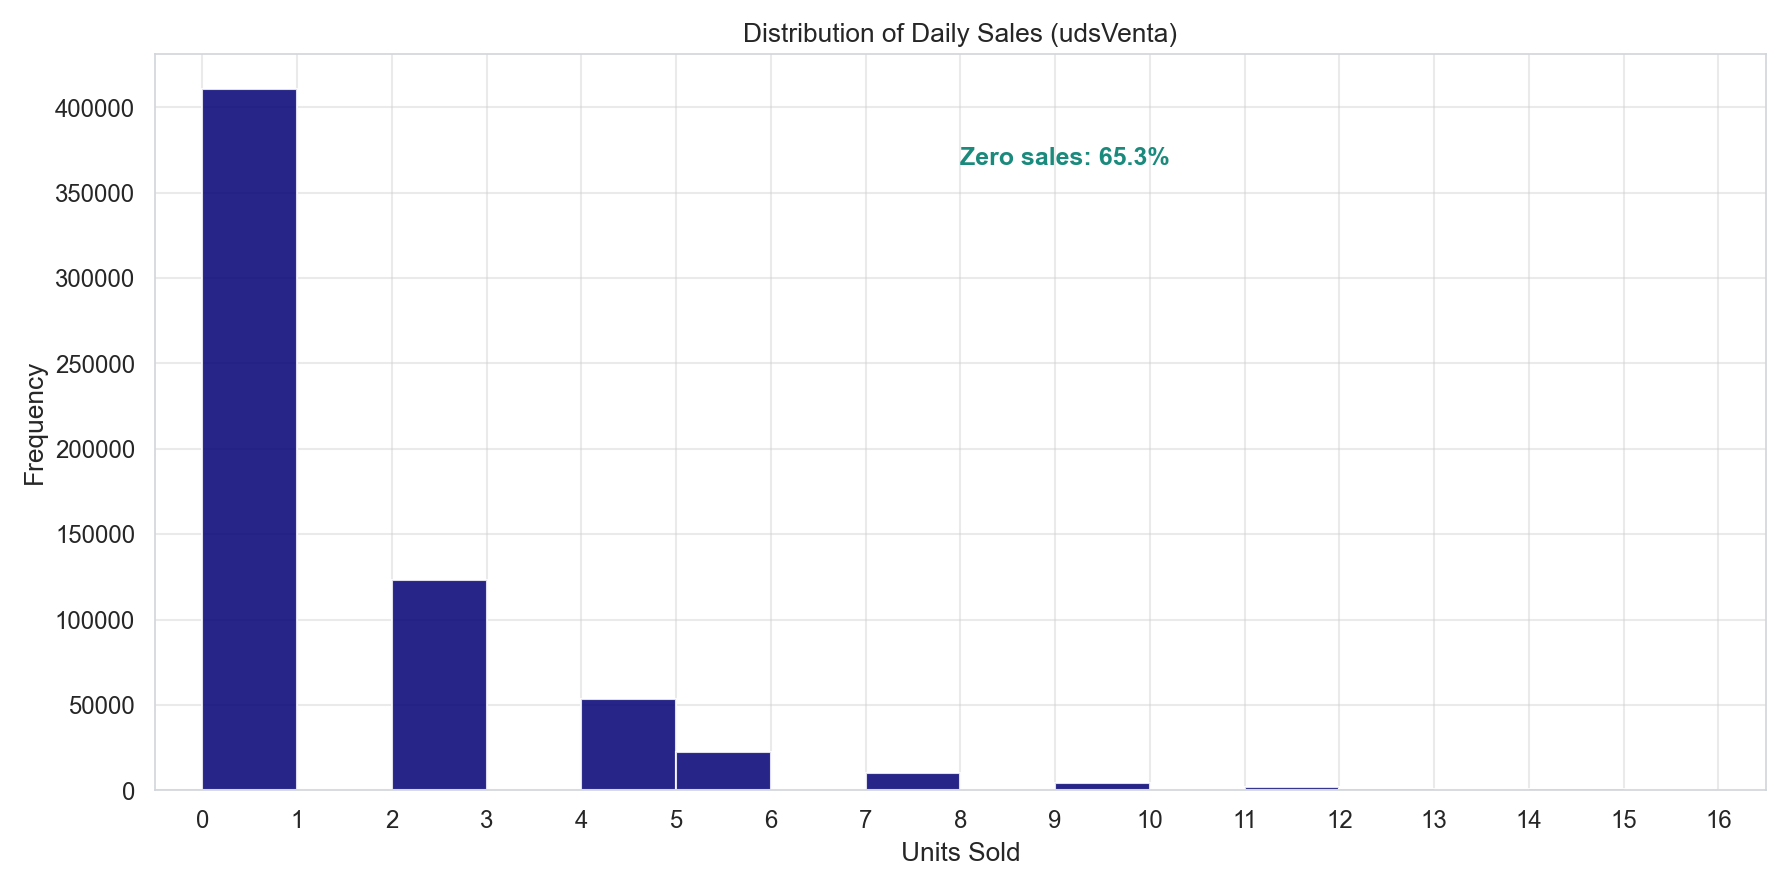
\includegraphics[width=0.85\textwidth]{figures/01_sales_distribution.png}
\caption{Distribution of daily unit sales (\texttt{udsVenta}). The histogram confirms the extreme right skew, with the majority of observations at zero.}
\label{fig:sales_distribution}
\end{figure}

\subsection{Statistical Analysis}

The exploratory analysis examined demand patterns across several dimensions:

\textbf{Day-of-week patterns.} Sales exhibit a clear weekly cycle, with the highest volumes on weekdays (Monday through Friday) and a sharp decline on Saturdays. Sunday sales are near zero, consistent with the business being closed on Sundays as indicated by the \texttt{bolOpen} calendar flag. This weekly seasonality motivates the inclusion of day-of-week features and the use of a lag-7 naive baseline (same weekday, previous week) as the primary benchmark.

\begin{figure}[H]
\centering
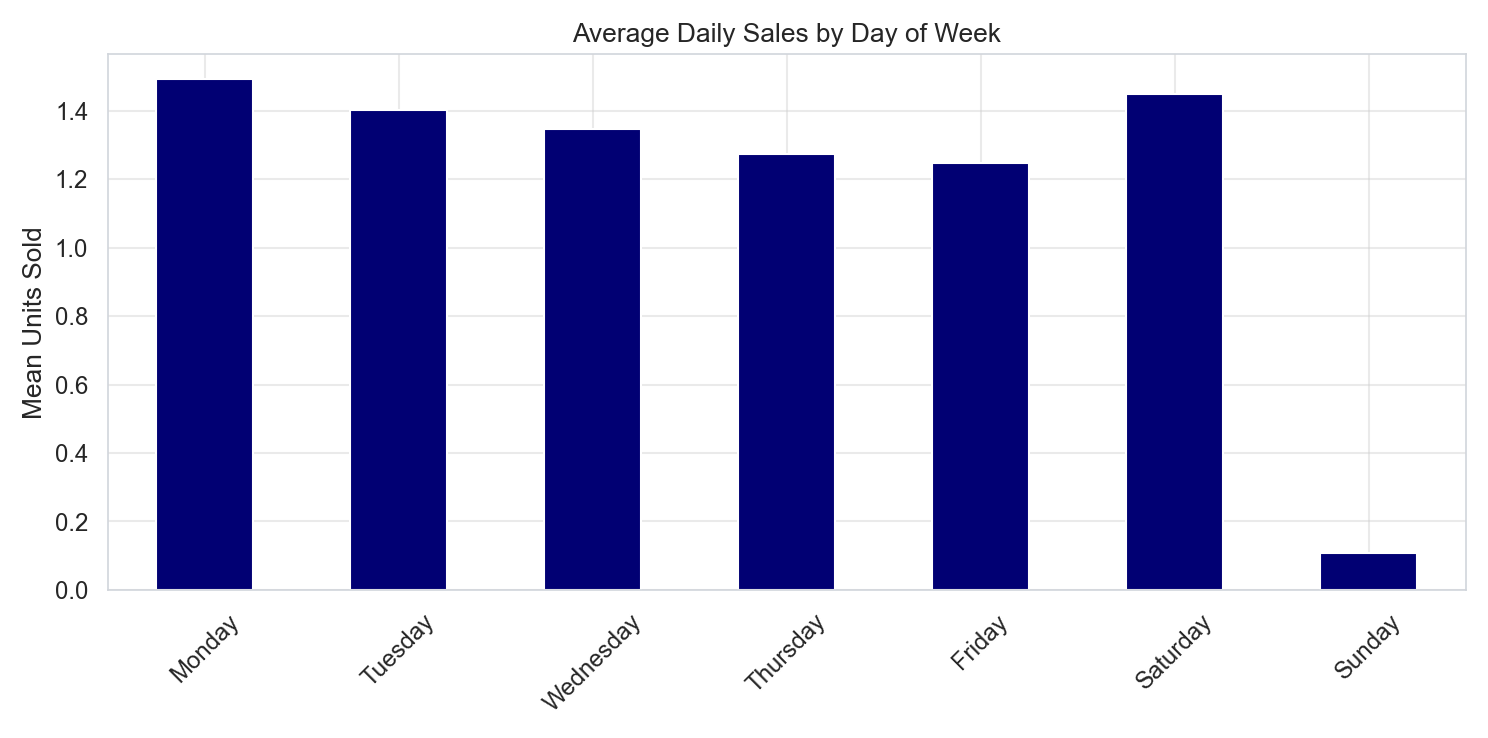
\includegraphics[width=0.85\textwidth]{figures/02_sales_by_day_of_week.png}
\caption{Average daily sales by day of the week. The weekly cycle is clearly visible, with near-zero sales on Sundays.}
\label{fig:sales_by_dow}
\end{figure}

\textbf{Monthly and seasonal patterns.} Monthly aggregated sales show moderate variation across the year, without a single dominant seasonal peak. However, certain months consistently show higher activity, suggesting that calendar-based features (month, week of year) may contribute predictive value.

\textbf{Promotional effects.} Comparing sales during promotional and non-promotional periods revealed that mean sales during promotions (1.83 units) were slightly higher than during non-promotional periods (1.38 units). However, the difference is modest, and the promotional flag alone does not capture the full complexity of promotional demand dynamics, which motivated the engineering of additional promotional features described in Section~3.4.

\begin{figure}[H]
\centering
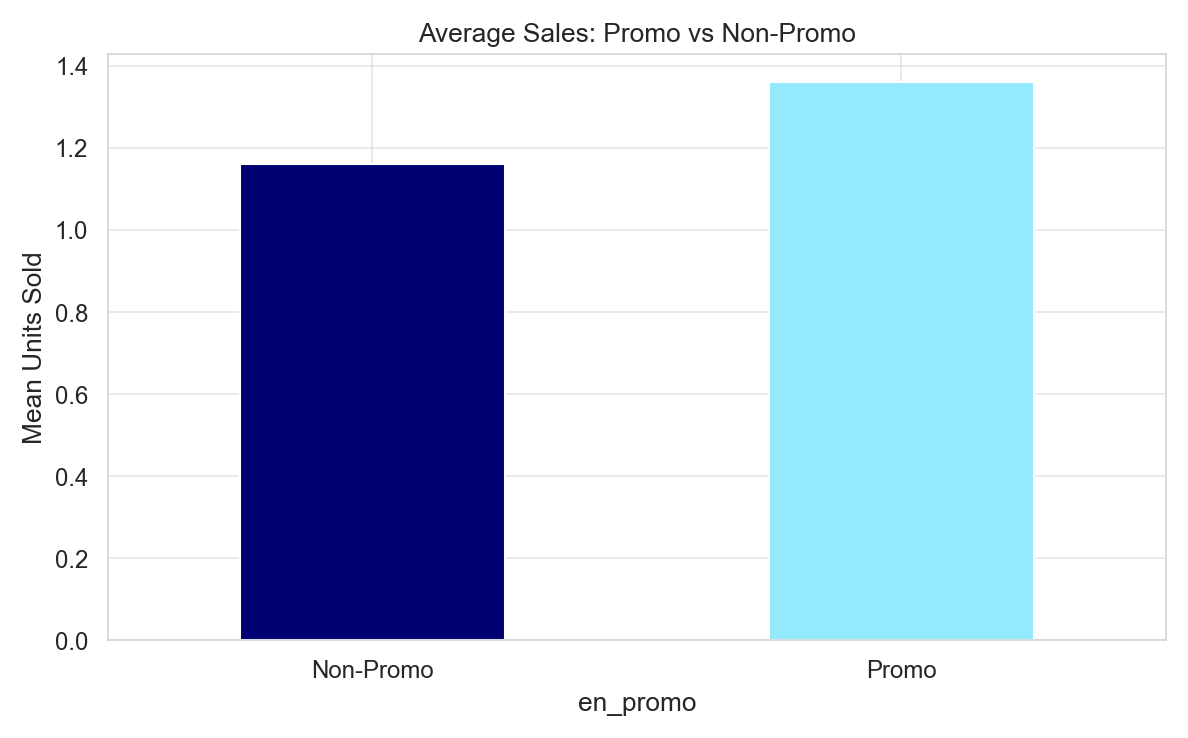
\includegraphics[width=0.85\textwidth]{figures/05_promo_vs_nonpromo.png}
\caption{Comparison of sales distributions during promotional and non-promotional periods.}
\label{fig:promo_vs_nonpromo}
\end{figure}

\textbf{Autocorrelation structure.} Autocorrelation analysis on a sample of products confirmed significant positive autocorrelation at lags 1, 7, 14, and 28, with the strongest signal at lag 7 (weekly periodicity). This finding directly supports the creation of lag features at these intervals and validates the choice of lag-7 as the naive baseline.

\begin{figure}[H]
\centering
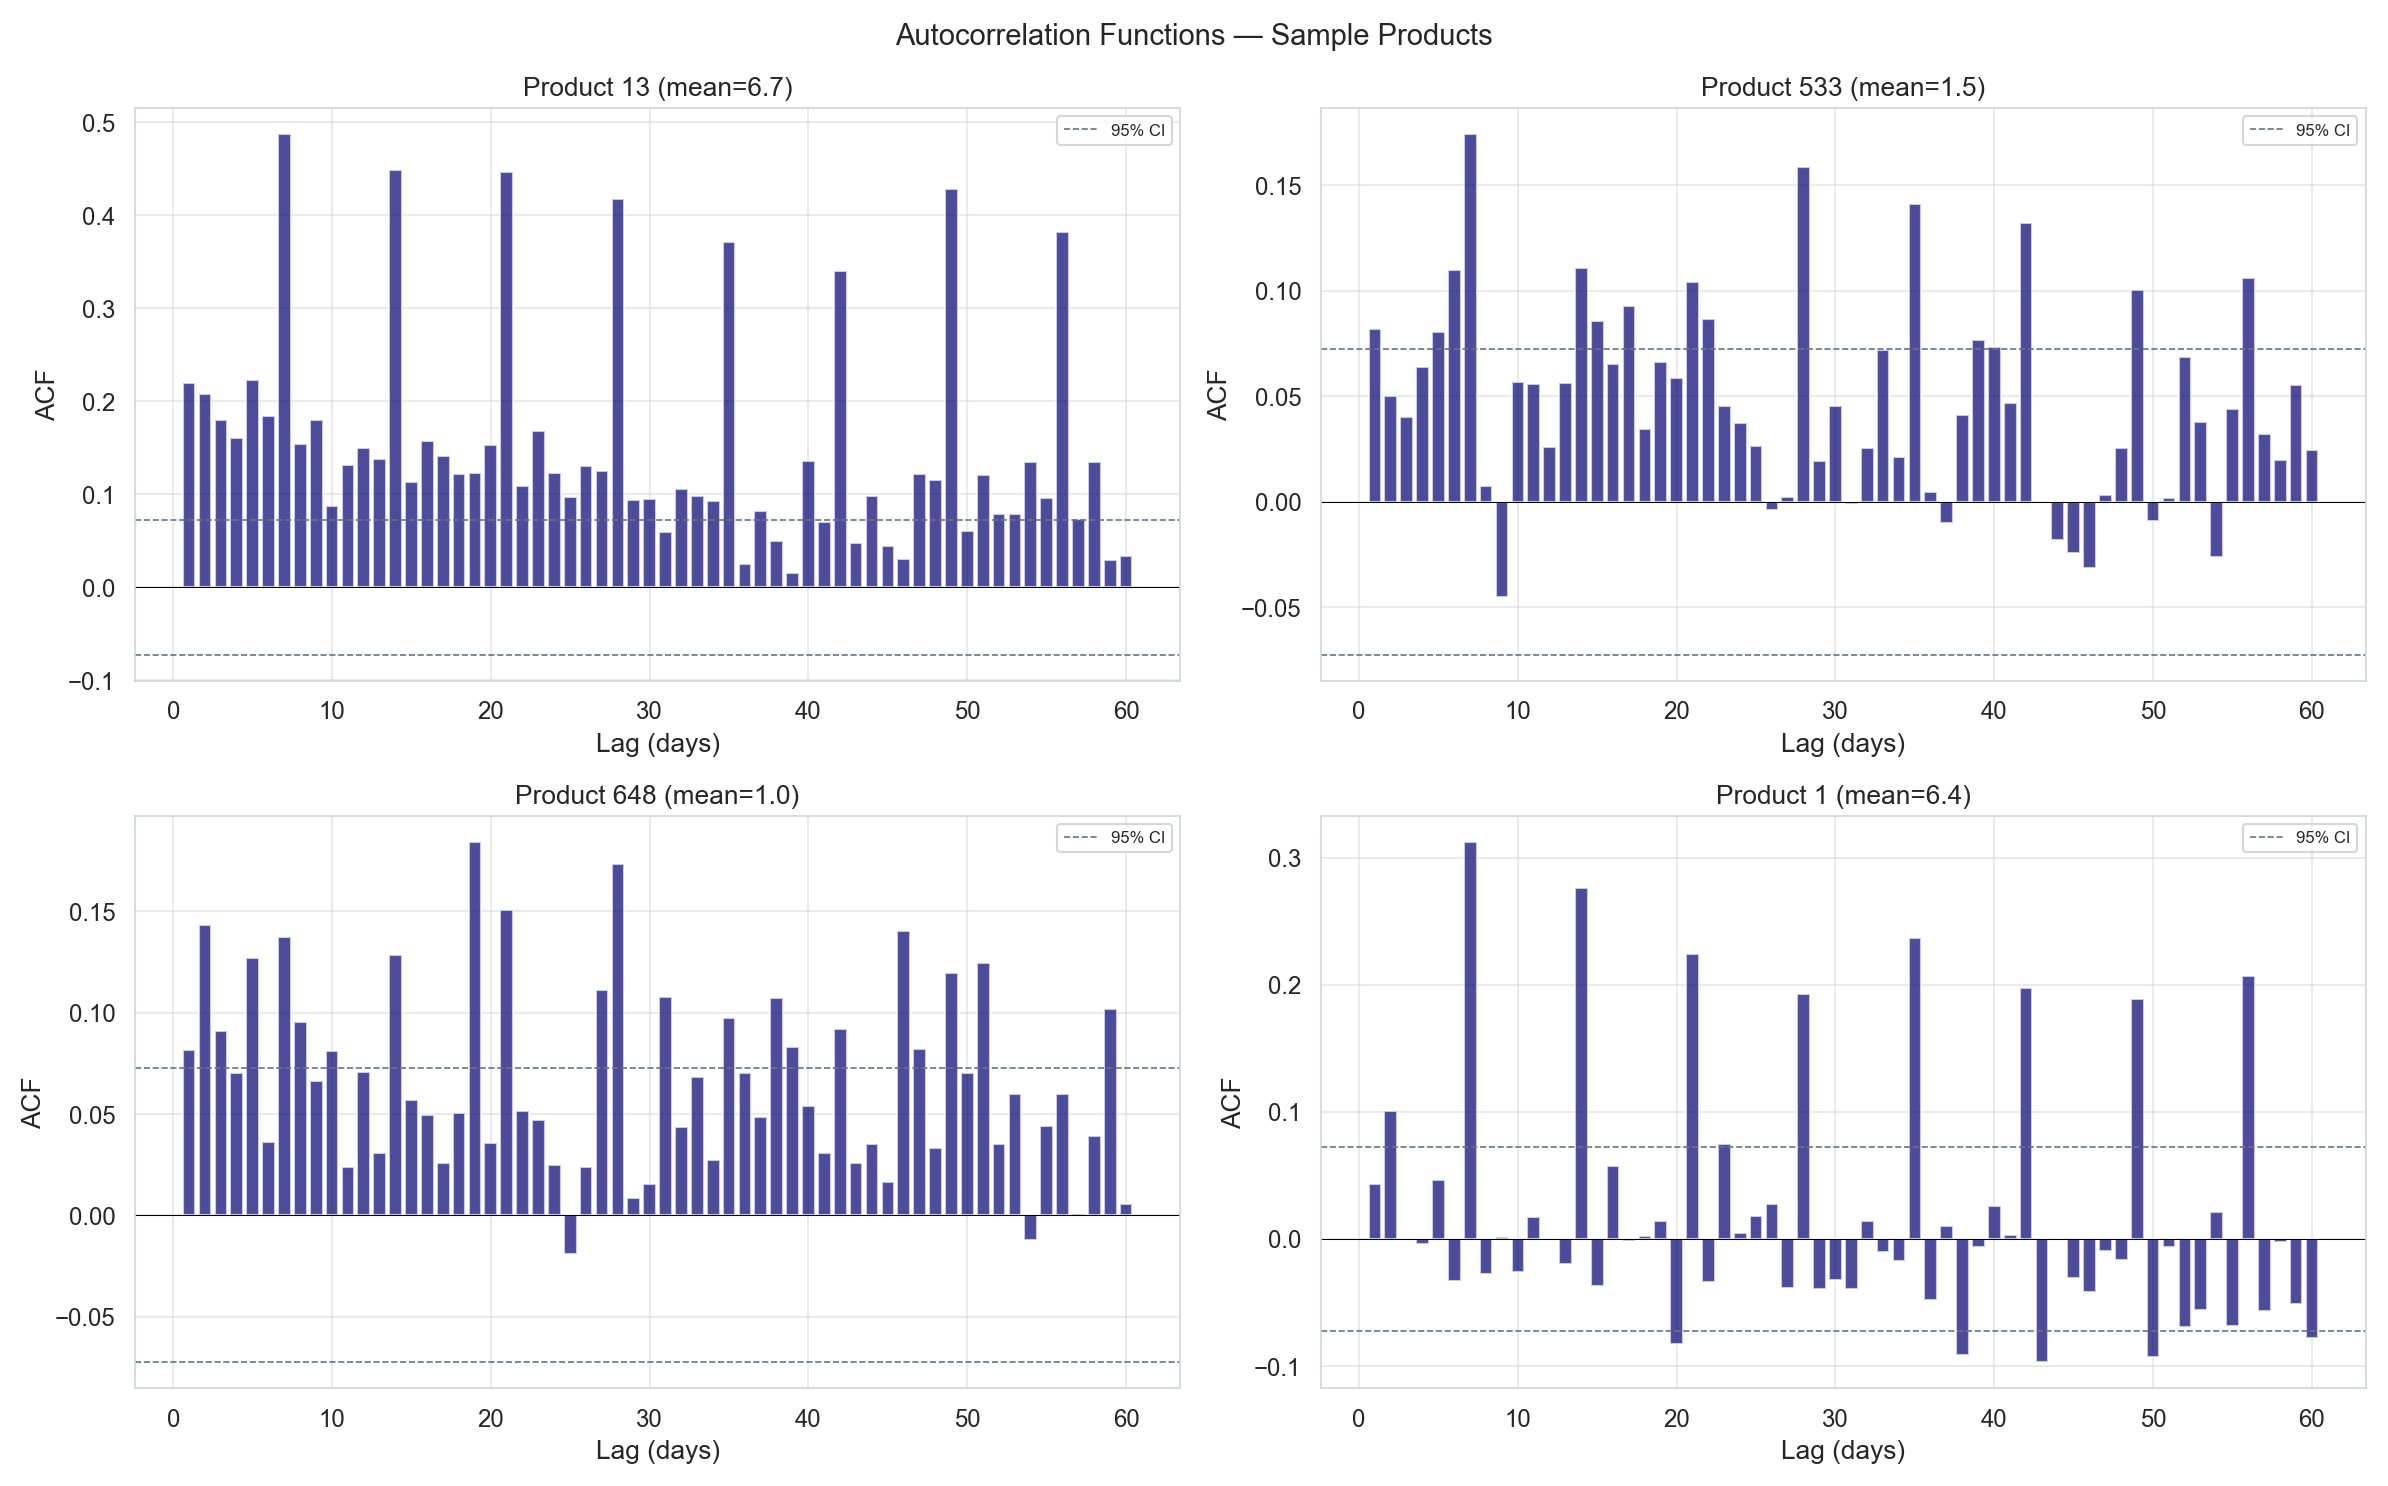
\includegraphics[width=0.85\textwidth]{figures/08_autocorrelation_sample.png}
\caption{Autocorrelation function (ACF) for a sample of products, showing significant positive autocorrelation at weekly intervals.}
\label{fig:autocorrelation}
\end{figure}

\subsection{Data Quality Analysis}

The data quality assessment identified the following issues:

\textbf{Missing values.} No explicit missing values were found in any of the four source tables. However, implicit gaps exist where lag features cannot be computed for the earliest dates in each product's history (addressed during feature engineering).

\textbf{Negative values.} No negative sales or stock values were present in this dataset.

\textbf{Stock breaks.} A stock break is defined as a day where both sales and stock are zero, potentially indicating that demand existed but could not be fulfilled due to inventory unavailability. Approximately 3.9\% of observations met this criterion. These were treated during data cleaning by imputing the product's historical mean sales for the corresponding weekday.

\textbf{Outliers.} Outlier detection was performed using a threshold of 1.75 times the interquartile range (IQR) per product. This identified approximately 11,400 observations (1.75\% of the dataset) as outliers, which were capped at the upper threshold value. The IQR-based approach was preferred over a fixed standard deviation threshold to account for the varying demand scales across products.


\section{Data Preparation}

\subsection{Data Cleaning}

The data cleaning process addressed the two quality issues identified during exploration:

\begin{enumerate}
    \item \textbf{Stock break imputation:} For observations where both \texttt{udsVenta} and \texttt{udsStock} were zero, the sales value was replaced with the mean sales for that product on the same weekday, computed over the preceding 30 days. This approach assumes that zero sales on a day with zero stock reflects a supply-side constraint rather than genuine zero demand, and uses a localised historical average to provide a reasonable demand estimate.

    \item \textbf{Outlier capping:} Values exceeding 1.75 $\times$ IQR above the 75th percentile for each product were capped at the threshold value. This preserves the general distribution shape while limiting the influence of extreme observations on model training. A total of 11,400 values (1.75\% of the dataset) were capped.
\end{enumerate}

After cleaning, the dataset retained its original 654,588 rows with no records removed, ensuring that the temporal continuity required for lag feature computation was preserved.

\subsection{Data Transformation}

The date column (\texttt{fecha}) was parsed into a \texttt{datetime} type, and the dataset was sorted by product and date to ensure correct temporal ordering for all subsequent operations. The promotional periods from the source data were transformed from date-range format into a daily binary indicator (\texttt{en\_promo}), assigned at the product-date level.

No logarithmic or power transformations were applied to the target variable. While such transformations can stabilise variance in skewed distributions, the tree-based models used in this work (Random Forest, XGBoost, LightGBM) are inherently robust to non-normal distributions and do not require target transformation for effective learning.

\subsection{Data Scaling}

Feature scaling (standardisation or normalisation) was not applied for the tree-based models, as decision tree ensembles are invariant to monotonic transformations of input features. The split-based learning mechanism of these algorithms operates on feature rankings rather than absolute values, making scaling unnecessary.

For the LSTM model, min-max normalisation was applied to all input features to facilitate gradient-based optimisation. Each feature was scaled to the $[0, 1]$ range using the training set statistics, and the same transformation was applied to the validation and test sets to prevent information leakage. Predictions were inverse-transformed back to the original scale before computing evaluation metrics.

\section{Feature Engineering}

Feature engineering is a central component of this work. A comprehensive set of 36 engineered features was designed to capture temporal dependencies, demand dynamics, and promotional effects. The features are organised into five categories, summarised in Table~\ref{tab:features}.

\begin{table}[H]
\centering
\small
\caption{Engineered features by category.}
\label{tab:features}
\begin{tabular}{|l|p{7cm}|r|}
\hline
\textbf{Category} & \textbf{Features} & \textbf{Count} \\
\hline
Original variables & udsStock, bolOpen, bolHoliday, en\_promo & 4 \\
\hline
Calendar features & year, month, day\_of\_week, week\_of\_year, week\_of\_month, is\_weekend, is\_month\_start, is\_month\_end & 8 \\
\hline
Lag features & lag\_1, lag\_7, lag\_14, lag\_28 & 4 \\
\hline
Rolling statistics & roll\_mean/std/min/max at 7, 14, and 28-day windows; ewma\_7, ewma\_28 & 14 \\
\hline
Promotional features & days\_since\_promo\_end, post\_promo\_7d, promo\_x\_lag7 & 3 \\
\hline
Product-level statistics & prod\_mean\_sales, prod\_std\_sales, prod\_median\_sales & 3 \\
\hline
\multicolumn{2}{|r|}{\textbf{Total}} & \textbf{36} \\
\hline
\end{tabular}
\end{table}

\textbf{Lag features} capture the autoregressive structure identified during exploration. The lag-7 feature (same weekday, previous week) serves dual purpose: it is used directly as the naive baseline forecast and as an input feature for the machine learning models. Lags at 1, 14, and 28 days capture short-term momentum, biweekly patterns, and monthly cycles respectively.

\textbf{Rolling statistics} provide smoothed representations of recent demand behaviour. For each window size (7, 14, and 28 days), the mean, standard deviation, minimum, and maximum of past sales are computed. Additionally, exponentially weighted moving averages (EWMA) with spans of 7 and 28 days provide adaptive smoothing that gives greater weight to more recent observations.

\textbf{Promotional features} go beyond the binary indicator to capture the temporal dynamics of promotions. The \texttt{days\_since\_promo\_end} feature tracks the recency of the last promotional period, \texttt{post\_promo\_7d} flags the week immediately following a promotion (to capture post-promotional demand depression), and \texttt{promo\_x\_lag7} is an interaction term between the promotional flag and the lag-7 sales value.

All lag and rolling features were computed strictly using past data to prevent information leakage. Observations where lag features could not be computed (the first 28 days of each product's history) were dropped, reducing the dataset from 654,588 to 629,370 rows. The final feature matrix was saved in Parquet format for use in the modelling phase.

\begin{figure}[H]
\centering
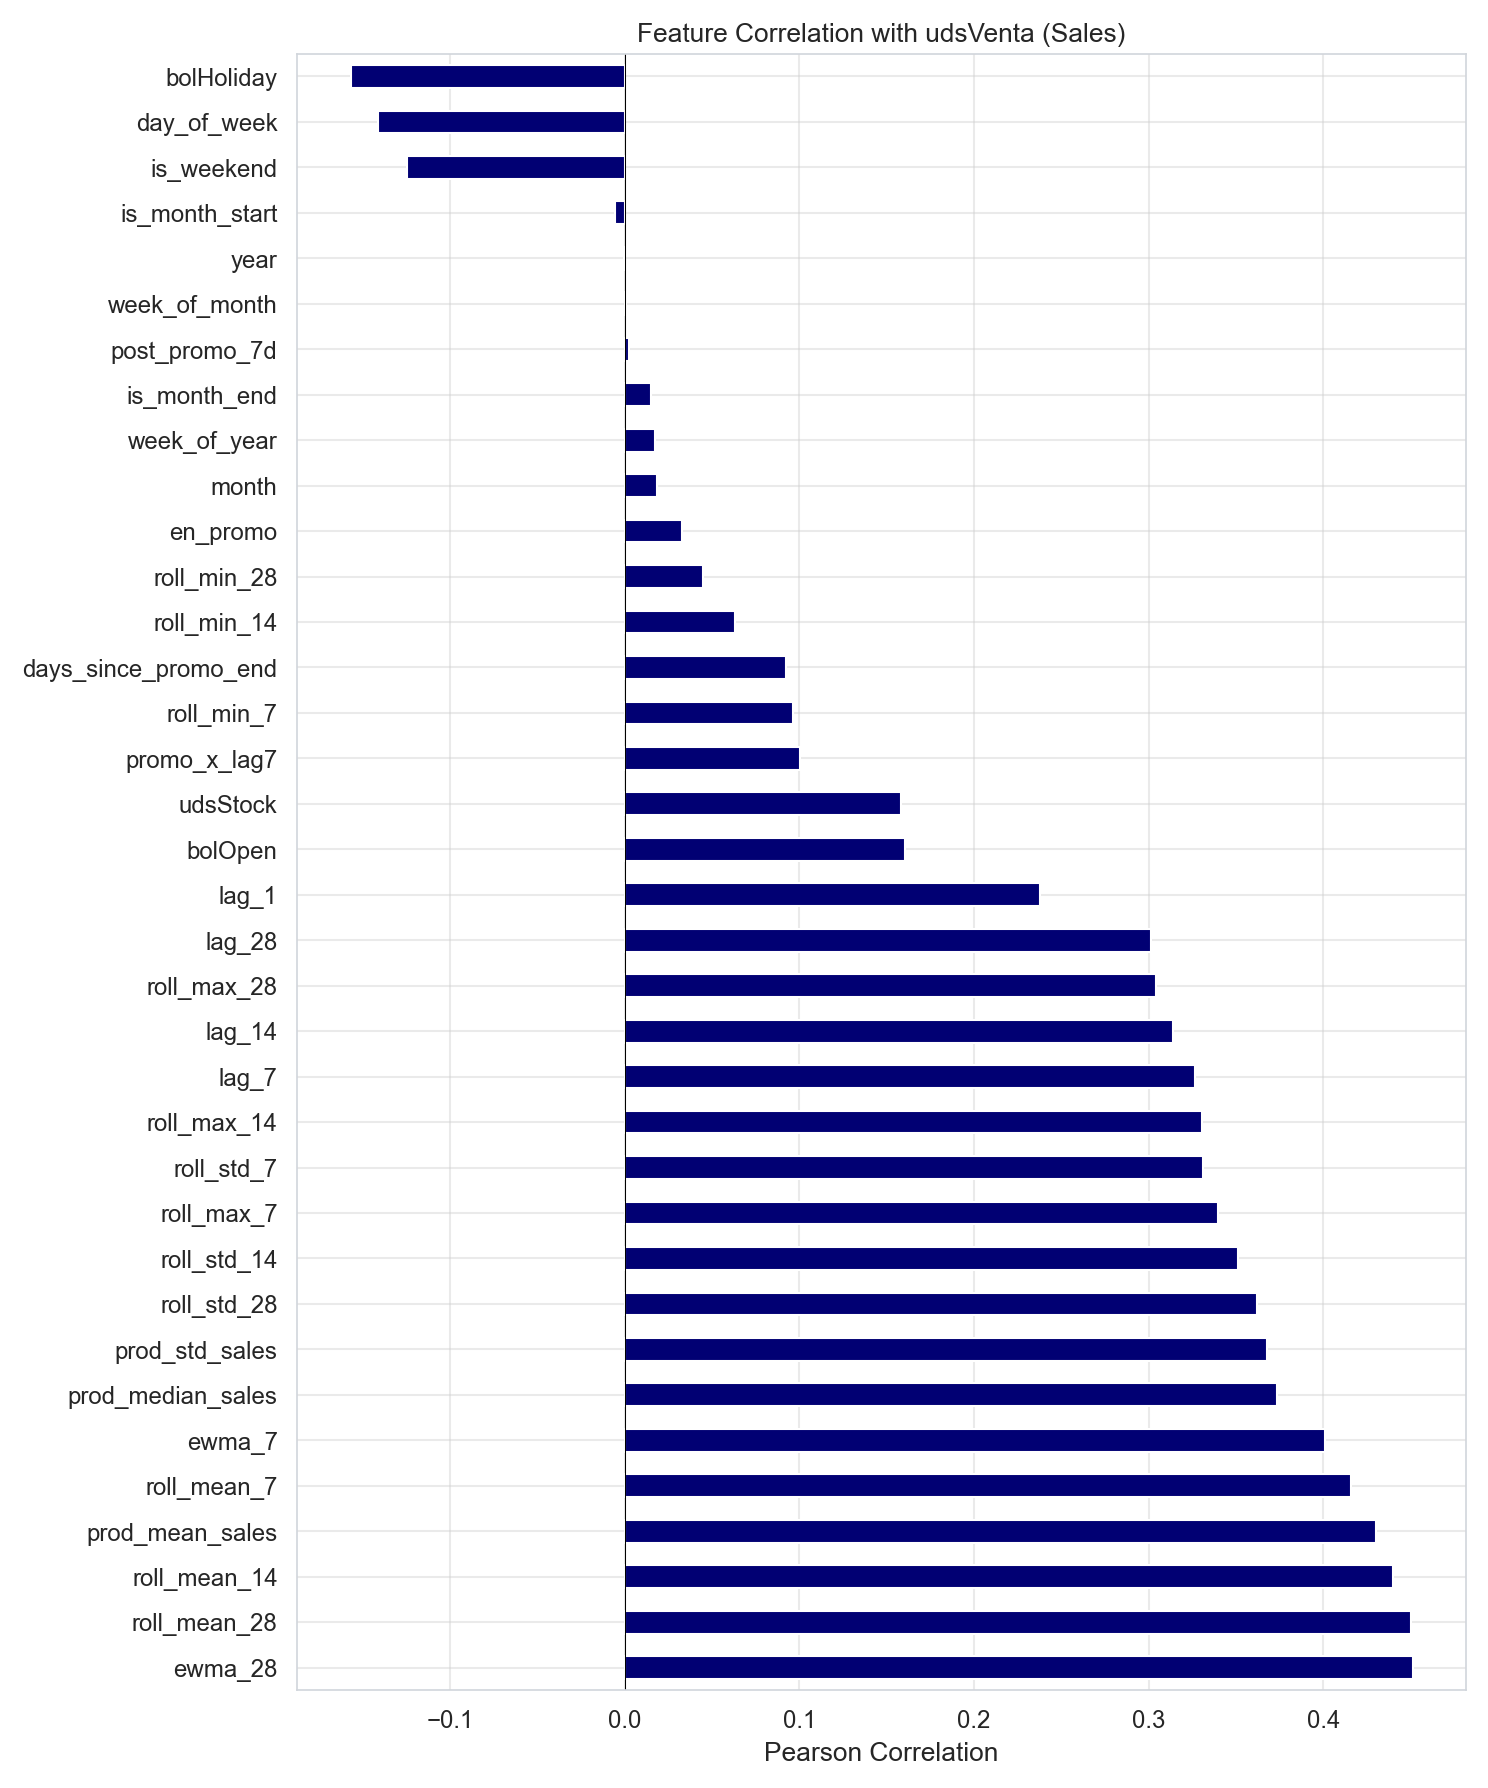
\includegraphics[width=0.95\textwidth]{figures/10_feature_correlations.png}
\caption{Correlation matrix of the engineered features. Strong correlations are visible among rolling statistics at different window sizes, confirming the presence of redundant but complementary temporal signals.}
\label{fig:feature_correlations}
\end{figure}


\section{Modelling}

\subsection{Model Selection}

Four forecasting approaches were implemented, spanning a naive baseline and three gradient boosting / ensemble methods:

\begin{enumerate}
    \item \textbf{Naive baseline (lag-7):} The simplest possible forecast, predicting that demand on any given day equals the demand observed on the same weekday of the previous week. This baseline exploits the strong weekly autocorrelation identified during exploration and provides a meaningful benchmark against which machine learning models must demonstrate improvement.

    \item \textbf{ARIMA (Seasonal):} A classical time series approach fitted per product using the \texttt{auto\_arima} implementation from the \texttt{pmdarima} library. Each product's demand series was modelled with seasonal ARIMA (SARIMA) with weekly periodicity ($m=7$), automatically selecting the optimal $(p,d,q)(P,D,Q)_7$ orders via stepwise search. ARIMA serves as the classical statistical baseline, representing the best that traditional time series methods can achieve without engineered features.

    \item \textbf{Random Forest:} An ensemble of decision trees trained on bootstrap samples with random feature subsets \citep{hyndman2021forecasting}. Random Forest provides robust predictions with built-in protection against overfitting through bagging and feature randomisation.

    \item \textbf{XGBoost:} A gradient boosting framework that builds trees sequentially, with each tree correcting the errors of its predecessors. XGBoost incorporates L1 and L2 regularisation, column subsampling, and efficient handling of sparse data, making it well-suited to the high proportion of zero-demand observations in this dataset.

    \item \textbf{LightGBM:} A gradient boosting implementation that uses histogram-based splitting and leaf-wise tree growth, offering faster training times than XGBoost while maintaining competitive accuracy. LightGBM was among the dominant algorithms in the M5 forecasting competition \citep{makridakis2021m5findings}.

    \item \textbf{LSTM (Long Short-Term Memory):} A recurrent neural network architecture designed to capture long-range temporal dependencies in sequential data \citep{hochreiter1997lstm}. Unlike tree-based methods, which rely on engineered lag features, LSTM processes input data as ordered sequences, with its internal gating mechanism allowing it to selectively retain or discard information from previous time steps. The model was implemented in PyTorch with a single LSTM layer (32 hidden units), trained on standardised features using 14-day input sequences.
\end{enumerate}

All tree-based models were trained on the full set of 33 input features (the 36 engineered features minus the 3 product-level statistics used only for reference). ARIMA was fitted per product on the raw sales series without engineered features, as is standard for classical time series methods. The LSTM model received the same 33 features as the tree models, but processed them as ordered sequences rather than independent observations. All predictions were clipped to a minimum of zero to prevent negative forecast values.

\subsection{Definition of Accuracy Indicators}

Four complementary metrics were used to evaluate forecast performance, as introduced in Chapter~2:

\begin{itemize}
    \item \textbf{MAE} (Mean Absolute Error): average absolute deviation between forecast and actual demand, in the same units as the target variable.
    \item \textbf{RMSE} (Root Mean Squared Error): penalises larger errors more heavily than MAE, providing a measure sensitive to occasional large deviations.
    \item \textbf{MAPE} (Mean Absolute Percentage Error): expresses errors as a percentage of actual demand, computed only for observations where actual demand is greater than zero to avoid division by zero.
    \item \textbf{$\sigma_e$} (forecast error standard deviation): the standard deviation of the residuals ($D_t - F_t$), which directly enters the safety stock calculation (Equation~\ref{eq:safety_stock}) and thus provides the link between forecast accuracy and inventory cost.
\end{itemize}

\subsection{Definition of Training and Validation Periods}

A rolling forecast origin validation strategy was adopted to provide a realistic assessment of out-of-sample performance by simulating the sequential nature of real forecasting decisions \citep{makridakis2021m5findings}.

Three validation folds were defined, each with a 30-day test window, working backwards from the most recent date in the dataset:

\begin{table}[H]
\centering
\small
\caption{Rolling forecast origin validation folds.}
\label{tab:folds}
\begin{tabular}{|c|c|c|c|}
\hline
\textbf{Fold} & \textbf{Training period end} & \textbf{Test period} & \textbf{Test days} \\
\hline
1 & 2024-09-06 & 2024-09-07 -- 2024-10-06 & 30 \\
2 & 2024-10-06 & 2024-10-07 -- 2024-11-05 & 30 \\
3 & 2024-10-06 & 2024-10-07 -- 2024-11-05 & 30 \\
\hline
\end{tabular}
\end{table}

For each fold, the training set includes all data up to the fold's cutoff date (expanding window), and the model is evaluated on the subsequent 30-day period. Final reported metrics are averaged across all three folds.

\subsection{Hyperparameter Tuning}

Hyperparameters for all three machine learning models were optimised using Optuna \citep{makridakis2021m5findings}, a Bayesian optimisation framework that efficiently explores the parameter space using a Tree-structured Parzen Estimator (TPE) sampler.

To balance computational cost with tuning quality, the optimisation was conducted on a representative subset of 50 randomly sampled products using the first validation fold. Each model was allocated 30 Optuna trials, with RMSE on the validation set as the objective function. The optimised hyperparameters were then applied to the full dataset across all validation folds.

Table~\ref{tab:tuned_params} presents the key tuned hyperparameters for each model:

\begin{table}[H]
\centering
\small
\caption{Optimised hyperparameters via Optuna (30 trials per model).}
\label{tab:tuned_params}
\begin{tabular}{|l|l|r|}
\hline
\textbf{Model} & \textbf{Parameter} & \textbf{Value} \\
\hline
\multirow{5}{*}{LightGBM} & n\_estimators & 300 \\
 & learning\_rate & 0.011 \\
 & num\_leaves & 75 \\
 & max\_depth & 4 \\
 & min\_child\_samples & 25 \\
\hline
\multirow{5}{*}{XGBoost} & n\_estimators & 350 \\
 & learning\_rate & 0.019 \\
 & max\_depth & 3 \\
 & min\_child\_weight & 10 \\
 & subsample & 0.90 \\
\hline
\multirow{4}{*}{Random Forest} & n\_estimators & 100 \\
 & max\_depth & 5 \\
 & min\_samples\_leaf & 16 \\
 & max\_features & 0.30 \\
\hline
\end{tabular}
\end{table}

The relatively shallow tree depths (3--5) and conservative learning rates (0.011--0.019) selected by the optimiser suggest that the models benefit from regularisation, which is consistent with the high proportion of zero-demand observations in the dataset.


\section{Evaluation}

\subsection{Accuracy Results Obtained}

Table~\ref{tab:results_summary} presents the average performance of each model across the three validation folds:

\begin{table}[H]
\centering
\small
\caption{Average forecast accuracy across three rolling validation folds.}
\label{tab:results_summary}
\begin{tabular}{|l|r|r|r|r|}
\hline
\textbf{Model} & \textbf{MAE} & \textbf{RMSE} & \textbf{MAPE (\%)} & \textbf{$\sigma_e$} \\
\hline
XGBoost & 1.366 & 2.155 & 52.2 & 2.154 \\
LightGBM & 1.373 & 2.158 & 51.7 & 2.158 \\
Random Forest & 1.394 & 2.176 & 51.6 & 2.176 \\
ARIMA$^\dagger$ & 1.443 & 2.220 & 59.8 & 2.219 \\
LSTM & 1.522 & 2.235 & 49.8 & 2.223 \\
Naive (lag-7) & 1.661 & 3.091 & 86.0 & 3.091 \\
\hline
\end{tabular}
\begin{flushleft}
\footnotesize{$^\dagger$ ARIMA evaluated on 50 sampled products due to per-product fitting cost.}
\end{flushleft}
\end{table}

All three tree-based machine learning models substantially outperform both the naive baseline and the classical/deep learning alternatives. XGBoost achieves the lowest RMSE (2.155), followed closely by LightGBM (2.158) and Random Forest (2.176). The RMSE improvement over the naive baseline ranges from 27.9\% (LSTM) to 30.3\% (XGBoost).

\begin{figure}[H]
\centering
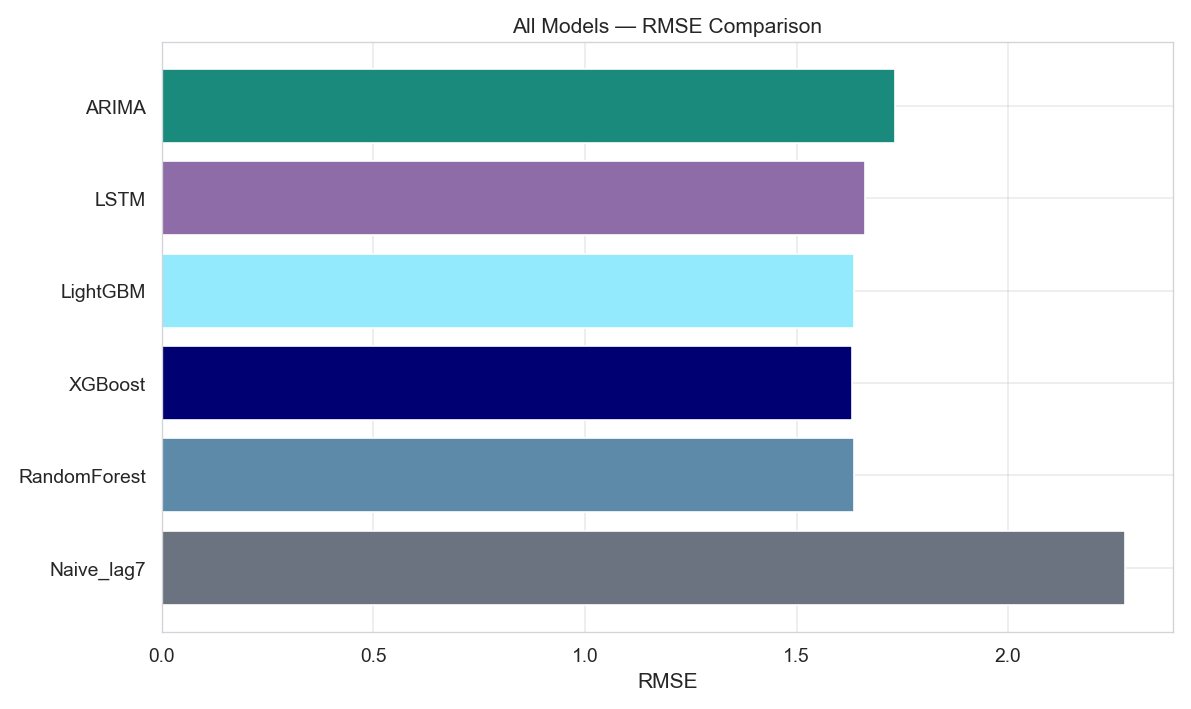
\includegraphics[width=0.85\textwidth]{figures/24_all_models_comparison.png}
\caption{Comparison of forecast accuracy (RMSE) across all six models. The three tree-based models form a tight cluster, substantially outperforming both classical and deep learning alternatives.}
\label{fig:all_models_comparison}
\end{figure}

ARIMA and LSTM occupy an intermediate position: both significantly outperform the naive baseline (RMSE reductions of 28.2\% and 27.7\% respectively) but fall short of the tree-based models. This result is consistent with the findings of the M5 forecasting competition \citep{makridakis2021m5findings}, where gradient boosting algorithms consistently outperformed both classical statistical methods and standalone deep learning approaches. The LSTM's slightly lower MAPE (49.8\%) but higher RMSE suggests it handles the zero-heavy distribution differently from tree models, producing fewer large percentage errors but occasionally larger absolute deviations.

\subsection{Comparison of Results Across Models}

\textbf{Promotional vs. non-promotional performance.} Table~\ref{tab:promo_results} compares model performance across demand segments:

\begin{table}[H]
\centering
\small
\caption{Model performance by demand segment (last validation fold).}
\label{tab:promo_results}
\begin{tabular}{|l|l|r|r|r|r|}
\hline
\textbf{Segment} & \textbf{Model} & \textbf{MAE} & \textbf{RMSE} & \textbf{MAPE (\%)} & \textbf{$\sigma_e$} \\
\hline
\multirow{4}{*}{Non-Promo} & XGBoost & 1.299 & 2.055 & 52.3 & 2.055 \\
 & LightGBM & 1.308 & 2.058 & 51.8 & 2.058 \\
 & Random Forest & 1.327 & 2.073 & 51.6 & 2.073 \\
 & Naive (lag-7) & 1.565 & 2.969 & 85.9 & 2.969 \\
\hline
\multirow{4}{*}{Promo} & XGBoost & 1.917 & 2.844 & 51.7 & 2.836 \\
 & LightGBM & 1.911 & 2.851 & 51.4 & 2.838 \\
 & Random Forest & 1.944 & 2.884 & 51.6 & 2.873 \\
 & Naive (lag-7) & 2.448 & 3.956 & 86.9 & 3.955 \\
\hline
\end{tabular}
\end{table}

Promotional demand is consistently harder to predict across all models, with RMSE values approximately 38\% higher than for non-promotional periods. However, the ML models maintain their advantage over the naive baseline in both segments, with RMSE improvements of approximately 28\% for non-promotional and 28\% for promotional demand.

\textbf{Per-product RMSE distribution.} Analysis at the individual product level reveals that LightGBM achieves a median per-product RMSE of 1.65, compared to 2.36 for the naive baseline. The improvement is not uniform: some products see RMSE reductions exceeding 15 units, while approximately 10 products show marginally worse performance with ML than with the naive approach. These products tend to have very low and stable demand where the simple lag-7 heuristic is already near-optimal.

\begin{figure}[H]
\centering
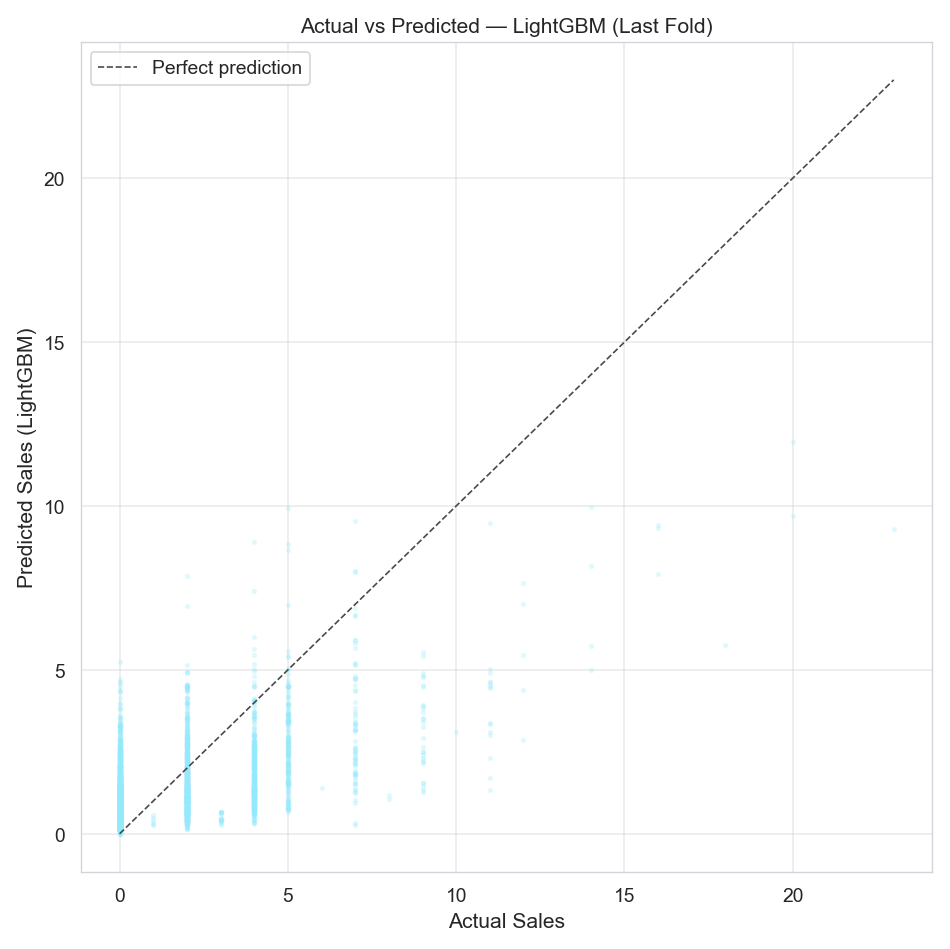
\includegraphics[width=0.85\textwidth]{figures/13_actual_vs_predicted_lgbm.png}
\caption{Actual vs.\ predicted sales for LightGBM on a sample of products. Points near the diagonal indicate accurate predictions; the cluster near the origin reflects the high proportion of zero-demand observations.}
\label{fig:actual_vs_predicted}
\end{figure}

\begin{figure}[H]
\centering
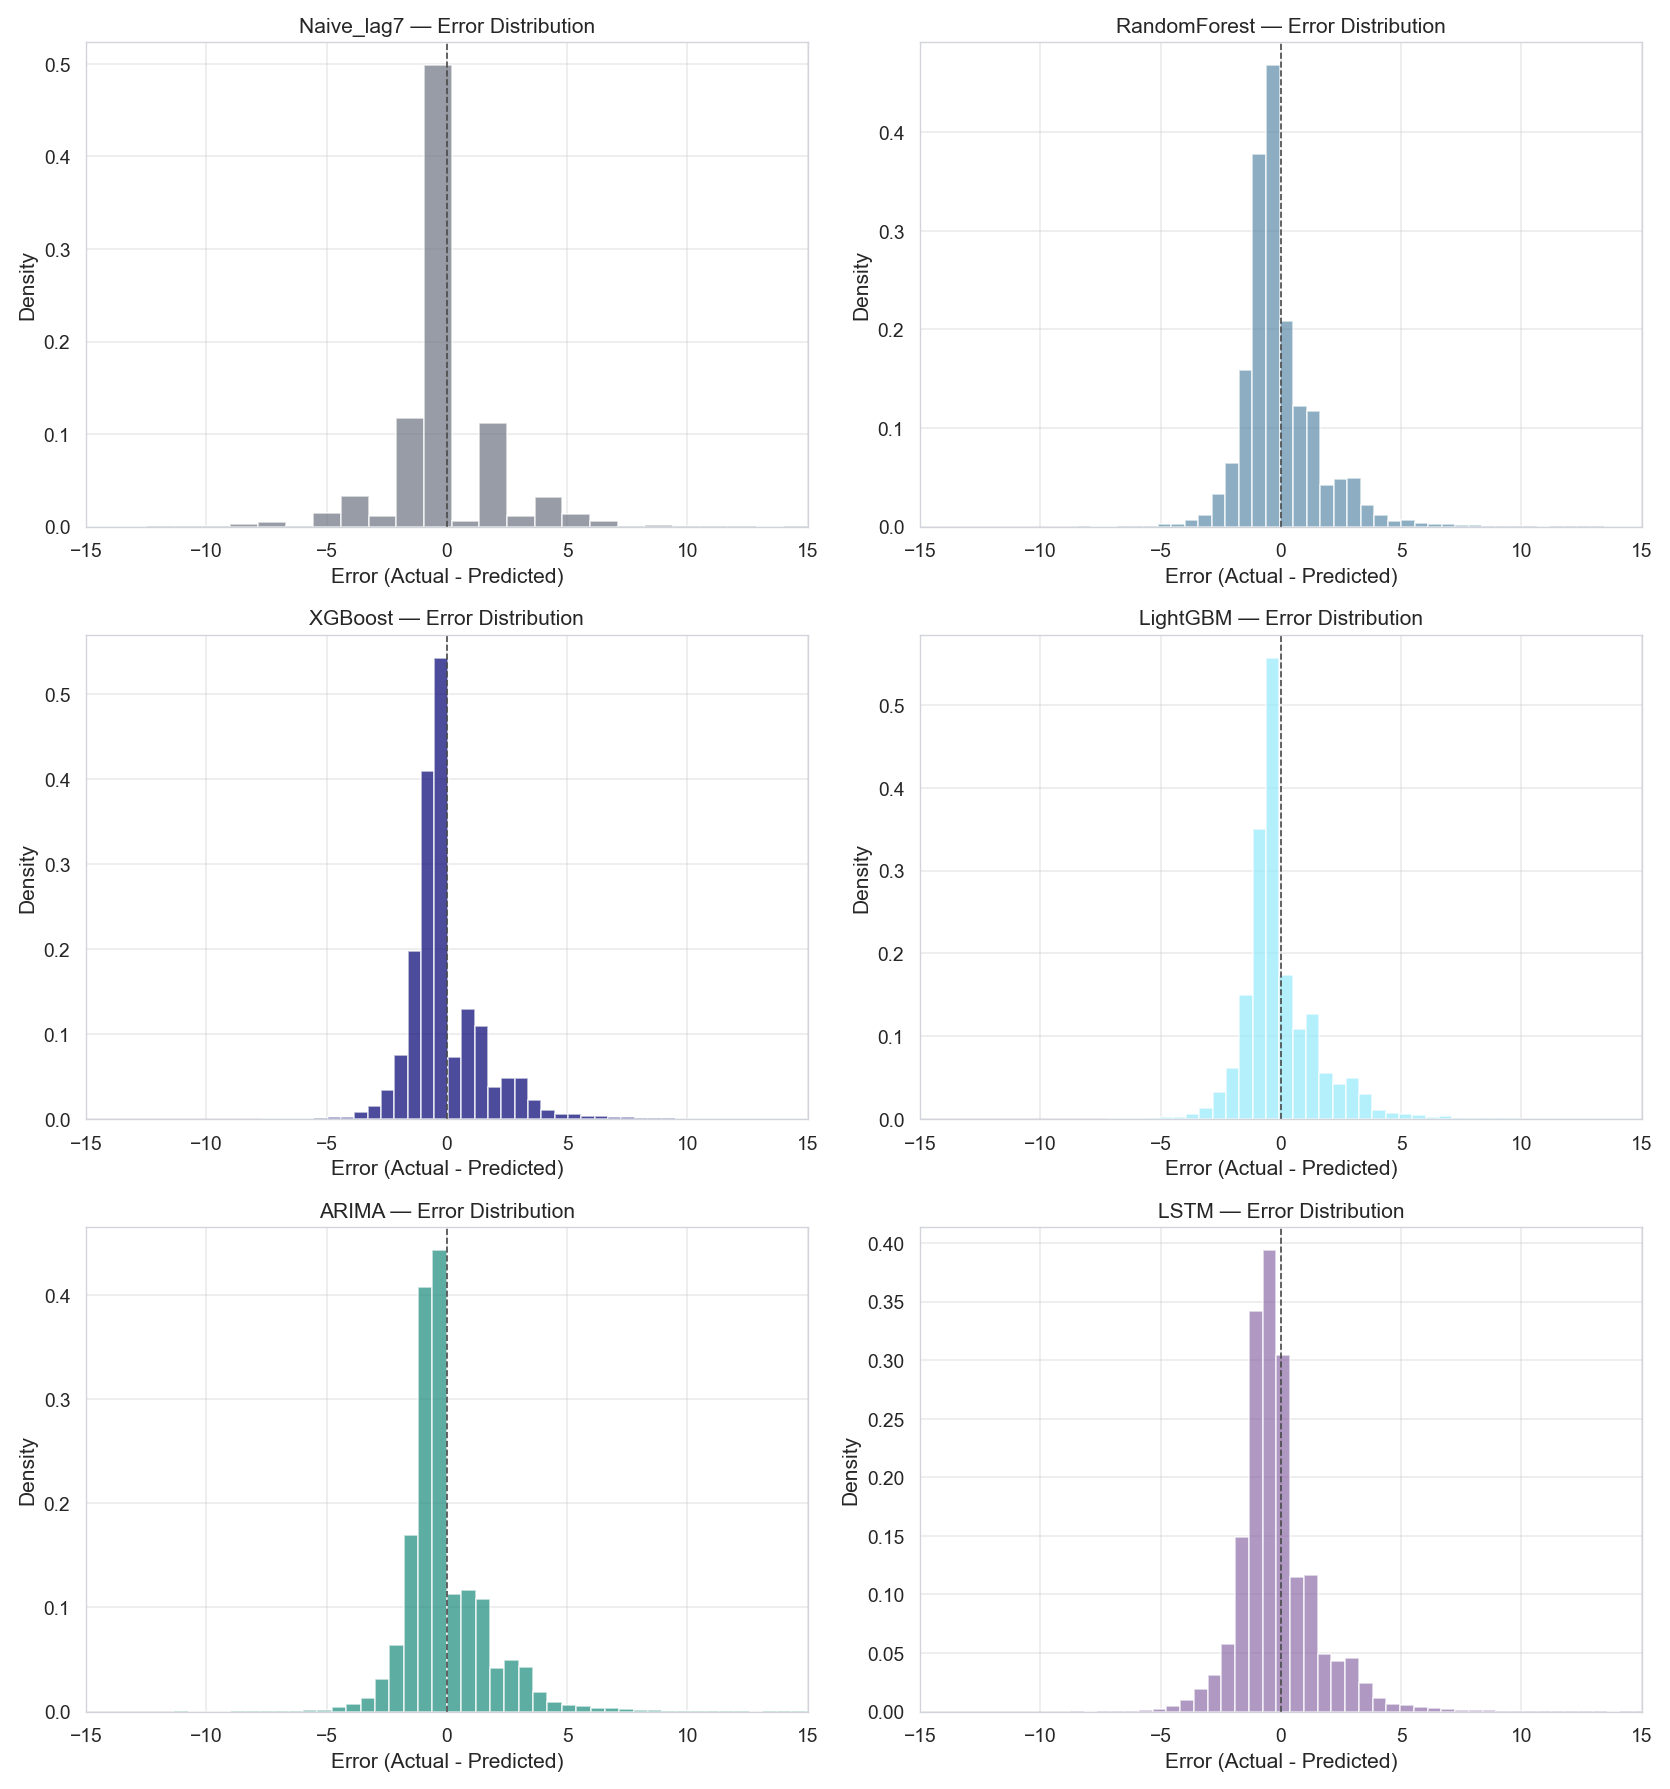
\includegraphics[width=0.85\textwidth]{figures/17_error_distributions.png}
\caption{Distribution of forecast errors by model. The ML models produce tighter, more symmetric error distributions compared to the naive baseline.}
\label{fig:error_distributions}
\end{figure}

\begin{figure}[H]
\centering
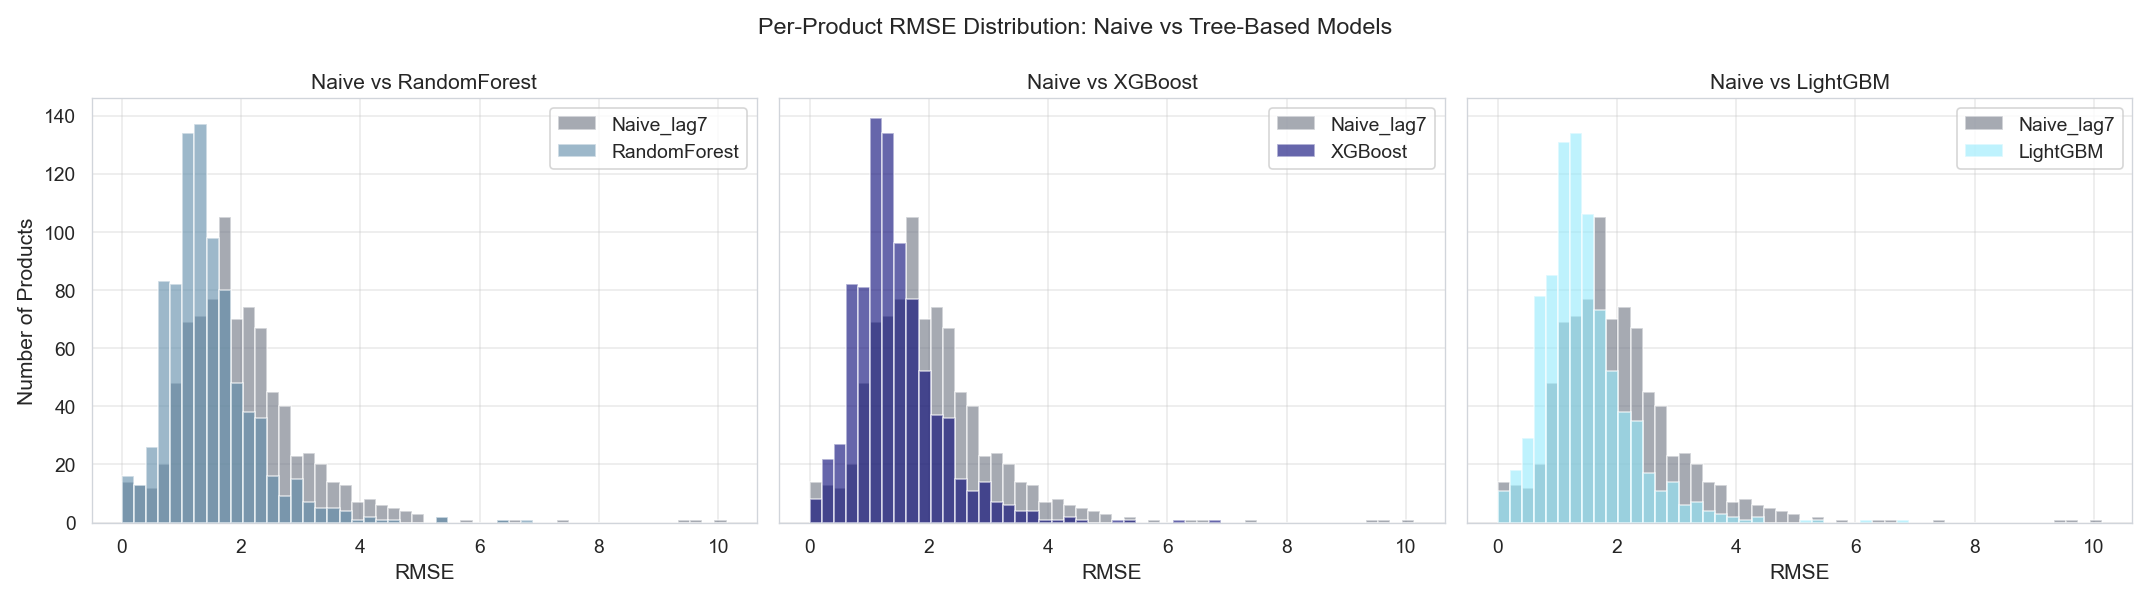
\includegraphics[width=0.85\textwidth]{figures/18_per_product_rmse_dist.png}
\caption{Distribution of per-product RMSE values. The ML models shift the distribution towards lower RMSE values compared to the naive baseline.}
\label{fig:per_product_rmse}
\end{figure}

\textbf{SHAP feature importance.} To understand the drivers of model predictions, SHAP (SHapley Additive exPlanations) analysis was performed on the LightGBM model. Table~\ref{tab:shap_top10} presents the ten most influential features:

\begin{table}[H]
\centering
\small
\caption{Top 10 features by mean absolute SHAP value (LightGBM).}
\label{tab:shap_top10}
\begin{tabular}{|r|l|r|}
\hline
\textbf{Rank} & \textbf{Feature} & \textbf{Mean $|$SHAP$|$} \\
\hline
1 & ewma\_28 & 0.524 \\
2 & bolHoliday & 0.295 \\
3 & roll\_mean\_28 & 0.150 \\
4 & day\_of\_week & 0.079 \\
5 & udsStock & 0.063 \\
6 & roll\_max\_28 & 0.046 \\
7 & lag\_28 & 0.025 \\
8 & bolOpen & 0.022 \\
9 & roll\_mean\_14 & 0.017 \\
10 & roll\_max\_14 & 0.016 \\
\hline
\end{tabular}
\end{table}

The 28-day EWMA emerges as the single most important predictor, followed by the holiday indicator and the 28-day rolling mean. This confirms that the model relies heavily on smoothed representations of recent demand history, with calendar effects providing secondary but significant predictive power. Notably, the longer-horizon features (28-day windows) dominate over shorter-horizon ones (7-day), suggesting that the model captures medium-term demand trends rather than relying solely on short-term momentum.

\begin{figure}[H]
\centering
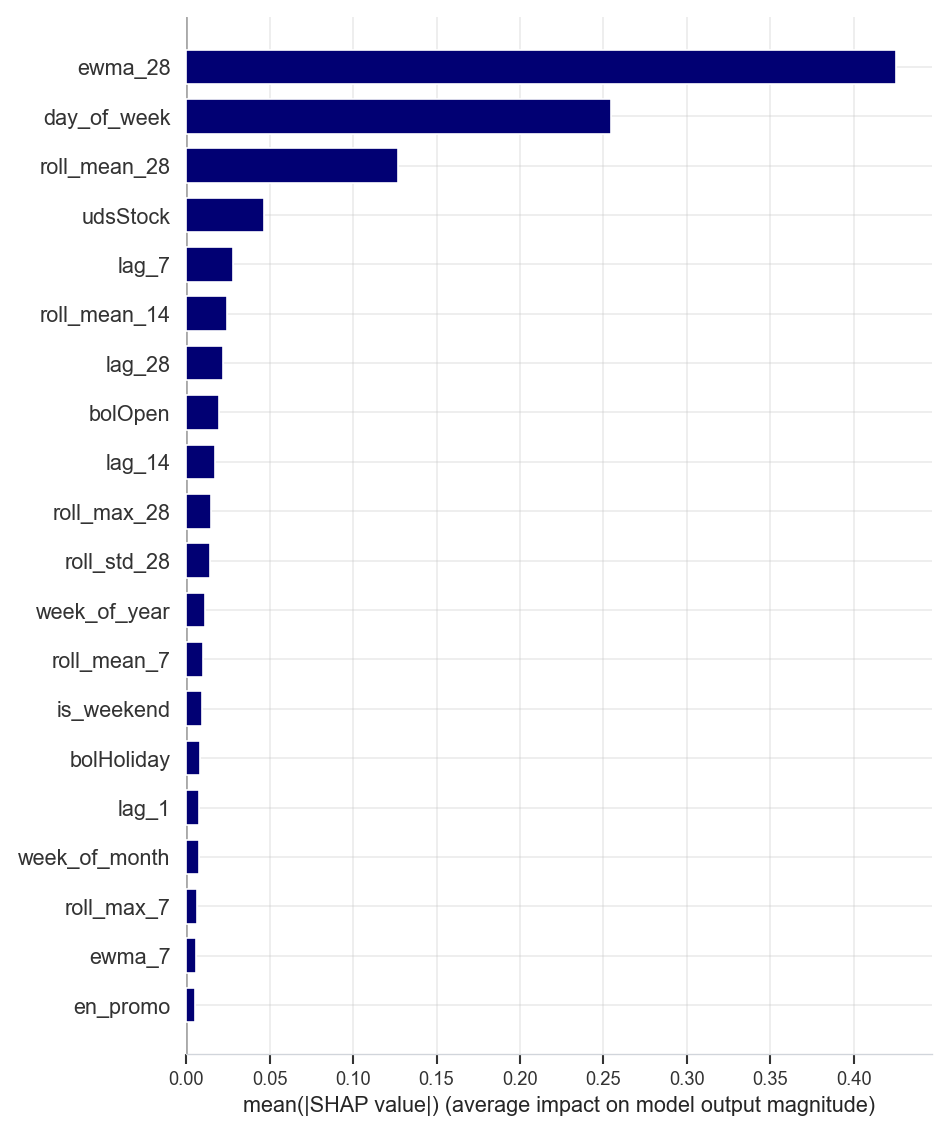
\includegraphics[width=0.85\textwidth]{figures/15_shap_bar.png}
\caption{SHAP feature importance (mean absolute SHAP values) for LightGBM. The 28-day EWMA dominates, followed by calendar and rolling statistics features.}
\label{fig:shap_bar}
\end{figure}

\begin{figure}[H]
\centering
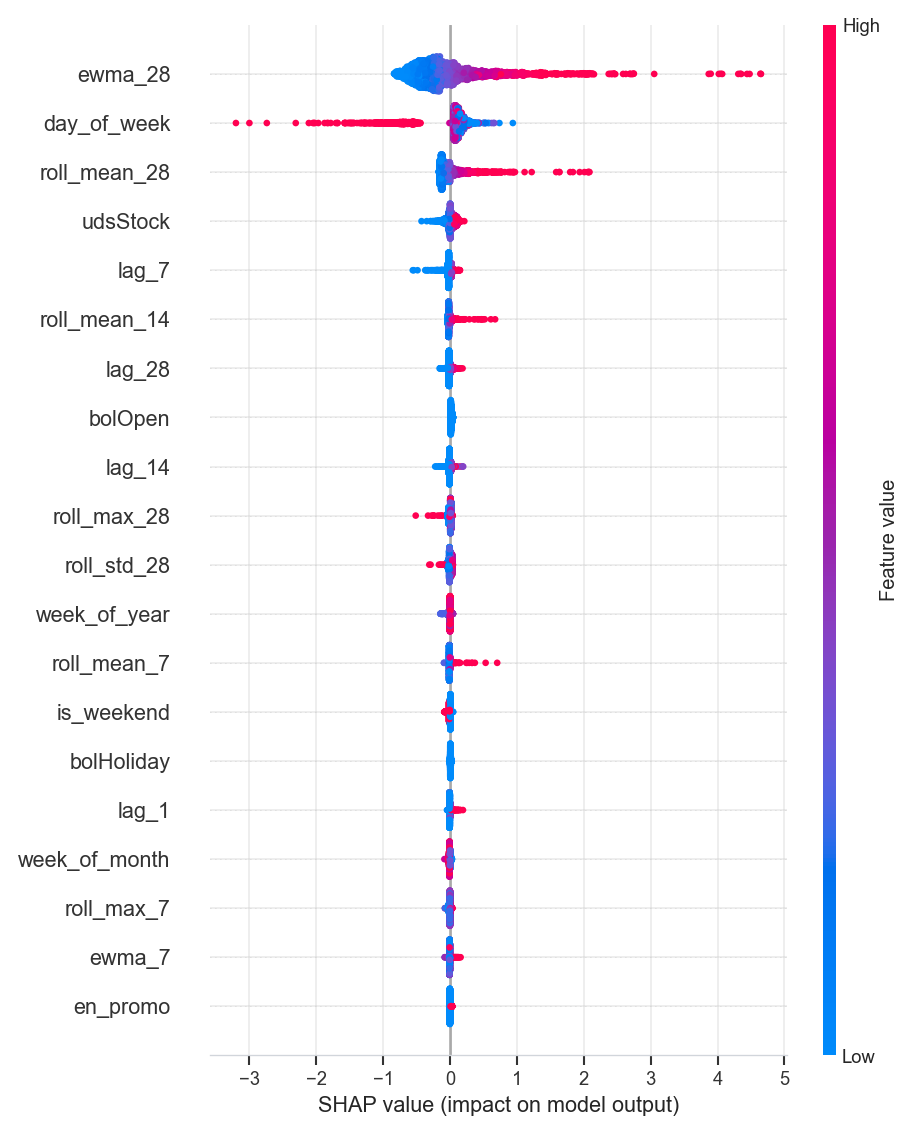
\includegraphics[width=0.85\textwidth]{figures/14_shap_summary.png}
\caption{SHAP summary plot showing the direction and magnitude of feature effects. Red indicates high feature values; blue indicates low values. High \texttt{ewma\_28} values push predictions upward, consistent with higher recent demand leading to higher forecasts.}
\label{fig:shap_summary}
\end{figure}

\subsection{Conclusions from Results}

The evaluation yields several key findings:

\begin{enumerate}
    \item The three tree-based machine learning models (XGBoost, LightGBM, Random Forest) achieve the best performance, with RMSE values within 1\% of each other. This suggests that the feature engineering, rather than the specific algorithm choice, is the primary driver of forecast quality among this model family.

    \item ARIMA and LSTM occupy an intermediate tier, both significantly outperforming the naive baseline (RMSE reductions of 28\% and 28\% respectively) but falling short of the tree-based models. ARIMA's per-product fitting captures local demand patterns effectively but cannot leverage cross-product information or engineered features. LSTM captures sequential dependencies but requires substantially more training data and computation to match tree-based performance.

    \item The improvement over the naive baseline is substantial across all ML approaches (28--30\% RMSE reduction), demonstrating the value of incorporating engineered features and systematic model training over simple heuristic forecasting.

    \item Promotional demand remains the most challenging segment, with RMSE approximately 38\% higher than non-promotional demand across all models. However, the ML models maintain their relative advantage over the baseline in both segments.

    \item SHAP analysis reveals that smoothed demand history (EWMA and rolling statistics) and calendar features are the most influential predictors, validating the feature engineering strategy adopted in this work.

    \item The forecast error standard deviation ($\sigma_e \approx 2.15$ for the best tree models, $\sigma_e \approx 2.22$ for ARIMA/LSTM, compared to $\sigma_e \approx 3.09$ for the naive baseline) translates directly into safety stock reductions, as quantified in the following section.
\end{enumerate}


\section{Impact of Algorithm Improvement}

\subsection{Impact on Processes}

The transition from a naive forecasting approach to machine learning models has implications beyond numerical accuracy improvements. From an operational perspective, the key process impacts are:

\textbf{Safety stock reduction.} Using the safety stock formulation from Equation~\ref{eq:safety_stock} with a 95\% service level ($z = 1.645$) and a protection period of 10 days (3 days lead time + 7 days review period), the total safety stock across all 894 products decreases from 11,953 units under the naive forecast to 8,276 units under LightGBM --- a reduction of 30.8\%. This means that the same service level can be maintained with significantly less inventory investment.

\textbf{Forecast error symmetry.} Analysis of error distributions shows that the ML models produce approximately symmetric errors centred near zero, whereas the naive baseline exhibits a slight positive bias (tendency to overforecast). Symmetric errors are preferable for inventory planning, as they indicate that the forecast is equally likely to overestimate or underestimate demand, allowing safety stock to function as intended.

\textbf{Sensitivity to service level.} Table~\ref{tab:sensitivity} presents the total safety stock requirements across different service levels:

\begin{table}[H]
\centering
\small
\caption{Total safety stock (units) by model and service level.}
\label{tab:sensitivity}
\begin{tabular}{|l|r|r|r|}
\hline
\textbf{Model} & \textbf{90\%} & \textbf{95\%} & \textbf{99\%} \\
\hline
LightGBM & 6,450 & 8,276 & 11,702 \\
XGBoost & 6,466 & 8,296 & 11,731 \\
Random Forest & 6,507 & 8,350 & 11,806 \\
Naive (lag-7) & 9,316 & 11,953 & 16,902 \\
\hline
\end{tabular}
\end{table}

The ML models consistently require approximately 30\% less safety stock than the naive baseline across all service levels, demonstrating that the improvement is robust and not dependent on a specific service level assumption.

\begin{figure}[H]
\centering
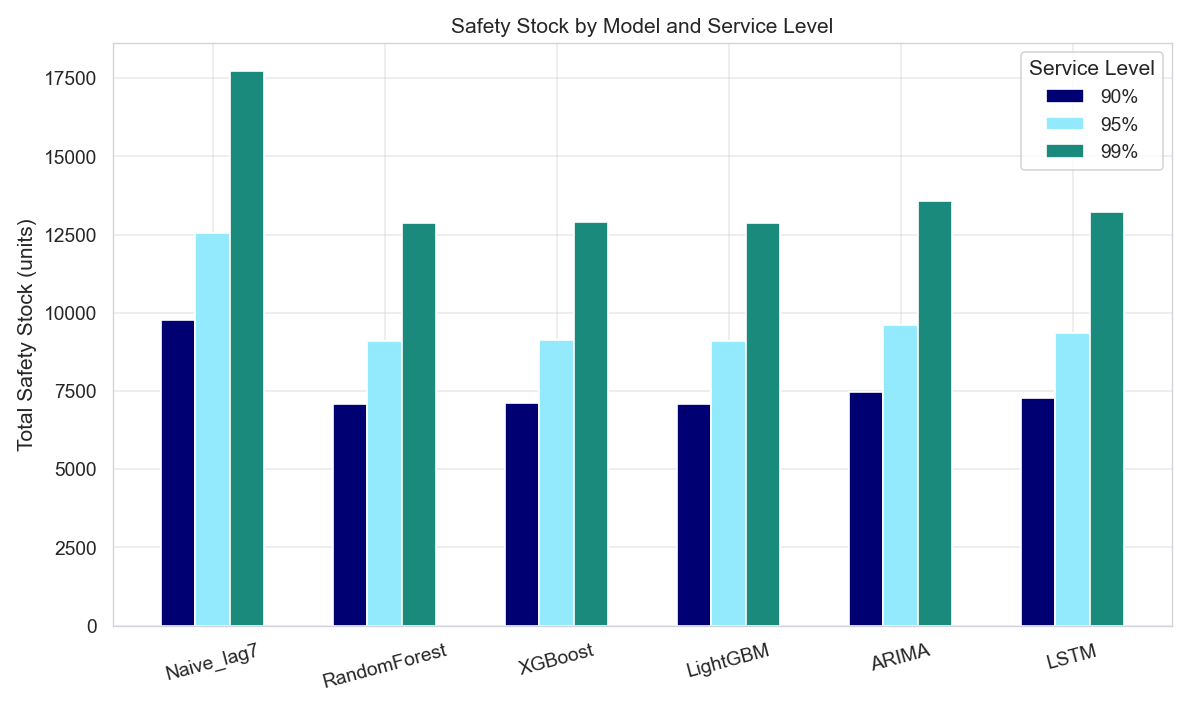
\includegraphics[width=0.85\textwidth]{figures/21_safety_stock_by_service_level.png}
\caption{Total safety stock requirements by model and service level. The ML models maintain a consistent ~30\% advantage over the naive baseline across all service levels.}
\label{fig:safety_stock_service_level}
\end{figure}

\subsection{Economic Impact}

The economic impact analysis combines two cost components: the newsvendor cost (direct cost of forecast errors) and the safety stock holding cost.

\textbf{Newsvendor cost analysis.} Following the total cost formulation from Equation~\ref{eq:total_cost}, the asymmetric costs of overforecasting and underforecasting were computed using cost parameters of $C_o = \text{\euro}0.10$ per unit per day (overage/holding) and $C_u = \text{\euro}0.50$ per unit per day (underage/lost sale), yielding a critical ratio of 0.83. These values reflect a typical retail/industrial setting where stockout costs substantially exceed holding costs.

Table~\ref{tab:newsvendor} presents the newsvendor cost results:

\begin{table}[H]
\centering
\small
\caption{Newsvendor cost analysis (30-day test period, annualised).}
\label{tab:newsvendor}
\begin{tabular}{|l|r|r|r|r|}
\hline
\textbf{Model} & \textbf{Overage (€)} & \textbf{Underage (€)} & \textbf{Total (€)} & \textbf{Annual est. (€)} \\
\hline
Naive (lag-7) & 2,227 & 11,138 & 13,365 & 162,603 \\
Random Forest & 1,830 & 9,538 & 11,367 & 138,304 \\
LightGBM & 1,786 & 9,489 & 11,275 & 137,182 \\
XGBoost & 1,785 & 9,392 & 11,176 & 135,979 \\
\hline
\end{tabular}
\end{table}

XGBoost achieves the lowest newsvendor cost, saving approximately \euro26,600 annually (16.4\%) compared to the naive baseline. Underage costs dominate in all models, consistent with the asymmetric cost structure where stockouts are five times more expensive than excess inventory.

\textbf{Combined cost analysis.} Table~\ref{tab:combined_cost} presents the total annual cost combining newsvendor costs with safety stock holding costs at the 95\% service level:

\begin{table}[H]
\centering
\small
\caption{Combined annual cost: newsvendor + safety stock holding (95\% service level).}
\label{tab:combined_cost}
\begin{tabular}{|l|r|r|r|}
\hline
\textbf{Model} & \textbf{Newsvendor (€/yr)} & \textbf{SS Holding (€/yr)} & \textbf{Total (€/yr)} \\
\hline
Naive (lag-7) & 162,603 & 436,294 & 598,896 \\
Random Forest & 138,304 & 304,763 & 443,067 \\
LightGBM & 137,182 & 302,083 & 439,265 \\
XGBoost & 135,979 & 302,816 & 438,796 \\
\hline
\end{tabular}
\end{table}

The ML models achieve total annual cost savings of approximately \euro160,000 (26.7\%) compared to the naive baseline. XGBoost and LightGBM perform nearly identically in economic terms, with XGBoost holding a marginal advantage of \euro469 annually.

\begin{figure}[H]
\centering
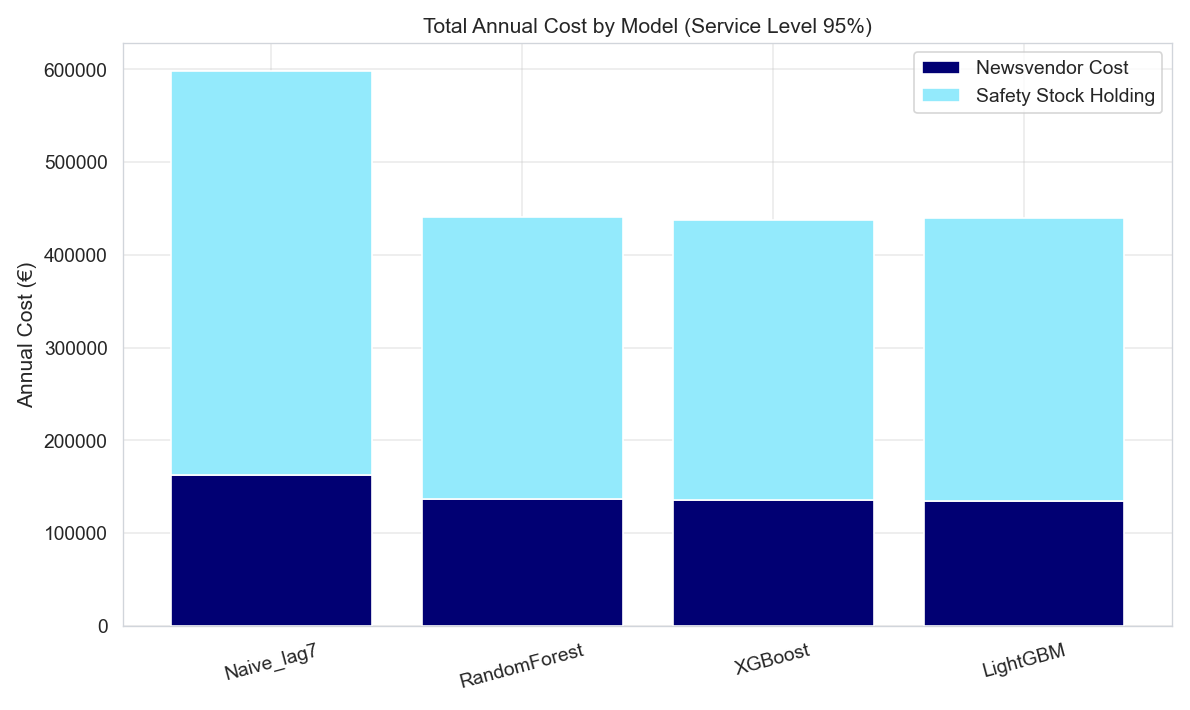
\includegraphics[width=0.85\textwidth]{figures/22_combined_annual_cost.png}
\caption{Combined annual inventory cost (newsvendor + safety stock holding) by model. The ML models reduce total costs by approximately 26.7\% compared to the naive baseline.}
\label{fig:combined_annual_cost}
\end{figure}

These results demonstrate that the forecast accuracy improvements documented in Section~3.6 translate into meaningful economic benefits. The 28\% reduction in RMSE corresponds to a 26.7\% reduction in total inventory-related costs, confirming the theoretical relationship between forecast error and inventory costs established in Chapter~2 (Equations~\ref{eq:ss_cost} and \ref{eq:total_cost}).

It is important to note that the cost parameters used in this analysis ($C_o$ and $C_u$) are illustrative values chosen to reflect typical industrial cost structures. The relative ranking of models and the percentage savings are robust to reasonable variations in these parameters, as the underlying driver is the reduction in forecast error rather than the specific cost assumptions. A sensitivity analysis across service levels (Table~\ref{tab:sensitivity}) confirms that the ML advantage is maintained regardless of the risk tolerance adopted by the organisation.
